\documentclass[fleqn,8pt,t]{beamer}

\usepackage[french]{babel}
\usepackage[utf8]{inputenc}
\usepackage[T1]{fontenc}
%\usepackage{french} % Sommaire en début de document
%\usepackage[top=2cm, bottom=2cm, left=2cm, right=2cm]{geometry} % Marges

\usepackage{amsmath} % Maths
\usepackage{amsfonts} % Maths
\usepackage{amssymb} % Maths
\usepackage{stmaryrd} % Maths (crochets doubles)

%\usepackage{listings} % Mise en forme du code (pour Hoare) ## À REVOIR ###
%\usepackage{ifthen} % Structures If Then Else
\usepackage{theorem} % Styles supplémentaires pour théorèmes
\usepackage{url}
\usepackage{xcolor,colortbl} % Cellules colorées
\usepackage{array}  % Tableaux évolués
\usepackage{multirow}  % Pour des colonnes sur plusieurs lignes

%\usepackage{enumerate} % Changer les puces des listes d'énumération
%\usepackage{setspace} % Changer les interlignes

%\usepackage{subfig} % Créer des sous-figures
%\usepackage{graphicx} % Importer des images
\usepackage{tikz}

\usepackage{ulem}  % Pour l'attribut barré

\usepackage{comment}

% Police
\usepackage{lmodern}
%\usepackage{libertine}
% \usepackage{ziffer}     % Typographie française pour les nombres
% \ZifferAus
%\ZifferAn


% Macros relatives à la traduction de PH avec arcs neutralisants vers PH à k-priorités fixes

% Macros générales
%\newcommand{\ie}{\textit{i.e.} }
\newcommand{\segm}[2]{\llbracket #1; #2 \rrbracket}
%\newcommand{\f}[1]{\mathsf{#1}}

% Notations générales pour PH
\newcommand{\PH}{\mathcal{PH}}
%\newcommand{\PHs}{\mathcal{S}}
\newcommand{\PHs}{\Sigma}
%\newcommand{\PHp}{\mathcal{P}}
\newcommand{\PHp}{\textcolor{red}{\mathcal{P}}}
%\newcommand{\PHproc}{\mathcal{P}}
\newcommand{\PHproc}{\mathbf{Proc}}
\newcommand{\Proc}{\PHproc}
\newcommand{\PHh}{\mathcal{H}}
\newcommand{\PHa}{\PHh}
%\newcommand{\PHa}{\mathcal{A}}
\newcommand{\PHl}{\mathcal{L}}

\newcommand{\PHhitter}{\mathsf{hitter}}
\newcommand{\PHtarget}{\mathsf{target}}
\newcommand{\PHbounce}{\mathsf{bounce}}
%\newcommand{\PHsort}{\Sigma}
\newcommand{\PHsort}{\PHs}

%\newcommand{\PHfrappeur}{\mathsf{frappeur}}
%\newcommand{\PHcible}{\mathsf{cible}}
%\newcommand{\PHbond}{\mathsf{bond}}
%\newcommand{\PHsorte}{\mathsf{sorte}}
%\newcommand{\PHbloquant}{\mathsf{bloquante}}
%\newcommand{\PHbloque}{\mathsf{bloquee}}

%\newcommand{\PHfrappeR}{\textcolor{red}{\rightarrow}}
%\newcommand{\PHmonte}{\textcolor{red}{\Rsh}}

\newcommand{\PHhitA}{\rightarrow}
\newcommand{\PHhitB}{\Rsh}
%\newcommand{\PHfrappe}[3]{\mbox{$#1\PHhitA#2\PHhitB#3$}}
%\newcommand{\PHfrappebond}[2]{\mbox{$#1\PHhitB#2$}}
\newcommand{\PHhit}[3]{#1\PHhitA#2\PHhitB#3}
\newcommand{\PHfrappe}{\PHhit}
\newcommand{\PHhbounce}[2]{#1\PHhitB#2}
\newcommand{\PHobj}[2]{\mbox{$#1\PHhitB^*\!#2$}}
\newcommand{\PHobjectif}{\PHobj}
\newcommand{\PHconcat}{::}
%\newcommand{\PHneutralise}{\rtimes}

\def\PHget#1#2{{#1[#2]}}
%\newcommand{\PHchange}[2]{#1\langle #2 \rangle}
%\newcommand{\PHchange}[2]{(#1 \Lleftarrow #2)}
%\newcommand{\PHarcn}[2]{\mbox{$#1\PHneutralise#2$}}
\newcommand{\PHplay}{\cdot}

\newcommand{\PHstate}[1]{\mbox{$\langle #1 \rangle$}}
\newcommand{\PHetat}{\PHstate}

\def\supp{\mathsf{support}}
\def\first{\mathsf{first}}
\def\last{\mathsf{last}}

\def\DNtrans{\rightarrow_{ADN}}
\def\DNdef{(\mathbb F, \langle f^1, \dots, f^n\rangle)}
\def\DNdep{\mathsf{dep}}
\def\PHPtrans{\rightarrow_{PH}}
\def\get#1#2{#1[{#2}]}
\def\encodeF#1{\mathbf{#1}}
\def\toPH{\encodeF{PH}}
\def\card#1{|#1|}
\def\decode#1{\llbracket#1\rrbracket}
\def\encode#1{\llparenthesis#1\rrparenthesis}
\def\Hits{\PHa}
\def\hit{\PHhit}
\def\play{\cdot}

\def\Pint{\textsc{PINT}}

% Actions plurielles
\newcommand{\PHhitmultsymbol}{\rightarrowtail}
\newcommand{\PHhitmult}[2]{\mbox{$#1 \PHhitmultsymbol #2$}}
\newcommand{\PHfrappemult}{\PHhitmult}
\newcommand{\PHfrappemults}[2]{\PHhitmult{\{#1\}}{\{#2\}}}

% Arcs neutralisants
\newcommand{\PHn}{\mathcal{N}}
\newcommand{\PHansymbol}{\rtimes}
%\newcommand{\PHansymbol}{\multimap}
%\newcommand{\PHansymbol}{-\!\!\!\bullet\ }
\newcommand{\PHan}[2]{#1\PHansymbol#2}
\newcommand{\PHbloquant}{\mathsf{bloquante}}
\newcommand{\PHbloque}{\mathsf{bloqu\acute{e}e}}

\usepackage{ifthen}

\newcommand{\currentScope}{}
\newcommand{\currentSort}{}
\newcommand{\currentSortLabel}{}
\newcommand{\currentAlign}{}
\newcommand{\currentSize}{}

\newcounter{la}
\newcommand{\TSetSortLabel}[2]{
  \expandafter\repcommand\expandafter{\csname TUserSort@#1\endcsname}{#2}
}
\newcommand{\TSort}[4]{
  \renewcommand{\currentScope}{#1}
  \renewcommand{\currentSort}{#2}
  \renewcommand{\currentSize}{#3}
  \renewcommand{\currentAlign}{#4}
  \ifcsname TUserSort@\currentSort\endcsname
    \renewcommand{\currentSortLabel}{\csname TUserSort@\currentSort\endcsname}
  \else
    \renewcommand{\currentSortLabel}{\currentSort}
  \fi
  \begin{scope}[shift={\currentScope}]
  \ifthenelse{\equal{\currentAlign}{l}}{
    \filldraw[process box] (-0.5,-0.5) rectangle (0.5,\currentSize-0.5);
    \node[sort] at (-0.2,\currentSize-0.4) {\currentSortLabel};
   }{\ifthenelse{\equal{\currentAlign}{r}}{
     \filldraw[process box] (-0.5,-0.5) rectangle (0.5,\currentSize-0.5);
     \node[sort] at (0.2,\currentSize-0.4) {\currentSortLabel};
   }{
    \filldraw[process box] (-0.5,-0.5) rectangle (\currentSize-0.5,0.5);
    \ifthenelse{\equal{\currentAlign}{t}}{
      \node[sort,anchor=east] at (-0.3,0.2) {\currentSortLabel};
    }{
      \node[sort] at (-0.6,-0.2) {\currentSortLabel};
    }
   }}
  \setcounter{la}{\currentSize}
  \addtocounter{la}{-1}
  \foreach \i in {0,...,\value{la}} {
    \TProc{\i}
  }
  \end{scope}
}

\newcommand{\TTickProc}[2]{ % pos, label
  \ifthenelse{\equal{\currentAlign}{l}}{
    \draw[tick] (-0.6,#1) -- (-0.4,#1);
    \node[tick label, anchor=east] at (-0.55,#1) {#2};
   }{\ifthenelse{\equal{\currentAlign}{r}}{
    \draw[tick] (0.6,#1) -- (0.4,#1);
    \node[tick label, anchor=west] at (0.55,#1) {#2};
   }{
    \ifthenelse{\equal{\currentAlign}{t}}{
      \draw[tick] (#1,0.6) -- (#1,0.4);
      \node[tick label, anchor=south] at (#1,0.55) {#2};
    }{
      \draw[tick] (#1,-0.6) -- (#1,-0.4);
      \node[tick label, anchor=north] at (#1,-0.55) {#2};
    }
   }}
}
\newcommand{\TSetTick}[3]{
  \expandafter\repcommand\expandafter{\csname TUserTick@#1_#2\endcsname}{#3}
}

\newcommand{\myProc}[3]{
  \ifcsname TUserTick@\currentSort_#1\endcsname
    \TTickProc{#1}{\csname TUserTick@\currentSort_#1\endcsname}
  \else
    \TTickProc{#1}{#1}
  \fi
  \ifthenelse{\equal{\currentAlign}{l}\or\equal{\currentAlign}{r}}{
    \node[#2] (\currentSort_#1) at (0,#1) {#3};
  }{
    \node[#2] (\currentSort_#1) at (#1,0) {#3};
  }
}
\newcommand{\TSetProcStyle}[2]{
  \expandafter\repcommand\expandafter{\csname TUserProcStyle@#1\endcsname}{#2}
}
\newcommand{\TProc}[1]{
  \ifcsname TUserProcStyle@\currentSort_#1\endcsname
    \myProc{#1}{\csname TUserProcStyle@\currentSort_#1\endcsname}{}
  \else
    \myProc{#1}{process}{}
  \fi
}

\newcommand{\repcommand}[2]{
  \providecommand{#1}{#2}
  \renewcommand{#1}{#2}
}
\newcommand{\THit}[5]{
  \path[hit] (#1) edge[#2] (#3#4);
  \expandafter\repcommand\expandafter{\csname TBounce@#3@#5\endcsname}{#4}
}
\newcommand{\TBounce}[4]{
  (#1\csname TBounce@#1@#3\endcsname) edge[#2] (#3#4)
}

%\newcommand{\TState}[1]{
%  \foreach \proc in {#1} {
%    \node[current process] (\proc) at (\proc.center) {};
%  }
%}

\newcommand{\TState}[2]{
  \foreach \proc in {#2} {
        \only<#1>{ \node[current process] (\proc) at (\proc.center) {}; }
  };
}

% procedure, abstractions and dependencies
\newcommand{\abstr}[1]{#1^\wedge}%\text{\textasciicircum}}
\def\BS{\mathbf{BS}}
\def\aBS{\abstr{\BS}}
\def\abeta{\abstr{\beta}}
\def\aZ{\abstr{\zeta}}
\def\aY{\abstr{\xi}}

\def\beforeproc{\vartriangleleft}

\def\powerset{\wp}

\def\Sce{\mathbf{Sce}}
\def\OS{\mathbf{OS}}
\def\Obj{\mathbf{Obj}}
%\def\Proc{\mathbf{Proc}}
%\def\Sol{\mathbf{Sol}}
\newcommand{\Sol}{\mathbf{Sol}}

\usepackage{galois}
\newcommand{\theOSabstr}{toOS}
\newcommand{\OSabstr}[1]{\theOSabstr(#1)}
\newcommand{\theOSconcr}{toSce}
\newcommand{\OSconcr}[1]{\theOSconcr(#1)}

% \def\gO{\mathbb{O}}
% \def\gS{\mathbb{S}}
\def\aS{\mathcal{A}}
\def\Req{\mathrm{Req}}
%\def\Sol{\mathrm{Sol}}
\def\Cont{\mathrm{Cont}}
\def\cBS{\BS_\ctx}
\def\caBS{\aBS_\ctx}
\def\caS{\aS_\ctx}
\def\cSol{\Sol_\ctx}
\def\cReq{\Req_\ctx}
\def\cCont{\Cont_\ctx}

\def\any{\star}

% \def\gProc{\mathrm{maxPROC}}
\def\mCtx{\mathrm{maxCtx}}

\def\procs{\f{procs}}
\def\objs{\f{objs}}
\def\sat#1{\lceil #1\rceil}

\def\gCont{\f{maxCont}}
\def\lCont{\f{minCont}}
\def\lProc{\f{minProc}}
\def\gProc{\f{maxProc}}

\def\join{\oplus}
\def\concat{\!::\!}
\def\emptyseq{\varepsilon}
\def\ltw{\preccurlyeq_{\OS}}
\def\indexes#1{\mathbb{I}^{#1}}
%\def\indexes#1{\{1..|#1|\}}
\def\supp{\f{support}}
\def\w{\omega}
\def\W{\Omega}
\def\ctx{\varsigma}
\def\Ctx{\mathbf{Ctx}}
\def\mconcr{\gamma}
\def\concr{\mconcr_\ctx}
\def\obj#1#2{{#1\!\Rsh^*\!\!#2}}
\def\objp#1#2#3{\obj{{#1}_{#2}}{{#1}_{#3}}}
\def\A{\mathcal{A}}
\def\cwA{\A_\ctx^\w}
\def\cwReq{\Req_\ctx^\w}
\def\cwSol{\Sol_\ctx^\w}
\def\cwCont{\Cont_\ctx^\w}
\def\gCtx{\f{maxCtx}}
\def\endCtx{\f{endCtx}}
\def\ceil{\f{end}}

%\def\lfp{\mathrm{lfp}\;}
%\def\mlfp#1{\mathrm{lfp}\{#1\}\;}
\newcommand{\lfp}[3]{\mathbf{lfp}\{#1\}\left(#2\mapsto#3\right)}
\def\maxobjs{{\f{maxobjs}}}
\def\maxprocs{{\f{maxprocs}_\ctx}}
\def\objends{{\f{ends}}}

\def\ra{\rho}
\def\rb{\rho^\wedge}
\def\rc{\widetilde{\rho}}
\def\interleave{\f{interleave}}

\def\join{\concat}

\def\procs{\mathsf{procs}}
%\def\allprocs{\mathsf{allProcs}}
\def\allprocs{\procs}
%\def\pfp{\mathsf{pfp}}
\def\pfp{\mathsf{lst}}
\def\pfpprocs{\mathsf{pfpProcs}}
\def\bounceprocs{\mathsf{bounceProcs}}
\def\newprocs{\mathsf{newProcs}}

\def\aB{\mathcal{B}}
\def\sat#1{\lceil #1\rceil}
\def\cwB{\sat{\aB_\ctx^\w}}
\def\mycwB#1#2{\sat{\aB_{#1}^{#2}}}
\def\Bsol{\sat{\Sol^\w_\ctx}}
\def\Breq{\sat{\Req^\w_\ctx}}
\def\Bcont{\sat{\Cont^\w_\ctx}}

\def\myB{\aB^\w_\ctx}
\def\mysol{\overline{\Sol^\w_\ctx}}
\def\myreq{\overline{\Req^\w_\ctx}}
\def\mycont{\overline{\Cont^\w_\ctx}}

\begin{comment}
\def\PrioCont{\textcolor{red}{\mathrm{PrioCont}}}
\def\mypriocont{\overline{\PrioCont^\w_\ctx}}
\def\cwPrioCont{\PrioCont_\ctx^\w}
\def\Bpriocont{\sat{\PrioCont^\w_\ctx}}
\def\Sat{\PrioCont}
\def\mysat{\overline{\Sat^\w_\ctx}}
\def\cwSat{\Sat_\ctx^\w}
\def\Bsat{\sat{\Sat^\w_\ctx}}

\def\ReqSolPrio{\textcolor{blue}{\mathrm{ReqSolPrio}}}
\def\RSP{\ReqSolPrio}
\def\myrsp{\overline{\RSP^\w_\ctx}}
\def\cwRSP{\RSP_\ctx^\w}
\def\Brsp{\sat{\RSP^\w_\ctx}}
\end{comment}

\newcommand{\csState}{\mathsf{procState}}

\newcommand{\V}{V}
\newcommand{\E}{E}
\newcommand{\cwV}{\V_\ctx^\w}
\newcommand{\cwE}{\E_\ctx^\w}
%\newcommand{\VProc}{\textcolor{red}{\V_\PHproc}}
%\newcommand{\VObj}{\textcolor{red}{\V_\Obj}}
%\newcommand{\VSol}{\V_{Sol}}
%\newcommand{\VSol}{\textcolor{red}{\V_{\Sol}}}
\newcommand{\VProc}{\V \cap \PHproc}
\newcommand{\VObj}{\V \cap \Obj}
\newcommand{\VSol}{\V \cap \Sol}

\def\Bv{\sat{\cwV}}
\def\Be{\sat{\cwE}}
\def\BvProc{\textcolor{red}{\sat{\cwV}^\PHproc}}
\def\BvObj{\textcolor{red}{\sat{\cwV}^\Obj}}
%\def\BvSol{\sat{\cwV}^{Sol}}
\def\BvSol{\textcolor{red}{\sat{\cwV}^{\Sol}}}

\newcommand{\Bee}[2]{\Be^{#1}_{#2}}

%\def\mlfp#1{\f{pppf}\{#1\}}

\def\PHobjp#1#2#3{\PHobj{{#1}_{#2}}{{#1}_{#3}}}
\def\Obj{\mathbf{Obj}}
\def\powerset{\wp}
\def\gCont{\f{maxCont}}

\def\muconcr{\ell}
\def\uconcr{\muconcr_\ctx}

\begin{comment}
%\newcommand{\abstr}[1]{#1^\wedge}%\text{\textasciicircum}}
%\def\priomax{\mathsf{prio}_{max}}
\def\procs{\mathsf{procs}}
\def\allprocs{\mathsf{allProcs}}
\def\pfp{\mathsf{pfp}}
\def\pfpprocs{\mathsf{pfpProcs}}
%
\def\ctx{\varsigma}
\def\w{\omega}
%\def\aBS{\abstr{\BS}}
%
\def\Req{\mathrm{Req}}
\def\Sol{\mathrm{Sol}}
\def\Cont{\mathrm{Cont}}
\def\A{\mathcal{A}}
\def\cwA{\A_\ctx^\w}
\def\cwReq{\Req_\ctx^\w}
\def\cwSol{\Sol_\ctx^\w}
\def\cwCont{\Cont_\ctx^\w}
%
%
%
\end{comment}
% Styles TikZ et couleurs personnalisées

\newdimen\pgfex
\newdimen\pgfem
\usetikzlibrary{arrows,shapes,shadows,scopes}
\usetikzlibrary{positioning}
\usetikzlibrary{matrix}
\usetikzlibrary{decorations.text}
\usetikzlibrary{decorations.pathmorphing}

\usetikzlibrary{arrows,shapes}

\definecolor{lightgray}{rgb}{0.8,0.8,0.8}
\definecolor{lightgrey}{rgb}{0.8,0.8,0.8}

\definecolor{lightred}{rgb}{1,0.8,0.8}
\definecolor{lightgreen}{rgb}{0.7,1,0.7}
\definecolor{darkgreen}{rgb}{0,0.5,0}
\definecolor{darkblue}{rgb}{0,0,0.5}
\definecolor{darkyellow}{rgb}{0.5,0.5,0}
\definecolor{lightyellow}{rgb}{1,1,0.6}
\definecolor{darkcyan}{rgb}{0,0.6,0.6}
\definecolor{lightcyan}{rgb}{0.6,1,1}
\definecolor{darkorange}{rgb}{0.8,0.2,0}
\definecolor{notsodarkred}{rgb}{0.8,0,0}
\colorlet{darkred}{notsodarkred}
\definecolor{darkviolet}{rgb}{0.8,0,0.5}

\definecolor{notsodarkgreen}{rgb}{0,0.7,0}

%\definecolor{coloract}{rgb}{0,1,0}
%\definecolor{colorinh}{rgb}{1,0,0}
\colorlet{coloract}{darkgreen}
\colorlet{colorinh}{red}
\colorlet{coloractgray}{lightgreen}
\colorlet{colorinhgray}{lightred}
\colorlet{colorinf}{darkgray}
\colorlet{coloractgray}{lightgreen}
\colorlet{colorinhgray}{lightred}

\colorlet{colorgray}{lightgray}
\colorlet{colorhl}{blue}
\colorlet{colorhlv}{darkgreen}
\colorlet{colorhlr}{notsodarkred}

\tikzstyle{boxed ph}=[]
\tikzstyle{sort}=[fill=lightgray, rounded corners, draw=black]
\tikzstyle{process}=[circle,draw,minimum size=15pt,fill=white,font=\footnotesize,inner sep=1pt]
%\tikzstyle{black process}=[process, draw=blue, fill=red,text=black,font=\bfseries]
\tikzstyle{gray process}=[process, draw=black, fill=lightgray]
\tikzstyle{highlighted process}=[current process, fill=gray]
\tikzstyle{process box}=[fill=white,draw=black,rounded corners]
%\tikzstyle{current process}=[process, draw=black, fill=lightgray]
\tikzstyle{current process}=[process,fill=blue]
\tikzstyle{hl process}=[process,fill=blue!30]
\tikzstyle{tick label}=[font=\footnotesize]
\tikzstyle{tick}=[densely dotted] %-
\tikzstyle{hit}=[->,>=angle 45]
\tikzstyle{selfhit}=[min distance=50pt,curve to]
\tikzstyle{bounce}=[densely dotted,>=stealth',->]
\tikzstyle{ulhit}=[draw=lightgray,fill=lightgray]
\tikzstyle{pulhit}=[fill=lightgray]
\tikzstyle{bulhit}=[draw=lightgray]
\tikzstyle{hl}=[very thick,colorhl]
\tikzstyle{hlr}=[hl,colorhlr]
\tikzstyle{hlv}=[hl,colorhlv]
\tikzstyle{hlb}=[very thick]
\tikzstyle{hlhit}=[hl]
%\tikzstyle{hl2}=[hl]
%\tikzstyle{nohl}=[font=\normalfont,thin]

\tikzstyle{update}=[draw,->,dashed,shorten >=.7cm,shorten <=.7cm]

\tikzstyle{unprio}=[draw,thin]%[double]
%\tikzstyle{prio}=[draw,thick,-stealth]%[double]
%\tikzstyle{prio}=[draw,-stealth,double]
\tikzstyle{prio}=[draw,thick,-stealth]
\tikzstyle{coopupdate}=[-stealth,decorate,decoration={zigzag,amplitude=1.5pt,post=lineto,post length=.3cm,pre=lineto,pre length=.3cm}]
\tikzstyle{superprio}=[draw,very thick,double,-stealth]
\tikzstyle{labelstocha}=[rectangle, rounded corners=2pt, minimum size=1.2em]

% \tikzstyle{labelprio}=[circle, fill=blue!30, inner sep=1pt]
% \tikzstyle{labelprio1}=[labelprio]
% \tikzstyle{labelprio2}=[labelprio, fill=red!60]
% \tikzstyle{labelprio3}=[labelprio, fill=orange!50]

% Labels de secours
\tikzstyle{labelprio}=[circle, fill=blue!15, draw=blue!60, thick, inner sep=1pt]
\tikzstyle{labelprio1}=[labelprio]
\tikzstyle{labelprio2}=[labelprio, fill=red!20, draw=red!80, thick]
\tikzstyle{labelprio3}=[labelprio, fill=orange!20, draw=orange!70, thick]
\tikzstyle{labelprion}=[labelprio, fill=gray!20, draw=gray!80, thick]

\tikzstyle{dotne}=[circle, fill=black, inner sep=1.2pt, draw=transparent]
\tikzstyle{linene}=[thick]

\tikzstyle{hitless graph}=[every edge/.style={draw=red,-}]

\tikzstyle{aS}=[every edge/.style={draw,->,>=stealth}]
\tikzstyle{Asol}=[draw,circle,minimum size=5pt,inner sep=0,node distance=1cm]
\tikzstyle{Aproc}=[draw,node distance=1.2cm]
\tikzstyle{Aobj}=[node distance=1.5cm]
\tikzstyle{Anos}=[font=\Large]

\tikzstyle{AsolPrio}=[Asol,double]
\tikzstyle{AprocPrio}=[Aproc,double]
\tikzstyle{aSPrio}=[aS,double]

\colorlet{colorhlwarn}{notsodarkred}
\colorlet{colorhlwarnbg}{lightred}
\tikzstyle{Ahl}=[very thick,fill=colorhlwarnbg,draw=colorhlwarn,text=colorhlwarn]
\tikzstyle{Ahledge}=[very thick,double=colorhlwarnbg,draw=colorhlwarn,color=colorhlwarn,shorten >=-1pt]
\tikzstyle{Ahlsol}=[very thick,draw=colorhlwarn,fill=colorhlwarnbg]
\tikzstyle{Aex}=[very thick,draw=couleurex,fill=couleurex!20]
\tikzstyle{Aexedge}=[very thick,draw=couleurex,color=couleurex,shorten >=-1pt]
\tikzstyle{Aexsol}=[very thick,draw=couleurex,fill=couleurex!20]




%\definecolor{darkred}{rgb}{0.5,0,0}



\tikzstyle{adn}=[every node/.style={circle,draw=black,outer sep=2pt,minimum
                size=15pt,text=black}, node distance=1.5cm, ->]
\tikzstyle{inh}=[>=|,-|,draw=colorinh,thick, text=black,label]
\tikzstyle{act}=[->,>=triangle 60,draw=coloract,thick,color=coloract]
\tikzstyle{inhgray}=[>=|,-|,draw=colorinhgray,thick, text=black,label]
\tikzstyle{actgray}=[->,>=triangle 60,draw=coloractgray,thick,color=coloractgray]
\tikzstyle{inf}=[->,draw=colorinf,thick,color=colorinf]
%\tikzstyle{elabel}=[fill=none, above=-1pt, sloped,text=black, minimum size=10pt, outer sep=0, font=\scriptsize,draw=none]
\tikzstyle{alabel}=[fill=none,text=black, %above=-2pt,%sloped,
minimum size=10pt, outer sep=0, font=\scriptsize, draw=none]
\tikzstyle{elabel}=[alabel, above=-2pt]
%\tikzstyle{elabel}=[]

\tikzstyle{stategraph}=[node distance=2cm, ->]

\tikzstyle{plot}=[every path/.style={-}]
\tikzstyle{axe}=[black,->,>=stealth']
\tikzstyle{ticks}=[font=\scriptsize,every node/.style={black}]
\tikzstyle{mean}=[thick]
\tikzstyle{interval}=[line width=5pt,red,draw opacity=0.7]
%\definecolor{lightred}{rgb}{1,0.3,0.3}

%\tikzstyle{hl}=[yellow]
%\tikzstyle{hl2}=[orange]

%\tikzstyle{every matrix}=[ampersand replacement=\&]
%\tikzstyle{shorthandoff}=[]
%\tikzstyle{shorthandon}=[]
\tikzstyle{objective}=[process,very thick,fill=yellow!50]

\tikzstyle{andot}=[circle, fill=black, inner sep=1.2pt, draw=transparent]
\tikzstyle{anligne}=[thick]

\tikzstyle{apdot}=[andot] %[circle, fill=black, draw=black, inner sep=1]
\tikzstyle{apdotsimple}=[] %[circle, fill=black, draw=black, inner sep=1]

\tikzstyle{point}=[circle,draw=blue,fill=blue,minimum size=5pt,inner sep=0pt]

\tikzstyle{stillhidden}=[opacity=.15]




% Commande À FAIRE
\usepackage{color} % Couleurs du texte
%\newcommand{\afaire}[1]{\textcolor{red}{[À FAIRE : #1]}}
\newcommand{\todo}[1]{\textcolor{red}{<[[#1]]>}}



% \colorlet{couleurtheme}{gray}  % Couleur principale du thème
% \colorlet{couleurcit}{gray}  % Couleur des citations
% \colorlet{couleurex}{blue}  % Couleur des citations
% \colorlet{couleurliens}{darkblue}  % Couleur des citations

\definecolor{couleurtheme}{rgb}{0.4,0.4,.8}
\definecolor{couleuremph}{rgb}{0.3,0.3,.9}
%\definecolor{couleurtheme}{rgb}{0,0.7,0.8}
%\colorlet{couleurtheme}{darkcyan}  % Couleur principale du thème
\colorlet{couleurcit}{gray}  % Couleur des citations
\colorlet{couleurmescit}{violet}  % Couleur des citations
\colorlet{couleurex}{blue}  % Couleur des citations
\colorlet{couleurliens}{darkblue}  % Couleur des citations
%\definecolor{couleurtitre}{rgb}{0.54,0.8,0.9}
\colorlet{couleurtitre}{couleurtheme!50}  % Cadre du titre

\usetheme{Pittsburgh}   % Thème général
\usefonttheme{default}  % Thème de polices
\setbeamertemplate{navigation symbols}{}  % Pas de menu de navigation
%\setbeamertemplate{itemize item}[x]   % Puces des listes

\usecolortheme[named=couleurtheme]{structure}    % Couleur de la structure : titres et puces
%\setbeamercolor{normal text}{bg=black,fg=white}  % Couleur du texte
\setbeamercolor{item}{fg=couleurtheme}           % Couleur des puces
%\setbeamercolor{item projected}{fg=black}        % Couleur des recouvrements
%\setbeamercolor{alerted text}{fg=yellow}         % ?

\setbeamerfont{frametitle}{size=\Large}  % Police des titres


% Flèche grise
\newcommand{\f}{\textcolor{couleurtheme}{\textbf{$\rightarrow$\ }}}
\newcommand{\cth}[1]{\textcolor{couleurtheme}{#1}}

% Environnement liste avec flèches
\newenvironment{fleches}{%
\begin{list}{}{%
\setlength{\labelwidth}{1em}% largeur de la boîte englobant le label
\setlength{\labelsep}{0pt}% espace entre paragraphe et l’étiquette
%\setlength{\itemsep}{1pt}
%\setlength{\leftmargin}{\labelwidth+\labelsep}% marge de gauche
\renewcommand{\makelabel}{\f}%
}}{\end{list}}

% Liste sans puce
\newenvironment{liste}{%
\begin{list}{}{%
\setlength{\labelwidth}{0em}% largeur de la boîte englobant le label
\setlength{\labelsep}{0pt}% espace entre paragraphe et l’étiquette
\setlength{\leftmargin}{0em}% marge de gauche
%\renewcommand{\makelabel}{\f}%
}}{\end{list}}

% Style des exemples
\newcommand{\ex}[1]{\textcolor{couleurex}{#1}}
\newcommand{\qex}[1]{\quad \ex{#1}}
\newcommand{\rex}[1]{\hfill \ex{#1}}
\newcommand{\redex}[1]{\textcolor{red}{#1}}

\newcommand{\lien}[1]{\textcolor{couleurliens}{\underline{\url{#1}}}}

\newcommand{\console}[1]{\textcolor{darkgray}{#1}}

\newcommand{\emphcolor}[1]{\textcolor{couleuremph}{#1}}

% Style des citations
\newcommand{\tscite}[1]{\textcolor{couleurcit}{#1}}
\newcommand{\tcite}[1]{\textcolor{couleurcit}{[#1]}}
\newcommand{\tcitebullet}{~~$\textcolor{couleurtheme}{\bullet}$~}

\newcommand{\vol}{Vol.\ }
%\newcommand{\no}{No.\ }
\newcommand{\cad}{c.-à-d.\ }



% Style de texte mis en valeur
\newcommand{\tval}[1]{\textbf{#1}}

% Un vrai symbole pour l'ensemble vide
\renewcommand{\emptyset}{\varnothing}

% Pour définir la conférence et son nom court
\newcommand{\conference}[2]{\def\theconference{#2}
\def\insertshortconference{\ifthenelse{\equal{#1}{-}}{#2}{\ifthenelse{\equal{#1}{}}{#2}{#1}}}}



\newcommand{\thedate}{2014/10/08}
\date{\thedate}
\conference{Soutenance de thèse}{Soutenance de thèse de doctorat}
\title[Modélisation algébrique de la dynamique multi-échelles des RRB]%
  {Modélisation algébrique de la dynamique multi-échelles\\des réseaux de régulation biologique}
\author{Maxime FOLSCHETTE}




\setbeamertemplate{footline}{\color{gray}%
\scriptsize
\quad\strut%
\insertauthor%
\hfill%
\insertframenumber/\inserttotalframenumber%
\hfill%
\insertshortconference{} --- \thedate\quad\strut
}


\newcommand{\headersep}{$\circ$} % \bullet \triangleright

\setbeamertemplate{headline}{\color{gray}%
\vskip0.3em%
\quad\strut%
{\scriptsize\color{black}%
% Gris si une section existe
\ifthenelse{\equal{\thesection}{0}}{}{%
\ifthenelse{\equal{\lastsection}{x}}{}{%
\color{gray}%
}}%
\insertshorttitle
\ifthenelse{\equal{\thesection}{0}}{}{%
\ifthenelse{\equal{\lastsection}{x}}{}{%
~\headersep{} %
% Gris si une sous-section existe
\ifthenelse{\equal{\thesubsection}{0}}{\color{black}}{%
\ifthenelse{\equal{\lastsubsection}{x}}{\color{black}}{%
\color{gray}%
}}%
\insertsectionhead%
%
\ifthenelse{\equal{\thesubsection}{0}}{}{%
\ifthenelse{\equal{\lastsubsection}{x}}{}{%
~\headersep{} \color{black}\insertsubsectionhead%
%
}}}}}%
\vskip-5ex%
}



\def \scaleex {0.85}
\def \scaleminiex {0.6}
\def \scaleinf {0.6}

\colorlet{colorb}{blue}
\colorlet{colora1}{yellow}
\colorlet{colora0}{green}
\colorlet{colora1font}{darkyellow}
\colorlet{colora0font}{darkgreen}

\colorlet{exanswer}{blue}
\colorlet{colorgray}{lightgray}



\begin{document}

\begin{frame}[plain,label=title]

% Cadre de titre
\begin{center}
%\vspace{.7cm}
\vfill
\textcolor{couleurtheme}{\fbox{\noindent%
\setbeamercolor{postit}{fg=black,bg=couleurtitre}%
\begin{beamercolorbox}[sep=1.5em]{postit}
\centering
\Large
\textbf{%
{\normalsize\theconference{}}\\~\\%
\inserttitle
}
\end{beamercolorbox}}}

% Auteurs et instituts
\par
\medskip
\bigskip
\normalsize
\tval{Maxime FOLSCHETTE}

\medskip
\footnotesize
MeForBio / IRCCyN / École centrale de Nantes (Nantes, France)

\texttt{maxime.folschette@irccyn.ec-nantes.fr}

\url{http://maxime.folschette.name/}

\bigskip

\normalsize
Mercredi 8 octobre 2014
\end{center}

\scriptsize
\bigskip
%Jury de thèse :
%\\

%\president{Mme}{Prénom}{Nom}{Titre}{Établissement}
%\guest{Mme}{Prénom}{Nom}{Titre}{Établissement}

\begin{tabular}{r@{\ \ }l}
\textbf{Rapporteurs :}
& Jean-Paul COMET, Professeur des universités,
    Université de Nice -- Sophia Antipolis \\
& Anne SIEGEL, Directrice de recherche CNRS,
    IRISA (CNRS \& Université Rennes 1), Inria Rennes \vspace*{1em} \\
\textbf{Examinateurs :}
& Mireille RÉGNIER, Directrice de recherche Inria,
    École polytechnique \& Université Paris-Sud 11 \\
& Denis THIEFFRY, Professeur des universités,
    École normale supérieure \vspace*{1em} \\
\textbf{Directeur de thèse :}
& Olivier ROUX, Professeur des universités,
    École centrale de Nantes \\
\textbf{Co-encadrant de thèse :}
& Morgan MAGNIN, Maître de conférences,
    École centrale de Nantes
\end{tabular}

\vfill

\end{frame}



% Exemples

%%% Exemple pour la définition du Process Hitting %%%
\def \exphdef {
\path[use as bounding box] (-0.5,-0.5) rectangle (7.5,4.5);

\TSort{(0,3)}{a}{2}{l}
\TSort{(0,0)}{b}{2}{l}
\TSort{(7,1)}{z}{3}{r}

\THit{a_1}{}{z_1}{.west}{z_2}
\THit{b_1}{}{z_0}{.west}{z_1}
\THit{a_0}{out=250,in=200,selfhit}{a_0}{.west}{a_1}

\path[bounce,bend left]
\TBounce{z_0}{}{z_1}{.south}
\TBounce{z_1}{}{z_2}{.south}
\TBounce{a_0}{}{a_1}{.south}
;
}



%%% Exemple pour la coopération %%%
\def \exphcoop {
\path[use as bounding box] (-0.5,-0.5) rectangle (7.5,4.5);

% Actions de màj grisées
\only<7-8,10-11>{
\THit{a_1}{ulhit,color=lightgray}{ab_0}{.west}{ab_2}
\THit{a_1}{ulhit,color=lightgray}{ab_1}{.160}{ab_3}
\path[bounce,bend left,pulhit] \TBounce{ab_0}{bulhit}{ab_2}{.240} \TBounce{ab_1}{bulhit}{ab_3}{.south west} ;
}

\only<8-8,10-11>{
\THit{a_0}{ulhit}{ab_2}{.160}{ab_0}
\THit{a_0}{ulhit}{ab_3}{.150}{ab_1}
\path[bounce,bend right,pulhit] \TBounce{ab_2}{bulhit}{ab_0}{.north west} \TBounce{ab_3}{bulhit}{ab_1}{.120} ;
}

\only<10-11>{
\THit{b_0}{ulhit}{ab_3}{.190}{ab_2}
\THit{b_0}{ulhit}{ab_1}{.200}{ab_0}
\THit{b_1}{ulhit}{ab_0}{.210}{ab_1}
\THit{b_1}{ulhit}{ab_2}{.200}{ab_3}
\path[bounce,bend right,pulhit] \TBounce{ab_1}{bulhit}{ab_0}{.north} \TBounce{ab_3}{bulhit}{ab_2}{.120} ;
\path[bounce,bend left,pulhit] \TBounce{ab_0}{bulhit}{ab_1}{.240} \TBounce{ab_2}{bulhit}{ab_3}{.south} ;
}

% Sortes
%\TSort{(0,3)}{a}{2}{l}
%\TSort{(0,0)}{b}{2}{l}
%\TSort{(6,1)}{z}{3}{r}
\TSort{(0,3)}{a}{2}{l}
\TSort{(0,0)}{b}{2}{l}
\TSort{(7,1.5)}{z}{2}{r}

% Deux actions disjointes en exemple
\only<2-4>{
\THit{a_1}{}{z_0}{.north west}{z_1}
\path[bounce,bend left] \TBounce{z_0}{}{z_1}{.south} ;

\only<3>{
\THit{a_1}{hl}{z_0}{.north west}{z_1}
\path[bounce,bend left,hl] \TBounce{z_0}{}{z_1}{.south} ;
}

\THit{b_1}{}{z_0}{.west}{z_1}
\path[bounce,bend left=55] \TBounce{z_0}{}{z_1}{.south west} ;
}

% Processus d'exemple
\TState{3}{a_1,b_0,z_0}
\TState{4}{a_1,b_0,z_1}

% Sorte coopérative et arcs
\only<5->{
\TSetTick{ab}{0}{00}
\TSetTick{ab}{1}{01}
\TSetTick{ab}{2}{10}
\TSetTick{ab}{3}{11}
%\TSort{(3,0.5)}{ab}{4}{l}
\TSort{(4,0.5)}{ab}{4}{r}
}



% Actions de màj normales
\only<9,12->{
\THit{a_1}{}{ab_0}{.west}{ab_2}
\THit{a_1}{}{ab_1}{.160}{ab_3}
\path[bounce,bend left] \TBounce{ab_0}{}{ab_2}{.240} \TBounce{ab_1}{}{ab_3}{.south west} ;
\THit{a_0}{}{ab_2}{.160}{ab_0}
\THit{a_0}{}{ab_3}{.150}{ab_1}
\path[bounce,bend right] \TBounce{ab_2}{}{ab_0}{.north west} \TBounce{ab_3}{}{ab_1}{.120} ;
\THit{b_0}{}{ab_3}{.190}{ab_2}
\THit{b_0}{}{ab_1}{.200}{ab_0}
\THit{b_1}{}{ab_0}{.210}{ab_1}
\THit{b_1}{}{ab_2}{.200}{ab_3}
\path[bounce,bend right] \TBounce{ab_1}{}{ab_0}{.north} \TBounce{ab_3}{}{ab_2}{.120} ;
\path[bounce,bend left] \TBounce{ab_0}{}{ab_1}{.240} \TBounce{ab_2}{}{ab_3}{.south} ;
}

% Actions de màj en gras de la sc
\only<6>{
\THit{a_1}{thick}{ab_0}{.west}{ab_2}
\THit{a_1}{thick}{ab_1}{.160}{ab_3}
\path[bounce,thick,bend left] \TBounce{ab_0}{thick}{ab_2}{.240} \TBounce{ab_1}{thick}{ab_3}{.south west} ;
}

\only<7>{
\THit{a_0}{thick}{ab_2}{.160}{ab_0}
\THit{a_0}{thick}{ab_3}{.150}{ab_1}
\path[bounce,thick,bend right] \TBounce{ab_2}{thick}{ab_0}{.north west} \TBounce{ab_3}{thick}{ab_1}{.120} ;
}

\only<8>{
\THit{b_0}{thick}{ab_3}{.190}{ab_2}
\THit{b_0}{thick}{ab_1}{.200}{ab_0}
\THit{b_1}{thick}{ab_0}{.210}{ab_1}
\THit{b_1}{thick}{ab_2}{.200}{ab_3}
\path[bounce,thick,bend right] \TBounce{ab_1}{thick}{ab_0}{.north} \TBounce{ab_3}{thick}{ab_2}{.120} ;
\path[bounce,thick,bend left] \TBounce{ab_0}{thick}{ab_1}{.240} \TBounce{ab_2}{thick}{ab_3}{.south} ;
}

% État d'exemple pour màj de la sc
%\TState{8-9}{a_1,b_1}
%\TState{10}{a_1,b_1,ab_0,ab_1,ab_2,ab_3}
%\TState{11}{a_1,b_1,ab_3}
%\only<9-11>{
%\THit{a_1}{}{ab_0}{.west}{ab_2}
%\THit{a_1}{}{ab_1}{.160}{ab_3}
%\THit{b_1}{}{ab_0}{.210}{ab_1}
%\THit{b_1}{}{ab_2}{.200}{ab_3}
%\path[bounce,bend left] \TBounce{ab_0}{}{ab_2}{.240} \TBounce{ab_1}{}{ab_3}{.south west} ;
%\path[bounce,bend left] \TBounce{ab_0}{}{ab_1}{.240} \TBounce{ab_2}{}{ab_3}{.south} ;
%}

% État d'exemple pour action de la sc
\TState{13}{a_1,b_1,z_0,ab_3}
\TState{14-}{a_1,b_1,z_1,ab_3}

% Arc sortant de la sc
\only<13->{
\THit{ab_3}{thick}{z_0}{.west}{z_1}
\path[bounce,bend left,thick] \TBounce{z_0}{thick}{z_1}{.south} ;
}

% Arc sortant de la sc
%\only<15->{
%\THit{ab_2}{}{z_1}{.west}{z_2}
%\path[bounce,bend left] \TBounce{z_1}{}{z_2}{.south} ;
%}

}



%%% Exemple pour l'inférence %%%
\def \exphinf {
% Sortes
\TSort{(0,3)}{a}{2}{l}
\TSort{(0,0)}{b}{2}{l}
\TSort{(6,0)}{z}{3}{r}

% Sorte coopérative et arcs
\TSetTick{ab}{0}{00}
\TSetTick{ab}{1}{01}
\TSetTick{ab}{2}{10}
\TSetTick{ab}{3}{11}
\TSort{(3,0)}{ab}{4}{l}

% Actions de màj grisées
\THit{a_1}{ulhit}{ab_0}{.west}{ab_2}
\THit{a_1}{ulhit}{ab_1}{.west}{ab_3}
\path[bounce,bend left,pulhit] \TBounce{ab_0}{bulhit}{ab_2}{.south} \TBounce{ab_1}{bulhit}{ab_3}{.south};

\THit{a_0}{ulhit}{ab_2}{.west}{ab_0}
\THit{a_0}{ulhit}{ab_3}{.west}{ab_1}
\path[bounce,bend right,pulhit] \TBounce{ab_2}{bulhit}{ab_0}{.north} \TBounce{ab_3}{bulhit}{ab_1}{.north};

\THit{b_0}{ulhit}{ab_3}{.west}{ab_2}
\THit{b_0}{ulhit}{ab_1}{.west}{ab_0}
\THit{b_1}{ulhit}{ab_0}{.west}{ab_1}
\THit{b_1}{ulhit}{ab_2}{.west}{ab_3}
\path[bounce,bend right,pulhit] \TBounce{ab_1}{bulhit}{ab_0}{.north} \TBounce{ab_3}{bulhit}{ab_2}{.north};
\path[bounce,bend left,pulhit] \TBounce{ab_0}{bulhit}{ab_1}{.south} \TBounce{ab_2}{bulhit}{ab_3}{.south};

% Arcs sortant de la sc
\THit{ab_2}{ulhit}{z_1}{.north west}{z_2}
\THit{ab_2}{ulhit}{z_0}{.west}{z_1}
\path[bounce,bend left,pulhit] \TBounce{z_1}{bulhit}{z_2}{.south} \TBounce{z_0}{bulhit}{z_1}{.south};

\THit{ab_3}{ulhit}{z_2}{.west}{z_1}
\THit{ab_3}{ulhit}{z_0}{.west}{z_1}
\THit{ab_1}{ulhit}{z_2}{.west}{z_1}
\THit{ab_1}{ulhit}{z_0}{.west}{z_1}
\path[bounce,bend left,pulhit] \TBounce{z_2}{bulhit,bend right}{z_1}{.north};

\THit{ab_0}{ulhit}{z_2}{.west}{z_1}
\THit{ab_0}{ulhit}{z_1}{.south west}{z_0}
\path[bounce,bend right,pulhit] \TBounce{z_2}{bulhit}{z_1}{.north} \TBounce{z_1}{bulhit}{z_0}{.north};

}



%%% Exemple pour l'inférence (sans arcs grisés) %%%
\def \exphinfblack {
% Sortes
\TSort{(0,3)}{a}{2}{l}
\TSort{(0,0)}{b}{2}{l}
\TSort{(6,0)}{z}{3}{r}

% Sorte coopérative et arcs
\TSetTick{ab}{0}{00}
\TSetTick{ab}{1}{01}
\TSetTick{ab}{2}{10}
\TSetTick{ab}{3}{11}
\TSort{(3,0)}{ab}{4}{l}

% Actions de màj grisées
\THit{a_1}{}{ab_0}{.west}{ab_2}
\THit{a_1}{}{ab_1}{.west}{ab_3}
\path[bounce,bend left] \TBounce{ab_0}{}{ab_2}{.south} \TBounce{ab_1}{}{ab_3}{.south};

\THit{a_0}{}{ab_2}{.west}{ab_0}
\THit{a_0}{}{ab_3}{.west}{ab_1}
\path[bounce,bend right] \TBounce{ab_2}{}{ab_0}{.north} \TBounce{ab_3}{}{ab_1}{.north};

\THit{b_0}{}{ab_3}{.west}{ab_2}
\THit{b_0}{}{ab_1}{.west}{ab_0}
\THit{b_1}{}{ab_0}{.west}{ab_1}
\THit{b_1}{}{ab_2}{.west}{ab_3}
\path[bounce,bend right] \TBounce{ab_1}{}{ab_0}{.north} \TBounce{ab_3}{}{ab_2}{.north};
\path[bounce,bend left] \TBounce{ab_0}{}{ab_1}{.south} \TBounce{ab_2}{}{ab_3}{.south};

% Arcs sortant de la sc
\THit{ab_2}{}{z_1}{.north west}{z_2}
\THit{ab_2}{}{z_0}{.west}{z_1}
\path[bounce,bend left] \TBounce{z_1}{}{z_2}{.south} \TBounce{z_0}{}{z_1}{.south};

\THit{ab_3}{}{z_2}{.west}{z_1}
\THit{ab_3}{}{z_0}{.west}{z_1}
\THit{ab_1}{}{z_2}{.west}{z_1}
\THit{ab_1}{}{z_0}{.west}{z_1}
\path[bounce,bend left] \TBounce{z_2}{,bend right}{z_1}{.north};

\THit{ab_0}{}{z_2}{.west}{z_1}
\THit{ab_0}{}{z_1}{.south west}{z_0}
\path[bounce,bend right] \TBounce{z_2}{}{z_1}{.north} \TBounce{z_1}{}{z_0}{.north};

}



%%% Exemple 2 pour l'inférence (projections) %%%
\def \exphinfproj {
% Sortes
\TSort{(0,3)}{a}{2}{l}
\TSort{(0,0)}{b}{2}{l}
\TSort{(6,1)}{z}{2}{r}

% Sorte coopérative et arcs
\TSetTick{ab}{0}{00}
\TSetTick{ab}{1}{01}
\TSetTick{ab}{2}{10}
\TSetTick{ab}{3}{11}
\TSort{(3,0)}{ab}{4}{l}

% Actions de màj grisées
\THit{a_1}{ulhit}{ab_0}{.west}{ab_2}
\THit{a_1}{ulhit}{ab_1}{.west}{ab_3}
\path[bounce,bend left,pulhit] \TBounce{ab_0}{bulhit}{ab_2}{.south} \TBounce{ab_1}{bulhit}{ab_3}{.south} ;

\THit{a_0}{ulhit}{ab_2}{.west}{ab_0}
\THit{a_0}{ulhit}{ab_3}{.west}{ab_1}
\path[bounce,bend right,pulhit] \TBounce{ab_2}{bulhit}{ab_0}{.north} \TBounce{ab_3}{bulhit}{ab_1}{.north} ;

\THit{b_0}{ulhit}{ab_3}{.west}{ab_2}
\THit{b_0}{ulhit}{ab_1}{.west}{ab_0}
\THit{b_1}{ulhit}{ab_0}{.west}{ab_1}
\THit{b_1}{ulhit}{ab_2}{.west}{ab_3}
\path[bounce,bend right,pulhit] \TBounce{ab_1}{bulhit}{ab_0}{.north} \TBounce{ab_3}{bulhit}{ab_2}{.north} ;
\path[bounce,bend left,pulhit] \TBounce{ab_0}{bulhit}{ab_1}{.south} \TBounce{ab_2}{bulhit}{ab_3}{.south} ;

% Arcs sortant de la sc
\THit{ab_3}{ulhit}{z_0}{.west}{z_1}
\path[bounce,bend left,pulhit] \TBounce{z_0}{bulhit}{z_1}{.south} ;

\THit{ab_0}{ulhit}{z_1}{.west}{z_0}
\path[bounce,bend right,pulhit]\TBounce{z_1}{bulhit}{z_0}{.north} ;
}



%%% Exemple sans sorte coopérative pour l'inférence %%%
\def \exphinfprojssc {
% Sortes
\TSort{(0,3)}{a}{2}{l}
\TSort{(0,0)}{b}{2}{l}
\TSort{(6,0)}{z}{3}{r}

\THit{a_1}{ulhit}{z_0}{.west}{z_1}
\THit{a_1}{ulhit}{z_1}{.north west}{z_2}
\THit{a_0}{ulhit}{z_1}{.south west}{z_0}
\THit{a_0}{ulhit}{z_2}{.west}{z_1}
\path[bounce,bend left,pulhit] \TBounce{z_0}{bulhit}{z_1}{.south} \TBounce{z_1}{bulhit}{z_2}{.south}
  \TBounce{z_1}{bulhit,bend right}{z_0}{.north} \TBounce{z_2}{bulhit,bend right}{z_1}{.north} ;

\THit{b_0}{ulhit}{z_0}{.west}{z_1}
\THit{b_0}{ulhit}{z_1}{.north west}{z_2}
\THit{b_1}{ulhit}{z_1}{.south west}{z_0}
\THit{b_1}{ulhit}{z_2}{.west}{z_1}
%\path[bounce,bend left,pulhit] \TBounce{z_0}{bulhit}{z_1}{.south} \TBounce{z_1}{bulhit}{z_2}{.south}
%  \TBounce{z_1}{bulhit,bend right}{z_0}{.north} \TBounce{z_2}{bulhit,bend right}{z_1}{.north} ;
}



%%% Exemple atteignabilité
\def \exatt {
\path[use as bounding box] (-1,-3) rectangle (7,2.7);
\TSort{(0,0)}{a}{2}{l}
\TSort{(3,0)}{b}{3}{l}
\TSort{(6,0)}{d}{3}{r}
\TSort{(2,-2)}{c}{2}{b}

\THit{a_0}{}{c_0}{.north}{c_1}
\THit{a_1}{}{b_1}{.west}{b_0}
\THit{c_1}{bend left=20pt}{b_0}{.west}{b_1}
\THit{b_1.south west}{->}{a_0}{.east}{a_1}
\THit{b_0}{}{d_0}{.west}{d_1}
\THit{b_1}{}{d_1}{.west}{d_2}
\THit{d_1}{}{b_0}{.north east}{b_2}
\THit{c_1}{bend right=80pt,distance=80pt}{d_1}{.east}{d_0}
\THit{b_2}{distance=120pt,out=30,in=40}{d_0}{.east}{d_2}

\path[bounce,bend left]
\TBounce{d_0}{}{d_1}{.south}
\TBounce{d_1}{}{d_2}{.south}
\TBounce{c_0}{}{c_1}{.west}
\TBounce{b_0}{}{b_1}{.south}
\TBounce{d_1}{}{d_0}{.north}
;
\path[bounce,bend right]
\TBounce{a_0}{}{a_1}{.south}
\TBounce{b_0}{}{b_2}{.south}
\TBounce{b_1}{}{b_0}{.north}
\TBounce{d_0}{bend right=50pt,distance=40pt}{d_2}{.south}
;
}



%%% Figure de présentation de l'analyse d'atteignabilité
\def \figsa {
\begin{tikzpicture}
\path[use as bounding box] (-5,-3.5) rectangle (5,3.5);
\definecolor{r2}{RGB}{238,10,38}

\path<2->[shading=1, inner color=r2, outer color=white] (3.5,-2.8) -- (4.4,3.2) -- (0,3) -- (-4.5,1.4) -- (-2.5,-2.5) -- (0,-3.6) -- (2.8,-2.8);
%\path<2->[shading, inner color=r2, outer color=white, border color=white] (2.8,-2.8) -- (4.5,4.5) -- (0,3.9) -- (-4.5,1.8) -- (-5,-3) -- (0,-3.2) -- (2.8,-2.8);
\draw<2->[thick,fill=white] (2.5,-2.1) -- (3,2.5) -- (-2.7,1.3) -- (-2,-2) -- (2.5,-2.1);
\draw<6->[thick,fill=lightyellow] (2.5,-2.1) -- (3,2.5) -- (-2.7,1.3) -- (-2,-2) -- (2.5,-2.1);

\node<2->[text width=3.5cm, color=red] (s1) at (-5,2) {Over-Approximation};
\path<2->[->,very thick,color=red] (s1.south) edge (-3.5,1.2);
%\node<2->[text width=3cm,color=black] (i1) at (3.7,.2) {$\Rightarrow$};
\node<2->[text width=3cm,color=black] (q) at (4.5,.2) {$\neg Q$};

%\draw<4->[thick, fill=green] (.5,-.8) -- (1,0) -- (.3,1) -- (-1,.5) -- (-.5,-.5) -- (.5,-.8);
\draw<4->[thick, shading=1, top color=darkgreen, bottom color=green] (.5,-.8) -- (1,0) -- (.3,1) -- (-1,.5) -- (-.5,-.5) -- (.5,-.8);
\node<4->[text width=3.5cm,color=darkgreen] (s2) at (5.2,-1.5) {Under-Approximation};
\node<4->[text width=3cm,color=black] (p) at (1.8,.2) {$P$};
%\node<4->[text width=3cm,color=black] (i1) at (2.25,.2) {$\Rightarrow$};

% reaching set
\node[text width=3cm,color=darkcyan] (s) at (1.8,1.7) {Exact solution};
\node<1->[text width=3cm,color=darkcyan] (s0) at (0,0) {};
\draw[color=darkcyan, thick] (0,0) ellipse (2 and 1.5);
%\path<1>[draw=white] (2.8,-2.8) -- (4.5,4.5) -- (0,3.9) -- (-4.5,1.8) -- (-5,-3) -- (-2.5,-3.5) -- (0,-3.2) -- (2.8,-2.8);
\node[text width=3cm,color=black] (r) at (2.8,.2) {$R$};

\path<4->[->,very thick,color=darkgreen] (s2) edge (.6,-.4);

\tikzstyle{point}=[circle,draw=blue,fill=blue,minimum size=5pt,inner sep=0pt]

%\only<5->{
\only<3->{
\node[point] at (-2.4,-2) {};
\node[point] at (-2,2) {};
}
\only<5->{
\node[point] at (0,0) {};
}
\only<7->{
\node[point] at (-.5,-1.1) {};
\node[point] at (2.5,1) {};
}
%}

\end{tikzpicture}
}




%%% Exemple pour points fixes
\def \exdefb {
\path[use as bounding box] (0,-1) rectangle (4,4);

\TSort{(0,0)}{z}{3}{l}
\TSort{(2,4)}{b}{2}{t}
\TSort{(4,1)}{a}{2}{r}
}

%%% Frappes pour l'exemple des points fixes
\def \exdefbfrappes {
\THit{b_0}{}{z_1}{.east}{z_2}
\THit{b_1}{}{z_0}{.north east}{z_2}
\THit{a_0}{}{b_1}{.south}{b_0}
\THit{a_1}{out=60,in=0,selfhit}{a_1}{.east}{a_0}

\path[bounce,bend right]
\TBounce{z_1}{}{z_2}{.south}
\TBounce{z_0}{bend right=50}{z_2}{.south east}
;
\path[bounce,bend left]
\TBounce{a_1}{}{a_0}{.north}
\TBounce{b_1}{}{b_0}{.south}
;

\onslide<1-3> { \THit{z_0}{}{a_0}{.west}{a_1} }
\onslide<4> { \THit{z_0}{very thick}{a_0}{.west}{a_1} }

\only<1-3>{
\path[bounce,bend left]
\TBounce{a_0}{}{a_1}{.south}
;}

\only<4>{
\path[bounce,bend left,very thick]
\TBounce{a_0}{very thick}{a_1}{.south}
;}
}

%%% Non-frappes pour l'exemple des points fixes
\def \exdefbsf {
\path[use as bounding box] (0,-1) rectangle (4,4);
\node[process,draw=red,thick] (a_1) at (a_1.center) {};

\path (z_0) edge (b_0) (b_0) edge (a_0);
\path (z_2) edge (b_0) edge (a_0);
\path (z_2) edge (b_1);
\path (z_1) edge (b_1) edge (a_0);
%\path<-3> (z_0) edge (a_0);

\path<3->[very thick] (z_2) edge (b_0) edge (a_0) (b_0) edge (a_0);
\path<4->[very thick] (z_0) edge (b_0);
\path<4>[dashed, very thick] (z_0) edge (a_0);
\path<5->[very thick] (z_0) edge (a_0);

\TState{3-}{z_2,b_0,a_0}
\TState{4-}{z_0,b_0,a_0}
}



%%% Exemples de graphes d'atteignabilité

% Structure abstraite / Sous-approximation / Ok
\def \sauyes {%
\begin{tikzpicture}[aS,node distance=1.1cm]
\path[use as bounding box] (-0.5,-2.1) rectangle (10.25,2.2);

\node[Aobj] (d02) {$\PHobjectif{d_0}{d_2}$};
\node[Aproc,above of=d02] (d2) {$d_2$};

\node[Asol,right of=d02] (d02s2) {};
\node[Aproc,above right of=d02s2] (b0) {$b_0$};
\node[Aobj,right of=b0] (b10) {$\PHobjectif{b_1}{b_0}$};
\node[Asol,right of=b10] (b10s) {};
\node[Aproc,right of=b10s] (a1) {$a_1$};
\node[Aobj,right of=a1] (a11) {$\PHobjectif{a_1}{a_1}$};
\node[Asol,right of=a11] (a11s) {};

\node[Aobj,above of=b10,yshift=-0.5cm] (b00)
{$\PHobjectif{b_0}{b_0}$};
\node[Asol,right of=b00] (b00s) {};

\node[Aproc, below of=b0] (b1) {$b_1$};
\node[Aobj,right of=b1] (b11) {$\PHobjectif{b_1}{b_1}$};
\node[Asol,right of=b11] (b11s) {};
\node[Aobj,below of=b11] (b01) {$\PHobjectif{b_0}{b_1}$};
\node[Asol,right of=b01] (b01s) {};
\node[Aproc,right of=b01s] (c1) {$c_1$};
\node[Aobj,right of=c1] (c11) {$\PHobjectif{c_1}{c_1}$};
\node[Asol,right of=c11] (c11s) {};

\path
(d02) edge (d02s2) (d02s2) edge (b1) edge (b0)
(a11) edge (a11s)
(b10) edge (b10s) (b10s) edge (a1)
(b11) edge (b11s)
(b0) edge (b10) (b1) edge (b11)
(a1) edge (a11)
(d2) edge (d02)
;
\path
(b0) edge (b00.west) (b00) edge (b00s)
(b1) edge (b01)
(b01) edge (b01s) (b01s) edge (c1)
(c1) edge (c11) (c11) edge (c11s)
;
%\node<\tu>[right of=a11s] {\textbf{\Large\color{darkgreen}Yes}};
\end{tikzpicture}%
}

% Structure abstraite / Sous-approximation / Inconclusif
\def \sauinconc {%
\begin{tikzpicture}[aS,node distance=1.1cm]
\path[use as bounding box] (0,-2.1) rectangle (12.25,2.2);

\node[Aobj] (d02) {$\PHobjectif{d_0}{d_2}$};
\node[Aproc,above of=d02] (d2) {$d_2$};

\node[Asol,right of=d02] (d02s2) {};
\node[Aproc,above right of=d02s2] (b0) {$b_0$};
\node[Aobj,right of=b0] (b10) {$\PHobjectif{b_1}{b_0}$};
\node[Asol,right of=b10] (b10s) {};
\node[Aproc,right of=b10s] (a1) {$a_1$};
\node[Aobj,right of=a1] (a01) {$\PHobjectif{a_0}{a_1}$};
\node[Asol,right of=a01] (a01s) {};

\node[Aproc, below of=b0] (b1) {$b_1$};
\node[Aobj,right of=b1] (b11) {$\PHobjectif{b_1}{b_1}$};
\node[Asol,right of=b11] (b11s) {};
\node[Aobj,below of=b11] (b01) {$\PHobjectif{b_0}{b_1}$};
\node[Asol,right of=b01] (b01s) {};
\node[Aproc,right of=b01s] (c1) {$c_1$};
\node[Aobj,right of=c1] (c01) {$\PHobjectif{c_0}{c_1}$};
\node[Asol,right of=c01] (c01s) {};
\node[Aproc,right of=c01s] (a0) {$a_0$};
\node[Aobj,right of=a0] (a00) {$\PHobjectif{a_0}{a_0}$};
\node[Asol,right of=a00] (a00s) {};

\node[Aobj,above of=b10] (b00) {$\obj{b_0}{b_0}$};
\node[Asol,right of=b00] (b00s) {};
\node[Aobj,above of=a01] (a11) {$\obj{a_1}{a_1}$};
\node[Asol,right of=a11] (a11s) {};
\node[Aobj,above of=c01] (c11) {$\obj{c_1}{c_1}$};
\node[Asol,right of=c11] (c11s) {};
\node[Aobj,above of=a00] (a10) {$\PHobjectif{a_1}{a_0}$};
\node at (a10.east) {\Large\color{red}\textbf{$\bot$}};

\path
  (b10) edge[loop,min distance=5mm] (b10)
 ;
\path
(d02) edge (d02s2) (d02s2) edge (b1) edge (b0)
(a01) edge (a01s) (a01s.south) edge (b1.north east)
(b10) edge (b10s) (b10s) edge (a1)
(b11) edge (b11s)
(a1) edge (a01)
(b0) edge (b10) (b1) edge (b11)
(d2) edge (d02)
;
\path
(b00) edge (b00s)
(b0) edge (b00)
 (b1) edge (b01)
 (b01) edge (b01s) (b01s) edge (c1)
 (c1) edge (c01)
 (c01) edge (c01s) (c01s) edge (a0)
 (a0) edge (a00) (a00) edge (a00s)
;
\path
 (c1) edge (c11) (c11) edge (c11s)
(a0) edge (a10)
(a1) edge (a11)
(a11) edge (a11s)
;

%\node[right of=a01s] {\textbf{\Large\color{darkyellow}Inconc}};

\end{tikzpicture}%
}

% Structure abstraite / Sur-approximation / Non
\def \saono {%
\begin{tikzpicture}[aS,node distance=1.1cm]
%\path[use as bounding box] (-0.5,-2.1) rectangle (10.25,1.15);

\node[Aobj] (d12) {$\PHobjectif{d_1}{d_2}$};
\node[Aproc, above of=d12, node distance=1.5cm] (d2) {$d_2$};
\node[Asol,above right of=d12] (d12s1) {};
\node[Aproc, right of=d12s1] (b2) {$b_2$};
\node[Aobj,right of=b2] (b02) {$\PHobjectif{b_0}{b_2}$};
\node[Asol,right of=b02] (b02s) {};
\node[Aproc,right of=b02s] (d1) {$d_1$};
\node[Aobj,right of=d1] (d11) {$\PHobjectif{d_1}{d_1}$};
\node[Asol,right of=d11] (d11s) {};

\node[Asol,below right of=d12] (d12s2) {};
\node[Aproc, right of=d12s2] (b1) {$b_1$};
\node[Aobj,right of=b1] (b01) {$\PHobjectif{b_0}{b_1}$};
\node[Asol,right of=b01] (b01s) {};
\node[Aproc,right of=b01s] (c1) {$c_1$};
\node[Aobj,right of=c1] (c01) {$\PHobjectif{c_0}{c_1}$};
\node[Asol,right of=c01] (c01s) {};
\node[Aproc,right of=c01s] (a0) {$a_0$};
\node[Aobj,right of=a0] (a10) {$\PHobjectif{a_1}{a_0}$};
\node at (a10.east) {\Large\color{red}\textbf{$\bot$}};

\path
(d2) edge (d12)
(d12) edge (d12s1) edge (d12s2) (d12s1) edge (b2) edge (c1) (d12s2) edge (b1)
(b01) edge (b01s) (b01s) edge (c1)
(b02) edge (b02s) (b02s) edge (d1)
(c01) edge (c01s) (c01s) edge (a0)
(d11) edge (d11s)
(a0) edge (a10)
(b1) edge (b01)
(b2) edge (b02)
(c1) edge (c01)
(d1) edge (d11)
;
%\only<\value{anim1}>{ \node[above right of=c01s] {\textbf{\Large\color{red}No}};}
\end{tikzpicture}%
}

% Structure abstraite / Sur-approximation / Inconclusif
\def \saoinconc {%
\begin{tikzpicture}[aS,node distance=1.1cm]
%\path[use as bounding box] (-0.5,-2.1) rectangle (10.25,1.15);

\node[Aobj] (d02) {$\PHobjectif{d_0}{d_2}$};
\node[Aproc, left of=d02, node distance=1.5cm] (d2) {$d_2$};
\node[Asol,above right of=d02] (d02s1) {};

\node[Aproc, right of=d02s1] (b2) {$b_2$};
\node[Aobj,right of=b2] (b12) {$\PHobjectif{b_1}{b_2}$};
\node[Asol,right of=b12] (b12s) {};
\node[Aproc,right of=b12s] (d1) {$d_1$};
\node[Aobj,right of=d1] (d01) {$\PHobjectif{d_0}{d_1}$};
\node[Asol,right of=d01] (d01s) {};

\node[Asol,below right of=d02] (d02s2) {};
\node[Aproc, right of=d02s2] (b0) {$b_0$};
%\node<\tokp>[orange, thick, Aproc, right of=d02s2] (b0) {$b_0$};
\node[Aobj,right of=b0] (b10) {$\PHobjectif{b_1}{b_0}$};
\node[Asol,right of=b10] (b10s) {};
\node[Aproc,right of=b10s] (a1) {$a_1$};
%\node<\tokp>[orange, thick, Aproc,right of=b10s] (a1) {$a_1$};
\node[Aobj,right of=a1] (a11) {$\PHobjectif{a_1}{a_1}$};
\node[Asol,right of=a11] (a11s) {};

\node[Aproc, below of=b0] (b1) {$b_1$};
\node[Aobj,right of=b1] (b11) {$\PHobjectif{b_1}{b_1}$};
\node[Asol,right of=b11] (b11s) {};

\path
(d2) edge (d02)
(d02) edge (d02s1) edge (d02s2) (d02s1) edge (b2) (d02s2) edge (b1) edge (b0)
(a11) edge (a11s)
(b10) edge (b10s) (b10s) edge (a1)
(b11) edge (b11s)
(b12) edge (b12s) (b12s) edge (d1) edge (a1)
(d01) edge (d01s) (d01s.south) edge (b0)
(a1) edge (a11)
(b0) edge (b10) (b1) edge (b11) (b2) edge (b12)
(d1) edge (d01)
;
%\node[below right of=d01s] {\textbf{\Large\color{yellow}Inconc}};
\end{tikzpicture}%
}



% Structure abstraite / Sur-approximation / Inconclusif / Avec processus-clefs
\def \saoinconckp {%
\begin{tikzpicture}[aS,node distance=1.1cm]
%\path[use as bounding box] (-0.5,-2.1) rectangle (10.25,1.15);

\node[Aobj] (d02) {$\PHobjectif{d_0}{d_2}$};
\node[Aproc, left of=d02, node distance=1.5cm] (d2) {$d_2$};
\node[Asol,above right of=d02] (d02s1) {};

\node[Aproc, right of=d02s1] (b2) {$b_2$};
\node[Aobj,right of=b2] (b12) {$\PHobjectif{b_1}{b_2}$};
\node[Asol,right of=b12] (b12s) {};
\node[Aproc,right of=b12s] (d1) {$d_1$};
\node[Aobj,right of=d1] (d01) {$\PHobjectif{d_0}{d_1}$};
\node[Asol,right of=d01] (d01s) {};

\node[Asol,below right of=d02] (d02s2) {};
\node<-2,4->[Aproc, right of=d02s2] (b0) {$b_0$};
\node<3>[orange, thick, Aproc, right of=d02s2] (b0) {$b_0$};
\node[Aobj,right of=b0] (b10) {$\PHobjectif{b_1}{b_0}$};
\node[Asol,right of=b10] (b10s) {};
\node<-2,4->[Aproc,right of=b10s] (a1) {$a_1$};
\node<3>[orange, thick, Aproc,right of=b10s] (a1) {$a_1$};
\node[Aobj,right of=a1] (a11) {$\PHobjectif{a_1}{a_1}$};
\node[Asol,right of=a11] (a11s) {};

\node[Aproc, below of=b0] (b1) {$b_1$};
\node[Aobj,right of=b1] (b11) {$\PHobjectif{b_1}{b_1}$};
\node[Asol,right of=b11] (b11s) {};

\path
(d2) edge (d02)
(d02) edge (d02s1) edge (d02s2) (d02s1) edge (b2) (d02s2) edge (b1) edge (b0)
(a11) edge (a11s)
(b10) edge (b10s) (b10s) edge (a1)
(b11) edge (b11s)
(b12) edge (b12s) (b12s) edge (d1) edge (a1)
(d01) edge (d01s) (d01s.south) edge (b0)
(a1) edge (a11)
(b0) edge (b10) (b1) edge (b11) (b2) edge (b12)
(d1) edge (d01)
;

\uncover<3>{
\node[orange, font=\bfseries,below of=a11s] (kp) {Key processes};
\path[orange, thick]
        (kp) edge (a1)
        (kp) edge (b0)
;}
%\node[below right of=d01s] {\textbf{\Large\color{yellow}Inconc}};

\node<4->[font=\Huge,red] at (a1) {X};

\end{tikzpicture}%
}



%%% Exemple pour la coopération avec et sans priorités %%%
\def\exphcoopprio#1#2{
%\path[use as bounding box] (-0.5,-0.5) rectangle (6.5,4.5);

% Sortes
\TSort{(0,3)}{a}{2}{l}
\TSort{(0,0)}{b}{2}{l}
\TSort{(7,1.5)}{z}{2}{r}
% Sorte coopérative
\TSetTick{ab}{0}{00}
\TSetTick{ab}{1}{01}
\TSetTick{ab}{2}{10}
\TSetTick{ab}{3}{11}
\TSort{(4,0.5)}{ab}{4}{r}

\ifthenelse{\equal{#2}{abstr}}{
% Abstraction de la màj de la sc
\path[#1,update] (0,3.5) -- (4,2.7) ;
\path[#1,update] (0,0.5) -- (4,1.3) ;
}{
% Actions de màj de la sc
\THit{a_1}{#1}{ab_0}{.west}{ab_2}
\THit{a_1}{#1}{ab_1}{.160}{ab_3}
\path[bounce,bend left] \TBounce{ab_0}{}{ab_2}{.240} \TBounce{ab_1}{}{ab_3}{.south west} ;
\THit{a_0}{#1}{ab_2}{.160}{ab_0}
\THit{a_0}{#1}{ab_3}{.150}{ab_1}
\path[bounce,bend right] \TBounce{ab_2}{}{ab_0}{.north west} \TBounce{ab_3}{}{ab_1}{.120} ;
\THit{b_0}{#1}{ab_3}{.190}{ab_2}
\THit{b_0}{#1}{ab_1}{.200}{ab_0}
\THit{b_1}{#1}{ab_0}{.210}{ab_1}
\THit{b_1}{#1}{ab_2}{.200}{ab_3}
\path[bounce,bend right] \TBounce{ab_1}{}{ab_0}{.north} \TBounce{ab_3}{}{ab_2}{.120} ;
\path[bounce,bend left] \TBounce{ab_0}{}{ab_1}{.240} \TBounce{ab_2}{}{ab_3}{.south} ;
}

%Actions entre a et b
\THit{a_1}{selfhit}{a_1}{.west}{a_0}
\THit{b_1}{selfhit}{b_1}{.west}{b_0}
\THit{a_0}{bend right=50}{b_0}{.west}{b_1}
\THit{b_0.south west}{bend left=90}{a_0}{.west}{a_1}
\path[bounce,bend right] \TBounce{a_1}{}{a_0}{.north west} \TBounce{b_1}{}{b_0}{.north west} ;
\path[bounce,bend left] \TBounce{a_0}{}{a_1}{.south west} \TBounce{b_0}{}{b_1}{.south west} ;

% Arc sortant de la sc
\THit{ab_3}{}{z_0}{.west}{z_1}
\path[bounce,bend left] \TBounce{z_0}{}{z_1}{.south} ;
}



%%% Structure abstraite pour l'atteignabilité avec priorités %%%
\def \priostatic {
\node[Aproc] (z1) {$z_1$};
\node[Aobj,right of=z1] (z01) {$\PHobj{z_0}{z_1}$};
\node[Asol,right of=z01] (z01s) {};

\node[Aproc,right of=z01s] (ab11) {$ab_{11}$};
\node[Asol,right of=ab11] (ab11s) {};

\node[Aproc,above right of=ab11s] (a1) {$a_1$};
\node[Aobj,above right of=a1] (a11) {$\PHobj{a_1}{a_1}$};
\node[Asol,right of=a11] (a11s) {};
\node[Aobj,right of=a1] (a01) {$\PHobj{a_0}{a_1}$};
\node[Asol,right of=a01] (a01s) {};
\node[Aproc,right of=a01s] (b0) {$b_0$};
\node[Aobj,right of=b0] (b00) {$\PHobj{b_0}{b_0}$};
\node[Asol,right of=b00] (b00s) {};
\node[Aobj,above right of=b0] (b10) {$\PHobj{b_1}{b_0}$};
\node[Asol,right of=b10] (b10s) {};

\node[Aproc,below right of=ab11s] (b1) {$b_1$};
\node[Aobj,below right of=b1] (b11) {$\PHobj{b_1}{b_1}$};
\node[Asol,right of=b11] (b11s) {};
\node[Aobj,right of=b1] (b01) {$\PHobj{b_0}{b_1}$};
\node[Asol,right of=b01] (b01s) {};
\node[Aproc,right of=b01s] (a0) {$a_0$};
\node[Aobj,right of=a0] (a00) {$\PHobj{a_0}{a_0}$};
\node[Asol,right of=a00] (a00s) {};
\node[Aobj,below right of=a0] (a10) {$\PHobj{a_1}{a_0}$};
\node[Asol,right of=a10] (a10s) {};

\path
(z1) edge (z01)
(z01) edge (z01s)
(z01s) edge (ab11)
(ab11) edge[aSPrio] (ab11s)
(ab11s) edge (a1) edge (b1)

(a1) edge (a01) edge (a11)
(a01) edge (a01s)
(a01s) edge (b0)
(a11) edge (a11s)
(a0) edge (a10) edge (a00)
(a10) edge (a10s)
(a00) edge (a00s)

(b0) edge (b10) edge (b00)
(b10) edge (b10s)
(b00) edge (b00s)
(b1) edge (b01) edge (b11)
(b01) edge (b01s)
(b01s) edge (a0)
(b11) edge (b11s)
;
}



% Légende pour les GLC
\newcommand{\lvalign}{1 cm}
\newcommand{\lhfirst}{3 cm}
\newcommand{\lhsep}{.7 cm}
%\newcommand{\lvin}{.2}
%\newcommand{\lvout}{1.8}
\newcommand{\lvalignl}{2.2 cm}
\tikzstyle {llegend}=[anchor=west,align=left]
\tikzstyle {legendbox}=[rounded corners,thick,draw=couleurtheme]

\def \glclegend#1#2#3{
  \node[Aproc] at (\lvalign,\lhfirst) (exproc) {#2};
  \node[Aobj] at (\lvalign,\lhfirst-\lhsep) (exobj) {#3};
  \node[Asol] at (\lvalign,\lhfirst-2*\lhsep) (exsol) {};

  \node[llegend] at (\lvalignl,\lhfirst) {Required process};
  \node[llegend] at (\lvalignl,\lhfirst-\lhsep) {Objective};
  \node[llegend] at (\lvalignl,\lhfirst-2*\lhsep) {Solution to an objective};

  \ifthenelse{\equal{#1}{prio}}{%
    \node[Aproc] at (\lvalign-.3cm,\lhfirst-3*\lhsep) (aprio1) {$ab_{11}$};
    \node[Asol] at (\lvalign+.7cm,\lhfirst-3*\lhsep) (aprio2) {};
    \path (aprio1) edge[aSPrio] (aprio2);
    \node[llegend] at (\lvalignl,\lhfirst-3*\lhsep) {\phantom{Mg}\\Solution to a prioritised\\cooperative sort process};
    \path[legendbox] (0,0) rectangle (5.8,3.6);
  }{%
    \path[legendbox] (0,1) rectangle (5.8,3.6);
  }
}



%%% Metazoan segmentation

\newcommand{\prio}{}
\newcommand{\superprio}{}

\newcommand{\makeprio}{\renewcommand{\prio}{prio}\renewcommand{\superprio}{superprio}}
\newcommand{\makenoprio}{\renewcommand{\prio}{}\renewcommand{\superprio}{}}

\def \exmetazoan{
  \TSort{(0,4)}{c}{2}{l}
  \TSort{(1,0)}{f}{2}{l}
  \TSort{(7,4)}{a}{2}{r}

  \TSetTick{fc}{0}{00}
  \TSetTick{fc}{1}{01}
  \TSetTick{fc}{2}{10}
  \TSetTick{fc}{3}{11}
  \TSort{(4,1)}{fc}{4}{r}
  
  \THit{fc_2}{\prio}{a_0}{.west}{a_1}
  \path[bounce, bend left=50]
    \TBounce{a_0}{\prio}{a_1}{.south west};
  
  \THit{c_1}{\prio}{a_1}{.west}{a_0}
  \path[bounce, bend right=50]
    \TBounce{a_1}{\prio}{a_0}{.north west};
  
  \THit{f_1}{bend left=30, in=90}{c_0}{.west}{c_1}
  \path[bounce, bend left=50]
    \TBounce{c_0}{}{c_1}{.south west};
  
  \THit{c_1}{selfhit}{c_1}{.west}{c_0}
  \path[bounce, bend right=50]
    \TBounce{c_1}{}{c_0}{.north west};
  
  \path (1.8, 0.5) edge[\superprio,coopupdate] (3.2, 2);
  \path (0.8, 4.5) edge[\superprio,coopupdate] (3.2, 3);
}


% Références des modèles
\newcommand{\cmodels}{\bigskip
\quad\tval{\ex{egfr20}} : Récepteur de croissant épidermique (20 composants) \tcite{Sahin \textit{et al.}, 2009}\\
\quad\tval{\ex{egfr104}} : Récepteur de croissant épidermique (104 composants) \tcite{Samaga \textit{et al.}, 2009}\\
\quad\tval{\ex{tcrsig40}} : Récepteur de lymphocyte T (40 composants) \tcite{Klamt \textit{et al.}, 2006}\\
\quad\tval{\ex{tcrsig94}} : Récepteur de lymphocyte T (94 composants) \tcite{Saez-Rodriguez \textit{et al.}, 2007}\\}
% \quad\tval{\ex{egfr20}} : Récepteur de croissant épidermique (20 composants) \tcite{Özgür Sahin \textit{et al.}, 2009}\\
% \quad\tval{\ex{egfr104}} : Récepteur de croissant épidermique (104 composants) \tcite{Regina Samaga \textit{et al.}, 2009}\\
% \quad\tval{\ex{tcrsig40}} : Récepteur de lymphocyte T (40 composants) \tcite{Steffen Klamt \textit{et al.}, 2006}\\
% \quad\tval{\ex{tcrsig94}} : Récepteur de lymphocyte T (94 composants) \tcite{Julio Saez-Rodriguez \textit{et al.}, 2007}\\}

% Under-approximation of Reachability in Multivalued Asynchronous Networks
\newcommand{\cfpmrcsbio}{Folschette \textit{et al.} in \textit{Workshop on Interactions between Computer Science and Biology}, 2013}
% Refining dynamics of gene regulatory networks in a stochastic $\pi$-calculus framework
\newcommand{\cpmrtcsb}{Paulevé \textit{et al.} in \textit{Transactions on Computational Systems Biology}, 2011}
% Static analysis of biological regulatory networks dynamics using abstract interpretation
\newcommand{\cpmrmscs}{Paulevé \textit{et al.} in \textit{Mathematical Structures in Computer Science}, 2012}
% Concretizing the Process Hitting into Biological Regulatory Networks
\newcommand{\cfpimrcmsb}{Folschette \textit{et al.} in \textit{Computational Methods in Systems Biology}, 2012}
% Formal Methods for Modeling Biological Regulatory Networks
%\newcommand{\crcbmfma}{Richard \textit{et al.} in Modern Formal Methods and App., 2006}
% Semantics of Biological Regulatory Networks
%\newcommand{\bccdmr}{Bernot \textit{et al.} in Concurrent Models in Molecular Biology, 2007}
% Negative circuits and sustained oscillations in asynchronous automata networks
%\newcommand{\rcite}{Richard in Advances in Applied Mathematics, 2010}
% Thèse de Loïc
\newcommand{\paulevephd}{Paulevé (PhD thesis), 2011}
% R. Thomas' logical method
\newcommand{\citerichard}{Richard, Comet, Bernot (tutorial), 2008}

\newcommand{\citerichardcomet}{Richard, Comet in \textit{Discrete Applied Mathematics}, 2007}
\newcommand{\citeremy}{Remy, Ruet, Thieffry in \textit{Advances in Applied Mathematics}, 2008}
\newcommand{\citesmbionet}{Bernot, Comet, Richard, Guespin in \textit{Journal of Theoretical Biology}, 2004}
\newcommand{\citeito}{Ito, Izumi, Hagihara, Yonezaki in \textit{BioInformatics and BioEngineering}, 2010}
\newcommand{\citethomas}{Thomas in \textit{Journal of Theoretical Biology}, 1973}
\newcommand{\citekauffman}{Kauffman in \textit{Journal of Theoretical Biology}, 1969}



\newcommand{\planPHstandard}[1][]{%
  \draw[very thick, draw=gray, fill=gray!10, #1] (0,-2.5) ellipse (1.7 and 1)
    node[text width=4cm, align=center] {Frappes de Processus\\standards};}
\newcommand{\planPHp}[1][]{%
  \draw[very thick, draw=blue, fill=blue!10, #1] (0,2) ellipse (2.5 and 1.5)
    node[text width=4cm, align=center, yshift=.5cm] {Frappes de Processus\\avec classes de priorités};}
\newcommand{\planPHcanonique}[1][]{%
  \draw[very thick, draw=red, fill=red!10, #1] (0,1.3) ellipse (1.8 and .5)
    node[text width=4cm, align=center, yshift=-.1cm] {Frappes de Processus\\canoniques};}
\newcommand{\planPHan}[1][]{%
  \draw[very thick, draw=darkgreen, fill=darkgreen!10, #1] (-3.5,0) ellipse (1.7 and 1)
    node[text width=4cm, align=center] {Frappes de Processus\\avec arcs neutralisants};}
\newcommand{\planPHmult}[1][]{%
  \draw[very thick, draw=violet, fill=violet!10, #1] (3.5,0) ellipse (1.7 and 1)
    node[text width=4cm, align=center] {Frappes de Processus\\avec actions plurielles};}
\newcommand{\planPHstandardligne}{
  \draw[very thick, draw=gray, bend left=30] (-5,-2.7) edge (5,-2.7);}



\section{Introduction}
% Diapo d'intro

\begin{frame}[c]
  \frametitle{Objectifs}

La modélisation d'un système est la première étape vers sa compréhension

\begin{center}
  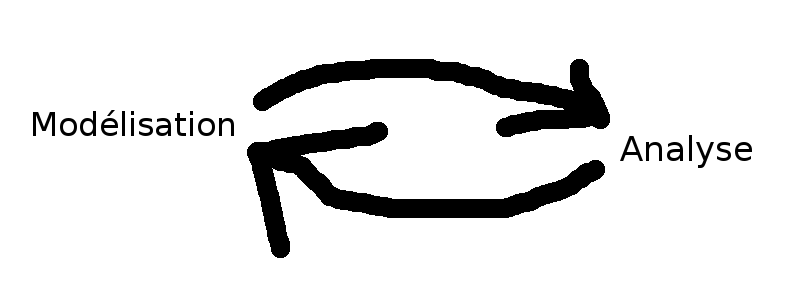
\includegraphics[width=.4\textwidth]{figs/modelanalyse.png}
\end{center}

L'analyse recherchée impacte les choix de modélisation
\begin{itemize}
  \item Les outils de modélisation doivent être adaptés aux propriétés observées
\end{itemize}

\medskip
Les choix de modélisation impactent les résultats de l'analyse
\begin{itemize}
  \item Un modèle trop grossier donne peu d'informations
  \item Un modèle de grande taille augmente le temps d'analyse
\end{itemize}

\medskip
\begin{center}
\tval{Les étapes de modélisation et d'analyse d'un système sont indissociables}
\end{center}

\end{frame}


\section{État de l'art de la modélisation}
% Abstractions

\begin{frame}[c]
  \frametitle{Abstractions de la représentation}

\begin{center}
  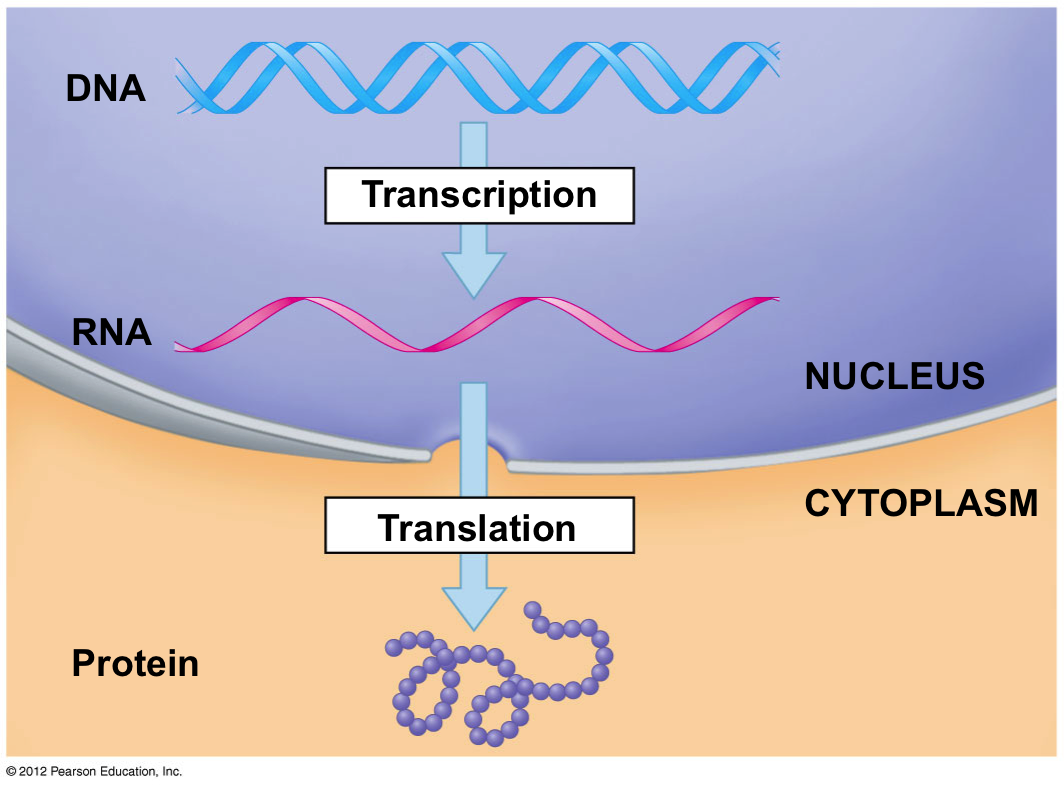
\includegraphics[width=.5\textwidth]{figs/protein.png}
  \uncover<2>{
    \begin{tikzpicture}
      \path[use as bounding box] (-3, 1) rectangle (0, -2);
      \node at (-1.5,.7) (ga) {\underline{Gène a}};
      \node at (-1.5,-0.7) (pa) {\underline{Protéine a}};
      \node[draw=none] at (-2.5,0) {$\Rightarrow$};
      \path[draw,->] (ga) -- (pa);
      \node[draw=none] at (-0.5,0) {$\Rightarrow$};
    \end{tikzpicture}}
  \uncover<2>{
    \scalebox{2}{
    \begin{tikzpicture}[adn]
      \path[use as bounding box] (-.3, .5) rectangle (0.5, -1);
      \node (a) {a};
    \end{tikzpicture}}
  }
\end{center}

\end{frame}



\begin{frame}[c]
  \frametitle{Discrétisation et asynchronisme}
  \framesubtitle{\tcite{\citerichard}}

\begin{center}
  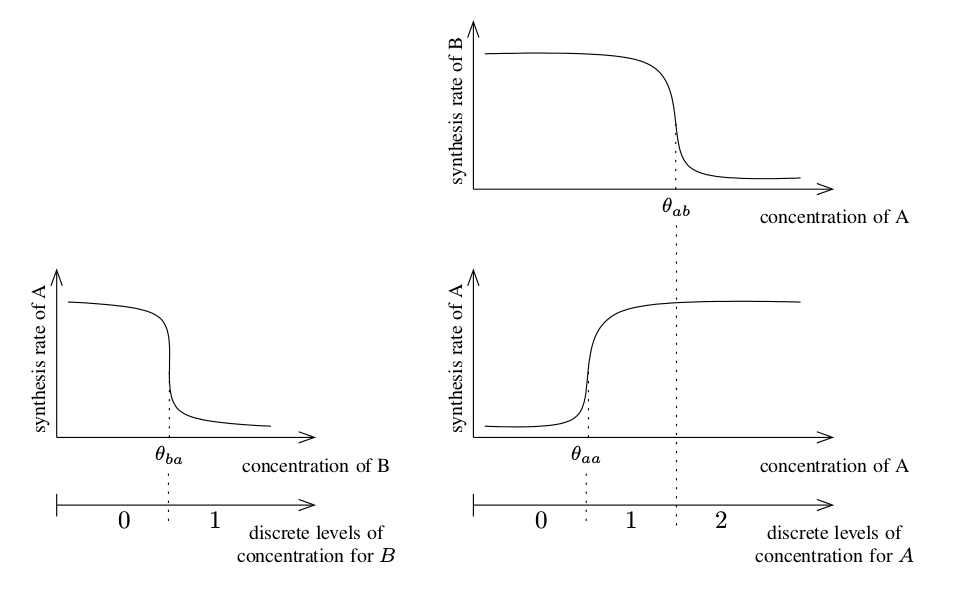
\includegraphics[width=.75\textwidth]{figs/seuils1.png}
\end{center}

\begin{tikzpicture}[adn]
  \path[use as bounding box] (-1.5,-5) rectangle (2.7,-5);
  
  \node[inner sep=0] (a) at (0,0) {a};
  \node[inner sep=0] (b) at (2,0) {b};
  
  \path node[elabel, below=-1em of b] {$\segm{0}{1}$};
  \path<2-> node[elabel, below=-1em of a] {$\segm{0}{2}$};
  
  \path<1> (b) edge[very thick,bend right=15] (a);
  \path<2-> (b) edge[bend right=15] (a);
  
  \path<2-> (a) edge[very thick,bend right=15] (b)
    (a) edge[very thick,loop left] (a);
  
  \path<1>[fill=white] (3.3,-4.2) rectangle (8,1);
\end{tikzpicture}

\vspace*{-2.5em}
\pause[3]
\begin{itemize}
  \item Concentrations ou niveaux d'activité continus\\
    \quad \f Abstraction sous forme de seuils et de \tval{niveaux discrets}
\pause
  \item Variations continues des valeurs réelles\\
    \quad \f Dynamique \tval{unitaire}
\pause
  \item Simultanéité de passage d'un seuil très peu probable\\
    \quad \f Dynamique \tval{asynchrone}
\end{itemize}

\end{frame}

% Définition du Réseaux Discrets Asynchrones

\newcommand{\Fadn}{\mathbb{F}}
\newcommand{\Eadn}{\mathbb{E}}
\newcommand{\SGadn}{\mathrm{G}}

\begin{frame}[t]
  \frametitle{Réseaux discrets / Modèle de Thomas}
  \framesubtitle{\todo{Citer Kauffman \& Thomas}}

\begin{itemize}
  \item Un ensemble de composants \qex{$N = \{ a, b, z \}$}
\uncover<2->{
  \item Un ensemble de niveaux d'expression pour chaque composant \qex{$z \in \Fadn^z = \segm{0}{2}$}
  \item L'ensemble des états globaux \qex{$\Fadn = \Fadn^a \times \Fadn^b \times \Fadn^z$}
}
\uncover<3->{
  \item Une fonction d'évolution pour chaque composant \qex{$f^z : \Fadn \rightarrow \Fadn^z$}
}
\uncover<4->{
  \item Signes et seuils sur les arcs \qex{$a \xrightarrow{+1}z$}
\end{itemize}
}

\uncover<3->{
\begin{center}
\begin{tabular}{ccc}
%  \ex{$f^a = \neg b$} & \ex{$f^b = b \vee \neg a$} & \ex{$f^z = a + b$} \vspace{.5em}\\
  \begin{tabular}[t]{c|c}
    $b$ & $f^a(b)$ \\
  \hline
    $0$ & $\mathbf{1}$ \\
    $1$ & $\mathbf{0}$ \\
  \end{tabular}
&
  \begin{tabular}[t]{cc|c}
    $a$ & $b$ & $f^b(a, b)$ \\
  \hline
    $0$ & $0$ & $\mathbf{1}$ \\
    $0$ & $1$ & $\mathbf{1}$ \\
    $1$ & $0$ & $\mathbf{0}$ \\
    $1$ & $1$ & $\mathbf{1}$
  \end{tabular}
&
  \begin{tabular}[t]{cc|c}
    $a$ & $b$ & $f^z(a, b)$ \\
  \hline
    $0$ & $0$ & $\mathbf{0}$ \\
    $0$ & $1$ & $\mathbf{1}$ \\
    $1$ & $0$ & $\mathbf{1}$ \\
    $1$ & $1$ & $\mathbf{2}$
  \end{tabular}
\end{tabular}
}

\bigskip

\begin{tikzpicture}[adn]
  \path[use as bounding box] (-0.7,-0.7) rectangle (2.5,2);
  \node[inner sep=0] (z) at (2,0.75) {z};
  \node[inner sep=0] (a) at (0,1.5) {a};
  \node[inner sep=0] (b) at (0,0) {b};
  \path<2->
    node[alabel, above=-1em of a] {$\segm{0}{1}$}
    node[alabel, below=-1em of b] {$\segm{0}{1}$}
    node[alabel, below=-1em of z] {$\segm{0}{2}$};
  \path<3->
    (a) edge[bend right=15] (b)
    (b) edge[bend right=15] (a)
    (b) edge[loop left] (b)
    (a) edge (z)
    (b) edge (z);
  \path<4->
    (a) edge[draw=none,bend right=15] node[alabel,left=-1pt] {$-1$} (b)
    (b) edge[draw=none,bend right=15] node[alabel,right=-3pt] {$+1$} (a)
    (b) edge[draw=none,loop left] node[alabel,left=-2pt] {$+1$} (b)
    (a) edge[draw=none] node[alabel,above=-2pt] {$+1$} (z)
    (b) edge[draw=none] node[alabel,below=-2pt] {$-1$} (z);
\end{tikzpicture}
\end{center}

\end{frame}



\begin{frame}[c]
  \frametitle{Analyse des modèles de Thomas}

Graphe des états: $\SGadn = (\Fadn, \Eadn)$, avec une dynamique asynchrone (et unitaire)\\
selon les fonctions d'évolution $f^a$ :
$$(x, y) \in \Eadn \Longleftrightarrow \exists a \in N, y^a = f^a(x) \wedge \forall b \neq a, y^b = x^b$$

%\f Only one component at a time $a$ evolves to reach the value of its evolution function $f^a(x)$

\pause
\medskip
%\begin{tabular*}{\textwidth}{@{\extracolsep{\fill}}lcc}
%  Size of the State Graph: & $\displaystyle|\Fadn| = \prod_{a \in N} |\Fadn^a| \quad\geq 2^{|N|}$ &
%\end{tabular*}
Taille du graphe des états: \quad $\displaystyle|\Fadn| = \prod_{a \in N} |\Fadn^a| \quad\geq 2^{|N|}$

\medskip
\f \tval{Exponentielle} dans le nombre $|N|$ de composants

\pause
\bigskip
Travaux permettant de tracer un lien entre structure et dynamique des modèles de Thomas :
\begin{itemize}
  \item \tval{Conjectures de Thomas'} (conditions pour cycles ou multi-stationnarité)
  \begin{itemize}
    \item Cas booléen : \tcite{\todo{citeremy}}
    \item Cas multivalué : \tcite{\todo{citerichardcomet}}
  \end{itemize}
\end{itemize}

\pause
\medskip
Mais les méthodes calculant l'atteignabilité nécessitent le graphe des états\\
Ex : \ex{Depuis l'état $(a, b, z) = (0, 0, 0)$, est-il possible d'atteindre $z = 2$ ?}
\begin{itemize}
  \item \tval{Logiques temporelles}
  \begin{itemize}
    \item CTL : \tcite{\todo{citesmbionet}}
    \item LTL : \tcite{\todo{citeito}}
  \end{itemize}
\end{itemize}
\end{frame}


% Définition du Process Hitting + sortes coopératives

\begin{frame}[c]
  \frametitle{Les Frappes de Processus standards}

Les \tval{Frappes de Processus standards} :
\begin{itemize}
  \item Adaptées à la représentation des RRB
  \item Modélisation \tval{atomique et qualitative} (niveaux discrets explicites)
  \item Dynamique \tval{simple mais puissante} (forme des actions contrainte)
\end{itemize}

\pause
\bigskip
Outils développés précédemment :
\begin{itemize}
  \item \tval{Analyse d'atteignabilité}
  \item Recherche de points fixes
  \item Paramètres stochastiques
\end{itemize}

\medskip
\f Formalisme bien adapté à l'étude des \tval{grands réseaux de régulation}

\pause
\bigskip
Quelques lacunes :
\begin{itemize}
  \item Représentation inexacte des \tval{coopérations}
  \item \tval{Enrichissement possible} de l'expressivité\\
    \quad \f Nécessité d'adapter les outils développés
\end{itemize}

\end{frame}



\begin{frame}[t]
  \frametitle{Les Frappes de Processus standards}
  \framesubtitle{\tcite{\cpmrtcsb}}

% 1 : Sortes
\only<1>{
\tikzstyle{process}=[circle,minimum size=15pt,font=\footnotesize,inner sep=1pt]
\tikzstyle{tick label}=[color=white, font=\footnotesize]
\tikzstyle{tick}=[transparent]
\tikzstyle{hit}=[transparent]
\tikzstyle{selfhit}=[transparent, min distance=30pt,curve to]
\tikzstyle{bounce}=[transparent]
\tikzstyle{hlhit}=[transparent]
\begin{center}\scalebox{\scaleex}{
\begin{tikzpicture}
  \exphdef
\end{tikzpicture}
}\end{center}
}

% 2 : Processus
\only<2>{
\tikzstyle{process}=[circle,draw,minimum size=15pt,font=\footnotesize,inner sep=1pt]
\tikzstyle{tick label}=[font=\footnotesize]
\tikzstyle{tick}=[densely dotted]
\tikzstyle{hit}=[transparent]
\tikzstyle{selfhit}=[transparent, min distance=30pt,curve to]
\tikzstyle{bounce}=[transparent]
\tikzstyle{hlhit}=[transparent]
\begin{center}\scalebox{\scaleex}{
\begin{tikzpicture}
  \exphdef
\end{tikzpicture}
}\end{center}
}

% 3 : États
\only<3>{
\tikzstyle{hit}=[transparent]
\tikzstyle{selfhit}=[transparent, min distance=30pt,curve to]
\tikzstyle{bounce}=[transparent]
\tikzstyle{hlhit}=[transparent]
\begin{center}\scalebox{\scaleex}{
\begin{tikzpicture}
  \exphdef

  \TState{3}{a_0,b_1,z_0}
\end{tikzpicture}
}\end{center}
}

% 4 : Actions
\only<4->{
\tikzstyle{tick}=[densely dotted]
\tikzstyle{hit}=[->,>=angle 45]
\tikzstyle{selfhit}=[min distance=30pt,curve to]
\tikzstyle{bounce}=[densely dotted,>=stealth',->]
\tikzstyle{hlhit}=[very thick]
\begin{center}\scalebox{\scaleex}{
\begin{tikzpicture}
\exphdef
  \TState{4-5}{a_0,b_1,z_0}
  \TState{6}{a_0,b_1,z_1}
  \TState{7}{a_1,b_1,z_1}
  \TState{8}{a_1,b_1,z_2}

  \only<5>{
    \THit{b_1}{hl}{z_0}{.west}{z_1}
    \path[bounce,bend left,hl] \TBounce{z_0}{}{z_1}{.south};
  }
  \only<6>{
    \THit{a_0}{out=250,in=200,selfhit,hl}{a_0}{.west}{a_1}
    \path[bounce,bend left,hl] \TBounce{a_0}{}{a_1}{.south};
  }
  \only<7>{
    \THit{a_1}{hl}{z_1}{.west}{z_2}
    \path[bounce,bend left,hl] \TBounce{z_1}{}{z_2}{.south};
  }
\end{tikzpicture}
}\end{center}
}

\medskip
\begin{liste}
  \item \tval{Sortes} : composants \qex{$a$, $b$, $z$}
\pause[2]
  \item \tval{Processus} : états locaux / niveaux d'expression \qex{$z_0$, $z_1$, $z_2$}
\pause[3]
  \item \tval{États} : ensembles de processus actifs%
  \only<3-5>{\qex{$\PHetat{a_0, b_1, z_0}$}}%
  \only<6>{\qex{$\PHetat{a_0, b_1, z_1}$}}%
  \only<7>{\qex{$\PHetat{a_1, b_1, z_1}$}}%
  \only<8>{\qex{$\PHetat{a_1, b_1, z_2}$}}%
\pause[4]
  \item \tval{Actions} : dynamique \qex{\only<5>{\underline}{$\PHfrappe{b_1}{z_0}{z_1}$}, \only<6>{\underline}{$\PHfrappe{a_0}{a_0}{a_1}$}, \only<7>{\underline}{$\PHfrappe{a_1}{z_1}{z_2}$}}
\end{liste}
\end{frame}



\begin{frame}
  \frametitle{Coopérations}
  \framesubtitle{\tcite{\cpmrtcsb}}

\begin{center}\scalebox{\scaleex}{
\begin{tikzpicture}
  \exphcoop
  
  \TState{9}{a_1,b_1}
  \TState{10}{a_1,b_1,ab_0}
  \TState{11}{a_1,b_1,ab_1}
  \TState{12}{a_1,b_1,ab_3}
  
  \node at (a_1.center) {\textasteriskcentered};
  \node at (b_1.center) {\textasteriskcentered};
  \node<5-> at (ab_3.center) {\textasteriskcentered};
  
  \only<9>{
    \node[hl process] at (ab_0.center) {};
    \node[hl process] at (ab_1.center) {};
    \node[hl process] at (ab_2.center) {};
    \node[current process] at (ab_3.center) {};
  }
  
  \only<10>{
    \THit{b_1}{hl}{ab_0}{.210}{ab_1}
    \path[bounce,bend left,hl] \TBounce{ab_0}{}{ab_1}{.240} ;
  }
  
  \only<11>{
    \THit{a_1}{hl}{ab_1}{.160}{ab_3}
    \path[bounce,bend left,hl] \TBounce{ab_1}{}{ab_3}{.south west} ;
  }
\end{tikzpicture}
}\end{center}

\medskip
\begin{liste}
  \item \tval{Coopération} entre \ex{$a_1$} et \ex{$b_1$} : \qex{$\PHfrappe{\underline{a_1 \wedge b_1}}{z_0}{z_1}$}
\pause[5]
  \item Solution : une \tval{sorte coopérative} \qex{$ab$} \quad pour exprimer \qex{$\underline{a_1 \wedge b_1}$}
\pause[9]
  \item Chaque configuration est représentée par un processus \qex{$\underline{a_1 \wedge b_1} \Rightarrow ab_{11}$}
%\pause[15]
%  \item Advantage: regular sort; drawbacks: complexity, temporal shift
\end{liste}
\end{frame}

% Présentation de l'analyse statique

\begin{frame}
  \frametitle{Approximations de l'analyse d'atteignabilité}
  \framesubtitle{\tcite{\cpmrmscs}}

Vérification des propriétés de la forme :
\begin{center}
  «~Depuis un état initial $s_0$, peut-on atteindre un état $s_n$ où $a_i$ est actif~?~»
\end{center}
Utilisation d'approximations $P$ et $Q$, telles que \tval{$P \Rightarrow R \Rightarrow Q$}

% Static analysis by abstractions:
% \begin{fleches}
%   \item Directly checking an objective sequence $R$ is hard
%   \item Rather check the approximations $P$ and $Q$, where \tval{$P \Rightarrow R \Rightarrow Q$}:
% \end{fleches}

\begin{center}
\scalebox{0.6}{
\begin{tikzpicture}
  \path[use as bounding box] (-5,-3.5) rectangle (5,3.5);
  \definecolor{r2}{RGB}{238,10,38}

  %\path<2->[shading=1, inner color=r2, outer color=white] (3.5,-2.8) -- (4.4,3.2) -- (0,3) -- (-4.5,1.4) -- (-2.5,-2.5) -- (0,-3.6) -- (2.8,-2.8);
  \draw<2->[shading=2, inner color=r2, outer color=white, rounded corners, draw=none] (-6,3.5) rectangle (6,-3.5);
  %\draw<2->[thick,fill=white] (2.5,-2.1) -- (3,2.5) -- (-2.7,1.3) -- (-2,-2) -- (2.5,-2.1);
  \draw<2->[thick,fill=white] (-2.8,2) rectangle (2.8,-2);
  %\draw<6->[thick,fill=lightyellow] (2.5,-2.1) -- (3,2.5) -- (-2.7,1.3) -- (-2,-2) -- (2.5,-2.1);
  \draw<6->[thick,fill=lightyellow] (-2.8,2) rectangle (2.8,-2);

  \node<2->[text width=3.5cm, color=red] (s1) at (-5,2) {Sur-approximation};
  \path<2->[->,very thick,color=red] (s1.south) edge (-3,1.2);
  \node<2->[text width=3cm,color=black] (q) at (2.2,2.3) {$\neg Q$};

  %\draw<4->[thick, shading=1, top color=darkgreen, bottom color=green] (.5,-.8) -- (1,0) -- (.3,1) -- (-1,.5) -- (-.5,-.5) -- (.5,-.8);
  \draw<4->[thick, shading=1, top color=darkgreen, bottom color=green] (-1.5,.7) rectangle (1.5,-.7);;
  \node<4->[text width=3.5cm,color=darkgreen] (s2) at (5.2,-2.5) {Sous-approximation};
  \node<4->[text width=3cm,color=black] (p) at (1.8,.4) {$P$};
  \path<4->[->,very thick,color=darkgreen] (s2) edge (1,-.8);

  \node[text width=3cm,align=center,color=darkcyan] (s) at (0,-1.7) {Solution exacte};
  \node<1->[text width=3cm,color=darkcyan] (s0) at (0,0) {};
  \draw[color=darkcyan, ultra thick] (0,0) ellipse (2 and 1.5);
  \node[text width=3cm,color=black] (r) at (2,1.2) {$R$};

  \only<3->{
    \node[point] at (-3.3,-1) {};
    \node[point] at (2,2.5) {};
  }
  \only<5->{
    \node[point] at (-1,.2) {};
    \node[point] at (1.1,-.5) {};
  }
  \only<7->{
    \node[point] at (-.5,-1.1) {};
    \node[point] at (2.5,1) {};
  }
\end{tikzpicture}
}
\end{center}

\uncover<8->{
Polynomial dans le nombre de sortes\\
Exponentiel dans le nombre de processus de chaque sorte
\begin{fleches}
  \item Efficace pour de grands modèles avec peu de niveaux d'expression
\end{fleches}
}
\end{frame}


\section{Enrichissement des Frappes de Processus}
\begin{frame}[t]
  \frametitle{The Metazoan Segmentation Model}
  \framesubtitle{\tcite{François \textit{et al.} in Molecular Systems Biology, 2007}}

\makenoprio

\begin{tikzpicture}
  \path[use as bounding box] (-1,0) rectangle (8,6.5);
  
  \draw<2>[very thick, darkgreen, fill=green!10] (7,4.5) ellipse [x radius=1cm,y radius=2cm];
  \node<2>[darkgreen, align=flush left, text width=3cm] at (7.7,2) {\Large \tval{Pigment production}};
  \draw<2> (8,4) node[anchor=west, darkgreen] {0 = inactive}
           (8,5) node[anchor=west, darkgreen] {1 = production};
  
  \draw<3>[very thick, darkred, fill=red!10] (0,4.7) ellipse [x radius=1cm,y radius=1.5cm];
  \node<3>[darkred, align=flush left, text width=2cm, anchor=west] at (1,5.8) {\Large \tval{Repression of $a$}};
  
  \draw<4>[very thick, darkviolet, fill=violet!10] (1,0.5) ellipse [x radius=1cm,y radius=1.5cm];
  \node<4>[darkviolet, align=flush left, anchor=west] at (2,-.3) {\Large \tval{Wavefront progression}};
  \draw<4> (0,0) node[anchor=east, darkviolet] {0 = “Off”}
           (0,1) node[anchor=east, darkviolet] {1 = “On”};
  
  \exmetazoan
  
  \only<-4>{
    \THit{f_1.north east}{selfhit, min distance=30, bend left, out=150, in=90}{f_1}{.south east}{f_0}
    \path[bounce, bend left=50]
      \TBounce{f_1}{}{f_0}{.north east};
  }
  
  \only<5>{
    \THit{f_1.north east}{selfhit, min distance=30, bend left, out=150, in=90,hlr}{f_1}{.south east}{f_0}
    \path[bounce, bend left=50]
      \TBounce{f_1}{hlr}{f_0}{.north east};
  }
  
  \only<-5>{
    \THit{f_0.east}{bend right=60, in=-140}{c_1}{.south east}{c_0}
    \path[bounce, bend left=50]
      \TBounce{c_1}{}{c_0}{.north east};
  }
  
  \only<6>{
    \THit{f_0.east}{bend right=60, in=-140, hlr}{c_1}{.south east}{c_0}
    \path[bounce, bend left=50]
      \TBounce{c_1}{hlr}{c_0}{.north east};
  }
  
  \only<7,13,24,26,28>{
    \THit{fc_2}{\prio, hl}{a_0}{.west}{a_1} \path[bounce, bend left=50, hl] \TBounce{a_0}{\prio}{a_1}{.south west};
  }
  \only<8,14,19,21,23,30>{
    \THit{f_1}{bend left=30, in=90, hl}{c_0}{.west}{c_1} \path[bounce, bend left=50, hl] \TBounce{c_0}{}{c_1}{.south west};
  }
  \only<9,12,15,18>{
    \path (0.8, 4.5) edge[\superprio,coopupdate,hl] (3.2, 3);
  }
  \only<10,16,25,27>{
    \THit{c_1}{\prio, hl}{a_1}{.west}{a_0} \path[bounce, bend right=50, hl] \TBounce{a_1}{\prio}{a_0}{.north west};
  }
  \only<11,17,20,22,29>{
    \THit{c_1}{selfhit, hl}{c_1}{.west}{c_0} \path[bounce, bend right=50, hl] \TBounce{c_1}{}{c_0}{.north west};
  }
  
  \TState{1-7,13,19}{f_1, a_0, c_0, fc_2}
  \TState{8,14}{f_1, a_1, c_0, fc_2}
  \TState{9,15}{f_1, a_1, c_1, fc_2}
  \TState{10,16}{f_1, a_1, c_1, fc_3}
  \TState{11,17}{f_1, a_0, c_1, fc_3}
  \TState{12,18}{f_1, a_0, c_0, fc_3}

  \TState{20,22,24}{f_1, a_0, c_1, fc_2}
  \TState{21,23}{f_1, a_0, c_0, fc_2}

  \TState{25,27,29,31}{f_1, a_1, c_1, fc_2}
  \TState{26,28}{f_1, a_0, c_1, fc_2}
  \TState{30}{f_1, a_1, c_0, fc_2}
\end{tikzpicture}

\pause[7]

\vspace*{-3cm}
\hfill
\begin{tikzpicture}

\tikz \foreach \x in {0,...,12}
  \draw[dotted] (\x/4,0) -- (\x/4,1.5);

\draw[dotted] (0,0) -- (-3,0);
\draw[dotted] (0,1.5) -- (-3,1.5);

\only<8->{\fill (-3,0) rectangle (-2.75,1.5);}
\only<9->{\fill (-2.75,0) rectangle (-2.5,1.5);}
\only<10->{\fill (-2.5,0) rectangle (-2.25,1.5);}
\only<11->{\fill[gray!30] (-2.25,0) rectangle (-2,1.5);}
\only<12->{\fill[gray!30] (-2,0) rectangle (-1.75,1.5);}
\only<13->{\fill[gray!30] (-1.75,0) rectangle (-1.5,1.5);}
\only<14->{\fill (-1.5,0) rectangle (-1.25,1.5);}
\only<15->{\fill (-1.25,0) rectangle (-1,1.5);}
\only<16->{\fill (-1,0) rectangle (-0.75,1.5);}
\only<17->{\fill[gray!30] (-0.75,0) rectangle (-0.5,1.5);}
\only<18->{\fill[gray!30] (-0.5,0) rectangle (-0.25,1.5);}
\only<19->{\fill[gray!30] (-0.25,0) rectangle (0,1.5);}

\end{tikzpicture}

\pause[15]
\vspace*{.5cm}
\hfill
\begin{tikzpicture}

\tikz \foreach \x in {0,...,12}
  \draw[dotted] (\x/4,0) -- (\x/4,1.5);

\draw[dotted] (0,0) -- (-3,0);
\draw[dotted] (0,1.5) -- (-3,1.5);

\only<20->{\fill[gray!30] (-3,0) rectangle (-2.75,1.5);}
\only<21->{\fill[gray!30] (-2.75,0) rectangle (-2.5,1.5);}
\only<22->{\fill[gray!30] (-2.5,0) rectangle (-2.25,1.5);}
\only<23->{\fill[gray!30] (-2.25,0) rectangle (-2,1.5);}
\only<24->{\fill[gray!30] (-2,0) rectangle (-1.75,1.5);}
\only<25->{\fill (-1.75,0) rectangle (-1.5,1.5);}
\only<26->{\fill[gray!30] (-1.5,0) rectangle (-1.25,1.5);}
\only<27->{\fill (-1.25,0) rectangle (-1,1.5);}
\only<28->{\fill[gray!30] (-1,0) rectangle (-0.75,1.5);}
\only<29->{\fill (-0.75,0) rectangle (-0.5,1.5);}
\only<30->{\fill (-0.5,0) rectangle (-0.25,1.5);}
\only<31->{\fill (-0.25,0) rectangle (0,1.5);}

\end{tikzpicture}

\pause[15]

\end{frame}



\subsection{Classes de priorités}
% Définition des priorités

\begin{frame}[c]
  \frametitle{Frappes de Processus avec classes de priorités}

\begin{tikzpicture}
  \path[use as bounding box] (-5.2,-4) rectangle (5.2,3.5);
  \planPHstandard
  \planPHp
  \planPHan[stillhidden]
  \planPHmult[stillhidden]
  \planPHcanonique[stillhidden]
\end{tikzpicture}

\end{frame}



\begin{frame}[t]
  \frametitle{Introduction de classes de priorités}
  \framesubtitle{\tcite{\cfpmrcsbio}}

\bigskip
\begin{itemize}
  \item À chaque action est associée une classe de priorité
  \item Une action n'est jouable que si aucune action plus prioritaire ne l'est
\end{itemize}

\medskip

\begin{center}
% \begin{tabular}{ccccc}
%   \hspace*{.3cm}\tikz \node[labelprio1] {$1$}; \hspace*{.3cm} &
%   \hspace*{.3cm}\tikz \node[labelprio2] {$2$}; \hspace*{.3cm} &
%   \hspace*{.3cm}\tikz \node[labelprio3] {$3$}; \hspace*{.3cm} &
%   \vspace*{.5em}\hspace*{.3cm}\raisebox{5pt}{\ldots}\hspace*{.3cm} &
%   \hspace*{.3cm}\tikz \node[labelprion] {$n$}; \hspace*{.3cm} \\\hline
%   \multicolumn{2}{l}{
%   \parbox{1.5cm}{\vspace*{.5em}plus haute\\priorité}} &
%   %\parbox{1cm}{~} &
%   \parbox{1cm}{~} &&
%   \parbox{1.5cm}{\vspace*{.5em}plus basse\\priorité}
% \end{tabular}
% \hspace*{-1em}
% \raisebox{2.2pt}{$\blacktriangleright$}

\begin{tabular}{*{5}{>{\centering}p{1cm}}}
  \tikz \node[labelprio1] {$1$}; &
  \tikz \node[labelprio2] {$2$}; &
  \tikz \node[labelprio3] {$3$}; &
  \raisebox{5pt}{\ldots} &
  \tikz \node[labelprion] {$n$};
\vspace*{.5em} \tabularnewline \hline
  \multicolumn{2}{l}{\parbox{1.5cm}{\vspace*{.5em}le plus\\prioritaire}} &&
  \multicolumn{2}{r}{\parbox{1.5cm}{\raggedleft\vspace*{.5em}le moins\\prioritaire}}
\end{tabular}
\hspace*{-1em}
\raisebox{2.2pt}{$\blacktriangleright$}

\bigskip

\only<2-3>{
\bigskip
\begin{tikzpicture}
  \path[use as bounding box] (-0.5,-0.5) rectangle (2.5,1.5);
  \TSort{(0,0)}{a}{2}{l}
  \TSort{(2,0)}{b}{2}{r}
  \THit{a_0}{}{b_0}{.west}{b_1}
  \THit{a_0}{out=-120,in=180,selfhit}{a_0}{.west}{a_1}
  \path[bounce]
  \TBounce{a_0}{bend left}{a_1}{.south}
  \TBounce{b_0}{bend left}{b_1}{.south}
  ;
  \TState{-2}{a_0,b_0}
  \TState{3-}{a_1,b_0}

  \node[labelprio1] at (-1.5,-0.5) {$1$};
  \node[labelprio2] at (1,0.25) {$2$};
\end{tikzpicture}

\bigskip

\f $b_1$ n'est \tval{jamais atteignable}
}
\end{center}

\only<4->{
\begin{itemize}
  \item Permet de modéliser des classes d'actions de vitesses similaires
\end{itemize}
\begin{center}
\begin{tabular}{*{5}{>{\centering}p{1cm}}}
  \tikz \node[labelprio1,labelstocha] {$A$}; &
  \tikz \node[labelprio2,labelstocha] {$B$}; &
  \tikz \node[labelprio3,labelstocha] {$C$}; &
  \raisebox{5pt}{\ldots} &
  \tikz \node[labelprion,labelstocha] {$N$};
\vspace*{.5em} \tabularnewline \hline
  \multicolumn{1}{r}{\parbox{1cm}{\hspace*{-1.7cm}\parbox{2.5cm}{\raggedleft\vspace*{.5em}\tval{instantanée}\\(non contrôlable)}}} &
  \multicolumn{2}{l}{\parbox{2cm}{\vspace*{.5em}\tval{très rapide}\\(contrôlable)}} &
  \multicolumn{2}{r}{\parbox{2cm}{\raggedleft\vspace*{.5em}\tval{très lente}\\~}}
\end{tabular}
\hspace*{-1em}
\raisebox{2.2pt}{$\blacktriangleright$}
\end{center}
}

\end{frame}

% Priorités dans Metazoan

\begin{frame}[t]
  \frametitle{Metazoan Segmentation with Priorities}
  \framesubtitle{\tcite{\cfpmrcsbio}}

\makenoprio

\begin{tikzpicture}
  \path[use as bounding box] (-2,0) rectangle (8,6.5);
  \exmetazoan

  \node[labelprio1] at (2,3.3) {$1$};
  \node[labelprio1] at (2.3,1.6) {$1$};
  \node[labelprio2] at (5.5,3.9) {$2$};
  \node[labelprio2] at (3.5,5.3) {$2$};
  \node[labelprio3] at (0,2.5) {$3$};
  \node[labelprio3] at (0.8,5.8) {$3$};
  
  \TState{3,9,15}{f_1, a_0, c_0, fc_2}
  \TState{4,10}{f_1, a_1, c_0, fc_2}
  \TState{5,11}{f_1, a_1, c_1, fc_2}
  \TState{6,12}{f_1, a_1, c_1, fc_3}
  \TState{7,13}{f_1, a_0, c_1, fc_3}
  \TState{8,14}{f_1, a_0, c_0, fc_3}
\end{tikzpicture}

\pause[2]
\vspace*{-2.5cm}
\hfill
\begin{tikzpicture}
  \tikz \foreach \x in {0,...,12}
    \draw[dotted] (\x/4,0) -- (\x/4,1.5);

  \draw[dotted] (0,0) -- (-3,0);
  \draw[dotted] (0,1.5) -- (-3,1.5);

  \only<4->{\fill (-3,0) rectangle (-2.75,1.5);}
  \only<5->{\fill (-2.75,0) rectangle (-2.5,1.5);}
  \only<6->{\fill (-2.5,0) rectangle (-2.25,1.5);}
  \only<7->{\fill[gray!30] (-2.25,0) rectangle (-2,1.5);}
  \only<8->{\fill[gray!30] (-2,0) rectangle (-1.75,1.5);}
  \only<9->{\fill[gray!30] (-1.75,0) rectangle (-1.5,1.5);}
  \only<10->{\fill (-1.5,0) rectangle (-1.25,1.5);}
  \only<11->{\fill (-1.25,0) rectangle (-1,1.5);}
  \only<12->{\fill (-1,0) rectangle (-0.75,1.5);}
  \only<13->{\fill[gray!30] (-0.75,0) rectangle (-0.5,1.5);}
  \only<14->{\fill[gray!30] (-0.5,0) rectangle (-0.25,1.5);}
  \only<15->{\fill[gray!30] (-0.25,0) rectangle (0,1.5);}
\end{tikzpicture}

\pause[15]
%\vspace*{.3cm}
\begin{flushright}
  \f Only one\\possible behavior
\end{flushright}


\end{frame}



\begin{frame}[c]
  \frametitle{Metazoan Segmentation in Canonical Form}

\makenoprio

\vspace*{.5cm}
\scalebox{.9}{
\begin{tikzpicture}
  \path[use as bounding box] (-5.75,0) rectangle (5.75,5.5);
  \TSort{(-5,4)}{c}{2}{l}
  \TSort{(0,1)}{f}{2}{l}
  \TSort{(5,4)}{a}{2}{r}

  \TSetTick{fc}{0}{00}
  \TSetTick{fc}{1}{01}
  \TSetTick{fc}{2}{10}
  \TSetTick{fc}{3}{11}
  \TSort{(3,0)}{fc}{4}{r}
  
  \THit{fc_2}{}{a_0}{.south west}{a_1}
  \path[bounce, bend left=60]
    \TBounce{a_0}{}{a_1}{.south west};
  
  \THit{c_1.north east}{}{a_1}{.west}{a_0}
  \path[bounce, bend right=50]
    \TBounce{a_1}{}{a_0}{.north west};
  
  \path (0.8, 1.5) edge[\prio,coopupdate] (2.2, 1.5);
  \path (-4.3, 4.5) edge[\prio,coopupdate] (2.2, 2.5);
  
  \only<1>{
    \THit{c_1.north}{selfhit}{c_1}{.west}{c_0}
    \path[bounce, bend right=50]
      \TBounce{c_1}{}{c_0}{.north west};
  }
  
  \only<2>{
    \THit{c_1.north}{selfhit,hlr}{c_1}{.west}{c_0}
    \path[bounce, bend right=50]
      \TBounce{c_1}{hlr}{c_0}{.north west};
  }
  
  \only<-2>{
    \node[labelprio3] at (-4.4,6) {$3$};
  }
  
  \only<3>{
    \THit{a_0.west}{hlv}{c_1}{.east}{c_0}
    \path[bounce, bend left=50]
      \TBounce{c_1}{hlv}{c_0}{.north east};
    \node[labelprio2] at (0.5,4.7) {$2$};
  }
  
  \only<4->{
    \THit{a_0.west}{}{c_1}{.east}{c_0}
    \path[bounce, bend left=50]
      \TBounce{c_1}{}{c_0}{.north east};
    \node[labelprio2] at (0.5,4.7) {$2$};
  }
  
  \only<-4>{
    \node[labelprio3] at (-3,2.3) {$3$};
  }
  
  \only<-3>{
    \THit{f_1}{bend left=30, in=90}{c_0}{.west}{c_1}
    \path[bounce, bend left=50]
      \TBounce{c_0}{}{c_1}{.south west};
  }
  
  \only<4>{
    \THit{f_1}{bend left=30, in=90, hlr}{c_0}{.west}{c_1}
    \path[bounce, bend left=50]
      \TBounce{c_0}{hlr}{c_1}{.south west};
  }
  
  \only<5->{
    \TSetTick{fa}{0}{00}
    \TSetTick{fa}{1}{01}
    \TSetTick{fa}{2}{10}
    \TSetTick{fa}{3}{11}
    \TSort{(-3,0)}{fa}{4}{l}
    
    \path (-0.8, 1.5) edge[\prio,coopupdate] (-2.2, 1.5);
    \path (4.3, 4.5) edge[\prio,coopupdate] (-2.2, 2.5);
    
    \only<5>{
      \THit{fa_3}{hlv}{c_0}{.east}{c_1}
      \path[bounce, bend right=50]
        \TBounce{c_0}{hlv}{c_1}{.south east};
    }
    
    \only<6->{
      \THit{fa_3}{}{c_0}{.east}{c_1}
      \path[bounce, bend right=50]
        \TBounce{c_0}{}{c_1}{.south east};
    }
  
    \node[labelprio1] at (-1.5,3) {$1$};
    \node[labelprio1] at (-1.5,1.8) {$1$};
    \node[labelprio2] at (-4,3.85) {$2$};
  }
  
  \node[labelprio1] at (1.5,3) {$1$};
  \node[labelprio1] at (1.5,1.8) {$1$};

  \node[labelprio2] at (0,5.4) {$2$};
  \node[labelprio2] at (4.4,3) {$2$};
\end{tikzpicture}
}

\pause[6]
\vspace{.7cm}
\begin{center}
  \f Same dynamics but only 2 priorities
  
  \f Priority \raisebox{-2pt}{\tikz \node[labelprio1] {$1$};} is only for cooperative sorts
\end{center}

\end{frame}

\subsection{Arcs neutralisants}
% Arcs neutralisants

\begin{frame}[c]
  \frametitle{Frappes de Processus avec arcs neutralisants}

\begin{tikzpicture}
  \path[use as bounding box] (-5.2,-4) rectangle (5.2,3.5);
  \planPHstandard
  \planPHp
  \planPHan
  \planPHmult[stillhidden]
  \planPHcanonique[stillhidden]
\end{tikzpicture}

\end{frame}



\begin{frame}[c]
  \frametitle{Arcs neutralisants}

\begin{columns}
\begin{column}{.4\textwidth}

\begin{tikzpicture}
  %\path[use as bounding box] (-2,0) rectangle (8,6.5);
  \TSort{(0,0)}{a}{2}{l}
  \TSort{(2,0)}{b}{2}{r}
  \TSort{(0,3)}{c}{2}{l}
  \TSort{(2,3)}{d}{2}{r}
  
  \THit{a_0}{}{b_0}{.west}{b_1}
  \path[bounce] \TBounce{b_0}{bend left}{b_1}{.south};
  
  \THit{c_0}{}{d_0}{.west}{d_1}
  \path[bounce] \TBounce{d_0}{bend left}{d_1}{.south};
  
  \node (nea1) at (1,0) {};
  \node[dotne] (nea2) at (1,2.9) {};
  \draw[linene] (nea1) to[out=100, in=-100] (nea2);
  
  \TState{1}{a_0, b_0, c_0, d_0}
  \TState{2}{a_0, b_1, c_0, d_0}
  \TState{3}{a_0, b_1, c_0, d_1}
\end{tikzpicture}

\end{column}
\begin{column}{.55\textwidth}
\begin{center}

\begin{itemize}
  \item Intégration de données temporelles\\
    concernant les temps de réaction relatifs
  \item Préemptions atomiques entre les actions\\
    similaires à des «~priorités atomiques~»
\end{itemize}

\vspace*{1cm}
$\PHfrappe{c_0}{d_0}{d_1}$ ne peut être jouée \tval{tant que}

\bigskip
$\PHfrappe{a_0}{b_0}{b_1}$ est jouable

\bigskip
\f $d_1$ est \tval{toujours} atteint après $b_1$

\end{center}
\end{column}
\end{columns}


\end{frame}

% Arcs neutralisants sur Metazoan

\begin{frame}[t]
  \frametitle{Metazoan Segmentation with Neutralizing Edges}

\makenoprio

\begin{tikzpicture}
  \path[use as bounding box] (-2,0) rectangle (8,6.5);
  \exmetazoan

  \node (nea1) at (3.5,5) {};
  \node[dotne] (nea2) at (0.6,5.9) {};
  \draw[linene] (nea1) to[out=120, in=20] (nea2);

  \node (neb1) at (5.8,3.6) {};
  \node[dotne] (neb2) at (-0.5,2.5) {};
  \draw[linene] (neb1) to[out=-70, in=250, min distance=160] (neb2);
\end{tikzpicture}

\end{frame}

\subsection{Actions plurielles}
% Actions plurielles

\begin{frame}[c]
  \frametitle{Frappes de Processus avec actions plurielles}

\begin{tikzpicture}
  \path[use as bounding box] (-5.2,-4) rectangle (5.2,3.5);
  \planPHstandard
  \planPHp
  \planPHan
  \planPHmult
  \planPHcanonique[stillhidden]
\end{tikzpicture}

\end{frame}



\begin{frame}[c]
  \frametitle{Introduction d'actions plurielles}

\begin{columns}
\begin{column}{.4\textwidth}

\begin{tikzpicture}
  %\path[use as bounding box] (-2,0) rectangle (8,6.5);
  %\TSort{(0,0)}{b}{2}{l}
  \TSort{(0,2)}{y}{2}{l}
  \TSort{(3,0)}{z}{2}{r}
  \TSort{(3,3)}{x}{2}{r}
  
  \TActionPlur{y_1}{x_1.west}{x_0.north west}{}{1.5,2.5}{right}
  \TActionPlur{}{z_0.west}{z_1.south west}{}{1.5,2.5}{left}
  \TActionPlur{}{x_0.east}{x_1.south east}{}{4,2.5}{right}

  \TState{1}{x_1, y_1, z_0}
  \TState{2}{x_0, y_1, z_1}
  \TState{3}{x_1, y_1, z_1}
\end{tikzpicture}

\end{column}
\begin{column}{.55\textwidth}
\begin{center}

\begin{itemize}
  \item Synchronisations entre les actions :
  \begin{itemize}
    \item[--] Présence conjointe de réactifs
    \item[--] Consommation simultanée d'éléments
    \item[--] Production simultanée
  \end{itemize}
  \item Représentation d'équations biochimiques :\\
    \centering $X \xrightarrow{Y} Z$\\
    \raggedright sous la forme :\\
    \centering $h_2 = \PHfrappemults{x_1, y_1, z_0}{x_0, z_1}$\\
\end{itemize}

% \vspace*{.5cm}

% \ex{%
% $h_2 = \PHfrappemults{x_1, y_1, z_0}{x_0, z_1}$\\
% $h_1 = \PHfrappemults{c_0}{c_1}$%
% }

\vspace*{.5cm}
Tous les processus de $A$\\
doivent être présents pour jouer $\PHfrappemult{A}{B}$

\medskip
Après le jeu de $\PHfrappemult{A}{B}$,\\
tous les processus de $B$ sont présents
% 
% est jouable dans $s$ si et seulement si :
% 
% $A \subset s$
% 
% \bigskip
% Après jeu : $s \play (\PHfrappemult{A}{B}) = s \Cap B$

\end{center}
\end{column}
\end{columns}


\end{frame}

% Actions plurielles sur Metazoan

\begin{frame}[t]
  \frametitle{Utilisation des actions plurielles}

\makenoprio

\begin{tikzpicture}[apdotsimple/.style={apdot}]
  \path[use as bounding box] (-3,1) rectangle (6,6.5);
  \TSort{(0,4)}{c}{2}{l}
  \TSort{(1,0)}{f}{2}{l}
  \TSort{(5,4)}{a}{2}{r}

  \TActionPlur{f_1, c_0}{a_0.west}{a_1.south west}{}{2.5,2.5}{left}
%   \THit{fc_2}{\prio}{a_0}{.west}{a_1}
%   \path[bounce, bend left=50]
%     \TBounce{a_0}{\prio}{a_1}{.south west};
  
  \THit{c_1}{\prio}{a_1}{.west}{a_0}
  \path[bounce, bend right=50]
    \TBounce{a_1}{\prio}{a_0}{.north west};
  
  \THit{f_1}{bend left=30, in=90}{c_0}{.west}{c_1}
  \path[bounce, bend left=50]
    \TBounce{c_0}{}{c_1}{.south west};
  
  \TActionPlur{}{c_1.west}{c_0.north west}{}{-1,6}{right}
%   \THit{c_1}{selfhit}{c_1}{.west}{c_0}
%   \path[bounce, bend right=50]
%     \TBounce{c_1}{}{c_0}{.north west};
\end{tikzpicture}

\begin{flushright}
  \f Même dynamique qu'avec des priorités,\\
  à la sorte coopérative absente près.
\end{flushright}

\end{frame}


\section{Frappes de Processus canoniques et analyse}
\subsection{Frappes de Processus canoniques}
% Ajout des actions prioritaires pour avoir une équivalence avec les ADN

% \begin{frame}[t]
%   \frametitle{Adding cooperations}
%   \framesubtitle{\tcite{\cpmrtcsb}}
% 
% \begin{center}\scalebox{\scaleex}{
% \begin{tikzpicture}
%   \exphcoop
%   
%   \TState{9}{a_1,b_1}
%   \TState{10}{a_1,b_1,ab_0}
%   \TState{11}{a_1,b_1,ab_1}
%   \TState{12}{a_1,b_1,ab_3}
%   
%   \only<9>{
%     \node[hl process] at (ab_0.center) {};
%     \node[hl process] at (ab_1.center) {};
%     \node[hl process] at (ab_2.center) {};
%     \node[current process] at (ab_3.center) {};
%   }
%   
%   \only<10>{
%     \THit{b_1}{hl}{ab_0}{.210}{ab_1}
%     \path[bounce,bend left,hl] \TBounce{ab_0}{}{ab_1}{.240} ;
%   }
%   
%   \only<11>{
%     \THit{a_1}{hl}{ab_1}{.160}{ab_3}
%     \path[bounce,bend left,hl] \TBounce{ab_1}{}{ab_3}{.south west} ;
%   }
% \end{tikzpicture}
% }\end{center}
% 
% \medskip
% %\only<-14>{
% \begin{liste}
%   \item \tval{Cooperation} between \ex{$a_1$} and \ex{$b_1$}: \qex{$\PHfrappe{\underline{a_1 \wedge b_1}}{z_0}{z_1}$}
% \pause[5]
%   \item Solution: a \tval{cooperative sort} \qex{$ab$} \quad to express \qex{$\underline{a_1 \wedge b_1}$}
% \pause[9]
%   \item Constraint: each configuration is represented by one process \qex{$\underline{a_1 \wedge b_1} \Rightarrow ab_{11}$}
% %\pause[15]
% %  \item Advantage: regular sort; drawbacks: complexity, temporal shift
% \end{liste}%}
% \end{frame}



\begin{frame}[t]
  \frametitle{Adapting the expressivity of PH}
  \framesubtitle{\tcite{\cfpmrcsbio}}

\begin{center}\scalebox{\scaleex}{
\begin{tikzpicture}
  \path[use as bounding box] (-0.5,-0.5) rectangle (6.5,4.5);
  %\path[use as bounding box] (-1,-0.5) rectangle (7.5,5);

  \exphcoopprio{unprio}{}

  \node<5->[process,very thick] at (z_1.center) {?};

  \only<2>{
    \THit{a_1}{selfhit,hlb}{a_1}{.west}{a_0}
    \path[bounce,bend right,hlb] \TBounce{a_1}{}{a_0}{.north west} ;
  }
  \only<3>{
    \THit{b_0.south west}{bend left=90,hlb}{a_0}{.west}{a_1}
    \path[bounce,bend left,hlb] \TBounce{a_0}{}{a_1}{.south west} ;
  }
  \only<4>{
    \THit{b_1}{selfhit,hlb}{b_1}{.west}{b_0}
    \THit{a_0}{bend right=50,hlb}{b_0}{.west}{b_1}
    \path[bounce,bend right,hlb] \TBounce{b_1}{}{b_0}{.north west} ;
    \path[bounce,bend left,hlb] \TBounce{b_0}{}{b_1}{.south west} ;
  }

  \TState{5-6}{a_0, b_0, ab_0, z_0}
  \only<6>{
  \THit{b_0.south west}{hl,bend left=90}{a_0}{.west}{a_1}
  \path[bounce,bend left,hl] \TBounce{a_0}{}{a_1}{.south west} ;
  }
  \TState{7}{a_1, b_0, ab_0, z_0}
  \only<7>{
  \THit{a_1}{hl}{ab_0}{.west}{ab_2}
  \path[bounce,bend left,hl] \TBounce{ab_0}{}{ab_2}{.240} ;
  }
  \TState{8}{a_1, b_0, ab_2, z_0}
  \only<8>{
  \THit{a_1}{selfhit,hl}{a_1}{.west}{a_0}
  \path[bounce,bend right,hl] \TBounce{a_1}{}{a_0}{.north west} ;
  }
  \TState{9}{a_0, b_0, ab_2, z_0}
  \only<9>{
  \THit{a_0}{bend right=50,hl}{b_0}{.west}{b_1}
  \path[bounce,bend left,hl] \TBounce{b_0}{}{b_1}{.south west} ;
  }
  \TState{10}{a_0, b_1, ab_2, z_0}
  \only<10>{
  \THit{b_1}{hl}{ab_2}{.200}{ab_3}
  \path[bounce,bend left,hl] \TBounce{ab_2}{}{ab_3}{.south} ;
  }
  \TState{11}{a_0, b_1, ab_3, z_0}
  \only<11>{
  \THit{ab_3}{hl}{z_0}{.west}{z_1}
  \path[bounce,bend left,hl] \TBounce{z_0}{}{z_1}{.south} ;
  }
  \TState{12-}{a_0, b_1, ab_3, z_1}
\end{tikzpicture}
}\end{center}

\medskip

\tval{Drawback}: Cooperations are too “loose” to be as expressive as ADN.

\medskip

$ \uncover<5->{\PHstate{a_0, b_0, ab_{00}, z_0}}
  \uncover<7->{\rightarrow\PHstate{a_1, b_0, ab_{00}, z_0}}
  \uncover<8->{\rightarrow\PHstate{a_1, b_0, ab_{10}, z_0}}
  \uncover<9->{\rightarrow\PHstate{a_0, b_0, ab_{10}, z_0}}$
\\ \qquad
$ \uncover<10->{\rightarrow\PHstate{a_0, b_1, ab_{10}, z_0}}
  \uncover<11->{\rightarrow\PHstate{a_0, b_1, \redex{ab_{11}}, z_0}}
  \uncover<12->{\rightarrow\PHstate{a_0, b_1, \redex{ab_{11}}, \redex{z_1}}}$

\medskip

\uncover<12->{
The cooperativity should be: \qex{$a_1 \wedge b_1$~\tval{simultaneously}} \quad \textit{i.e.} “in the same state”

\smallskip
but the model behaves like: \qex{$\mathbf{P}(a_1) \wedge \mathbf{P}(b_1)$} \quad with $\mathbf{P}$ = “previously”
}
\end{frame}


\begin{frame}[t]
  \frametitle{Adapting the expressivity of PH}
  \framesubtitle{\tcite{\cfpmrcsbio}}

\begin{center}\scalebox{\scaleex}{
\begin{tikzpicture}
  \path[use as bounding box] (-0.5,-0.5) rectangle (6.5,4.5);

  \draw[draw=none, fill=blue!15] (2,2.1) ellipse (15pt and 2cm);
  \draw[draw=none, fill=red!15] (-1,2) ellipse (22pt and 10pt);
  \exphcoopprio{prio}{}
  \node[labelprio1] at (2,3.7) {$1$};
  
  \node[labelprio2] at (-.9,4.7) {$2$};  % a 1 -> a 1 0
  \node[labelprio2] at (-1.4,2) {$2$};  % b 0 -> a 0 1
%  \node[labelprio2] at (.7,2) {$2$};  % b 1 -> b 1 0
  \node[labelprio2] at (5.8,2.6) {$2$};  % ab 11 -> z 0 1

  \node[process,very thick] at (z_1.center) {?};

  \TState{3}{a_0, b_0, ab_0, z_0}
  \only<3>{
  \THit{b_0.south west}{hl,bend left=90}{a_0}{.west}{a_1}
  \path[bounce,bend left,hl] \TBounce{a_0}{}{a_1}{.south west} ;
  }
  \TState{4}{a_1, b_0, ab_0, z_0}
  \only<4>{
  \THit{a_1}{prio,hl}{ab_0}{.west}{ab_2}
  \path[bounce,bend left,hl] \TBounce{ab_0}{}{ab_2}{.240} ;
  }
  \TState{5}{a_1, b_0, ab_2, z_0}
  \only<5>{
  \THit{a_1}{selfhit,hl}{a_1}{.west}{a_0}
  \path[bounce,bend right,hl] \TBounce{a_1}{}{a_0}{.north west} ;
  }
  \TState{6}{a_0, b_0, ab_2, z_0}
  \only<6>{
  \THit{a_0}{prio,hl}{ab_2}{.160}{ab_0}
  \path[bounce,bend right,hl] \TBounce{ab_2}{}{ab_0}{.north west} ;
  }
  \TState{7}{a_0, b_0, ab_0, z_0}
  \only<7>{
  \THit{a_0}{bend right=50,hl}{b_0}{.west}{b_1}
  \path[bounce,bend left,hl] \TBounce{b_0}{}{b_1}{.south west} ;
  }
  \TState{8}{a_0, b_1, ab_0, z_0}
  \only<8>{
  \THit{b_1}{prio,hl}{ab_0}{.210}{ab_1}
  \path[bounce,bend left] \TBounce{ab_0}{hl}{ab_1}{.240} ;
  }
  \TState{9-}{a_0, b_1, ab_1, z_0}
\end{tikzpicture}
}\end{center}

\begin{itemize}
  \item Prioritise actions updating cooperative sorts (non-biological actions)
  \item All other actions remain unprioritised (evolutions with delays)
\end{itemize}
\pause
$\Rightarrow$ Whenever a regular action is played, all cooperative sorts are already updated

%\medskip
%Now, $z_1$ cannot be reached from $\PHstate{a_0, b_0, ab_{00}, z_0}$

\medskip
$ \uncover<3->{\PHstate{a_0, b_0, ab_{00}, z_0}}
  \uncover<4->{\rightarrow\PHstate{a_1, b_0, ab_{00}, z_0}}
  \uncover<5->{\rightarrow\PHstate{a_1, b_0, ab_{10}, z_0}}
  \uncover<6->{\rightarrow\PHstate{a_0, b_0, ab_{10}, z_0}}$
\\ \qquad
$ \uncover<7->{\rightarrow\PHstate{a_0, b_0, \ex{ab_{00}}, z_0}}
  \uncover<8->{\rightarrow\PHstate{a_0, b_1, \ex{ab_{00}}, z_0}}
  \uncover<9->{\rightarrow\PHstate{a_0, b_1, \ex{ab_{01}}, z_0}}$
\end{frame}

\subsection{Analyse statique}
% Analyse statique avec priorités

\begin{frame}[c]
  \frametitle{Analyse statique des Frappes de Processus canoniques}
  \framesubtitle{\tcite{\cfpmrcsbio}}
%  \framesubtitle{\tcite{\cpmrmscs}}

L'ajout de priorités restreint les dynamiques possibles (préemptions)

\smallskip
\f Invalidation de la sous-approximation existante

\begin{center}
\scalebox{0.6}{
\begin{tikzpicture}
  \path[use as bounding box] (-5,-3.5) rectangle (5,3.5);
  \definecolor{r2}{RGB}{238,10,38}

  \draw[shading=2, inner color=r2, outer color=white, rounded corners, draw=none] (-6,3.5) rectangle (6,-3.5);
  \draw[thick,fill=white] (-2.8,2) rectangle (2.8,-2);
  \draw<4->[thick,fill=lightyellow] (-2.8,2) rectangle (2.8,-2);
  \draw<1>[thick, shading=1, top color=darkgreen, bottom color=green,opacity=1] (-1.5,.7) rectangle (1.5,-.7);;
  \draw<2>[thick, shading=1, top color=darkgreen, bottom color=green,opacity=0.3] (-1.5,.7) rectangle (1.5,-.7);;
%  \draw<1>[color=darkcyan, ultra thick] (0,0) ellipse (2 and 1.5);
  \draw<1>[color=darkcyan, ultra thick] (1,1.3) arc [start angle=60, end angle=420, x radius=2, y radius=1.5] -- cycle;
  \draw<2->[color=darkcyan, ultra thick] (1,1.3) arc [start angle=60, end angle=300, x radius=2, y radius=1.5] -- cycle;
  \draw<3->[thick, shading=1, top color=darkgreen, bottom color=green] (-1.5,.7) rectangle (.8,-.7);;
\end{tikzpicture}
}
\end{center}

\uncover<5->{
Complexité équivalente pour un formalisme plus expressif

\begin{fleches}
  \item Toujours efficace pour de grands modèles
  \item Sous-approximation plus fine
\end{fleches}
}
\end{frame}


\begin{frame}[c]
  \frametitle{Analyse statique des Frappes de Processus canoniques}
  \framesubtitle{\tcite{\cfpmrcsbio}}

\uncover<8->{
\tval{Condition suffisante :}

\begin{itemize}
  \item aucun cycle
  \item tout objectif possède une solution
  \item \only<-11>{cohérence des coopérations}\only<12->{\sout{cohérence des coopérations}}
\end{itemize}
\vspace{1cm}
\hspace{2cm}\uncover<12->{\textcolor{darkyellow}{\textbf{Non conclusif}}}
\vspace{-3cm}
}

\begin{center}\scalebox{\scaleex}{
\begin{tikzpicture}[aS]
  \path[draw=none,use as bounding box] (-.5,-2.2) rectangle (12,2.2);
  \node[Aproc] (z1) {$z_1$};
  \uncover<2->{ \node[Aobj,right of=z1] (z01) {$\PHobj{z_0}{z_1}$}; }
  \uncover<3->{ \node[Asol,right of=z01] (z01s) {}; }
  
  \uncover<4->{ \node[Aproc,right of=z01s] (ab11) {$ab_{11}$}; }
  \uncover<5->{ \node[Asol,right of=ab11] (ab11s) {}; }
  
  \uncover<6->{
    \node[Aproc,above right of=ab11s] (a1) {$a_1$};
    \node[Aproc,below right of=ab11s] (b1) {$b_1$};
  }
  
  \uncover<7->{
    \node[Aobj,above right of=a1] (a11) {$\PHobj{a_1}{a_1}$};
    \node[Asol,right of=a11] (a11s) {};
    \node[Aobj,right of=a1] (a01) {$\PHobj{a_0}{a_1}$};
    \node[Asol,right of=a01] (a01s) {};
    \node[Aproc,right of=a01s] (b0) {$b_0$};
    \node[Aobj,right of=b0] (b00) {$\PHobj{b_0}{b_0}$};
    \node[Asol,right of=b00] (b00s) {};
    \node[Aobj,above right of=b0] (b10) {$\PHobj{b_1}{b_0}$};
    \node[Asol,right of=b10] (b10s) {};
    
    \node[Aobj,below right of=b1] (b11) {$\PHobj{b_1}{b_1}$};
    \node[Asol,right of=b11] (b11s) {};
    \node[Aobj,right of=b1] (b01) {$\PHobj{b_0}{b_1}$};
    \node[Asol,right of=b01] (b01s) {};
    \node[Aproc,right of=b01s] (a0) {$a_0$};
    \node[Aobj,right of=a0] (a00) {$\PHobj{a_0}{a_0}$};
    \node[Asol,right of=a00] (a00s) {};
    \node[Aobj,below right of=a0] (a10) {$\PHobj{a_1}{a_0}$};
    \node[Asol,right of=a10] (a10s) {};
  }
  
  \path (z1) edge (z01);
  \path<2-> (z01) edge (z01s);
  \path<3-> (z01s) edge (ab11);
  \path<4-> (ab11) edge[aSPrio] (ab11s);
  \path<5-> (ab11s) edge (a1) edge (b1);
  \path<6-> (a1) edge (a01) edge (a11) (b1) edge (b01) edge (b11);
  
  \path<7->
  (a01) edge (a01s)
  (a01s) edge (b0)
  (a11) edge (a11s)
  (a0) edge (a10) edge (a00)
  (a10) edge (a10s)
  (a00) edge (a00s)
  
  (b0) edge (b10) edge (b00)
  (b10) edge (b10s)
  (b00) edge (b00s)
  (b01) edge (b01s)
  (b01s) edge (a0)
  (b11) edge (b11s)
  ;
  
  % Arc non cohérent
  \node<9-11>[Aproc,Aex,at=(ab11)] {$ab_{11}$};
  \node<9-11>[Asol,Aexsol,right of=ab11] (ab11s) {};
  \path<9-11> (ab11) edge[aSPrio,Aexedge] (ab11s);
  \node<12>[Aproc,Ahl,at=(ab11)] {$ab_{11}$};
  \node<12>[Asol,Ahlsol,right of=ab11] (ab11s) {};
  \path<12> (ab11) edge[aSPrio,Ahledge] (ab11s);
  
  \node<10>[Aproc,Aex,at=(a1)] {$a_1$};
  \node<10>[Aproc,Aex,at=(b1)] {$b_1$};
  \node<11->[Aproc,Ahl,at=(a1)] {$a_1$};
  \node<11->[Aproc,Ahl,at=(a0)] {$a_0$};
\end{tikzpicture}
}\end{center}

\scalebox{\scaleminiex}{
\begin{tikzpicture}
  \path[use as bounding box] (-0.5,-0.5) rectangle (8.5,3.5);
  \tikzstyle{current process}=[process,fill=gray]
  \exphcoopprio{prio}{}
  \node[process,very thick] at (z_1.center) {?};
  \TState{1-}{a_0, b_0, ab_0, z_0}
\end{tikzpicture}}
\hfill
\scalebox{\scaleex}{
\scalebox{\scaleex}{
\begin{tikzpicture}[aS]
  \path[use as bounding box] (0,0) rectangle (5.8,4);
  \glclegend{prio}{$z_1$}{$\PHobj{z_0}{z_1}$}
\end{tikzpicture}
}}

\end{frame}



\begin{frame}[c]
  \frametitle{Implémentation}

Complexité :

\begin{itemize}
  \item Construction du graphe de causalité locale :
  \begin{itemize}
    \item Polynomiale dans le nombre de sortes
    \item Exponentielle dans le nombre de processus de chaque sorte
  \end{itemize}
  \item Analyse du graphe (condition suffisante) :
  \begin{itemize}
    \item Polynomiale dans la taille du graphe
  \end{itemize}
\end{itemize}

\pause
\medskip
L'étude de grands réseaux devient possible :

\bigskip
\footnotesize
\begin{tabular}{r||c|c|c|c||c|c|c|}
%\hline
\tval{Modèle} & Sortes & Processus & Actions & États & libddd$^1$ & GINsim$^2$ & \Pint \\\hline
\tval{\ex{egfr20}} & 35 & 196 & 670 & $2^{64}$ & & $<$1s & \tval{0.02s} \\\hline
\tval{\ex{tcrsig40}} & 54 & 156 & 301 & $2^{73}$ & & $\infty$ & \tval{0.02s} \\\hline
\tval{\ex{tcrsig94}} & 133 & 448 & 1124 & $2^{194}$ & [13min -- $\infty$] & & \tval{0.03s} \\\hline
\tval{\ex{egfr104}} & 193 & 748 & 2356 & $2^{320}$ & & & \tval{0.16s}\\\hline
\end{tabular}

\bigskip
\quad$^1$ LIP6/Move
\tcite{Couvreur \textit{et al.}, \textit{Lecture Notes in Computer Science}, 2002}\\
\quad$^2$ TAGC/IGC
\tcite{Gonzalez \textit{et al.}, \textit{Biosystems}, 2006}

%S = Sorts \quad CS = Cooperative sorts \quad P = Processes \quad A = Actions

%\cmodels
%\medskip
%\todo{Citer les papiers d'origine}
% \citeegfra\\
% \citetcrsiga\\
% \citetcrsigb\\
% \citeegfrb\\
\cmodels

\end{frame}

\subsection{Traductions}

\begin{frame}[c]
  \frametitle{Metazoan Segmentation in Canonical Form}

\makenoprio

\vspace*{.5cm}
\scalebox{.9}{
\begin{tikzpicture}
  \path[use as bounding box] (-5.75,0) rectangle (5.75,5.5);
  \TSort{(-5,4)}{c}{2}{l}
  \TSort{(0,1)}{f}{2}{l}
  \TSort{(5,4)}{a}{2}{r}

  \TSetTick{fc}{0}{00}
  \TSetTick{fc}{1}{01}
  \TSetTick{fc}{2}{10}
  \TSetTick{fc}{3}{11}
  \TSort{(3,0)}{fc}{4}{r}
  
  \THit{fc_2}{}{a_0}{.south west}{a_1}
  \path[bounce, bend left=60]
    \TBounce{a_0}{}{a_1}{.south west};
  
  \THit{c_1.north east}{}{a_1}{.west}{a_0}
  \path[bounce, bend right=50]
    \TBounce{a_1}{}{a_0}{.north west};
  
  \path (0.8, 1.5) edge[\prio,coopupdate] (2.2, 1.5);
  \path (-4.3, 4.5) edge[\prio,coopupdate] (2.2, 2.5);
  
  \only<1>{
    \THit{c_1.north}{selfhit}{c_1}{.west}{c_0}
    \path[bounce, bend right=50]
      \TBounce{c_1}{}{c_0}{.north west};
  }
  
  \only<2>{
    \THit{c_1.north}{selfhit,hlr}{c_1}{.west}{c_0}
    \path[bounce, bend right=50]
      \TBounce{c_1}{hlr}{c_0}{.north west};
  }
  
  \only<-2>{
    \node[labelprio3] at (-4.4,6) {$3$};
  }
  
  \only<3>{
    \THit{a_0.west}{hlv}{c_1}{.east}{c_0}
    \path[bounce, bend left=50]
      \TBounce{c_1}{hlv}{c_0}{.north east};
    \node[labelprio2] at (0.5,4.7) {$2$};
  }
  
  \only<4->{
    \THit{a_0.west}{}{c_1}{.east}{c_0}
    \path[bounce, bend left=50]
      \TBounce{c_1}{}{c_0}{.north east};
    \node[labelprio2] at (0.5,4.7) {$2$};
  }
  
  \only<-4>{
    \node[labelprio3] at (-3,2.3) {$3$};
  }
  
  \only<-3>{
    \THit{f_1}{bend left=30, in=90}{c_0}{.west}{c_1}
    \path[bounce, bend left=50]
      \TBounce{c_0}{}{c_1}{.south west};
  }
  
  \only<4>{
    \THit{f_1}{bend left=30, in=90, hlr}{c_0}{.west}{c_1}
    \path[bounce, bend left=50]
      \TBounce{c_0}{hlr}{c_1}{.south west};
  }
  
  \only<5->{
    \TSetTick{fa}{0}{00}
    \TSetTick{fa}{1}{01}
    \TSetTick{fa}{2}{10}
    \TSetTick{fa}{3}{11}
    \TSort{(-3,0)}{fa}{4}{l}
    
    \path (-0.8, 1.5) edge[\prio,coopupdate] (-2.2, 1.5);
    \path (4.3, 4.5) edge[\prio,coopupdate] (-2.2, 2.5);
    
    \only<5>{
      \THit{fa_3}{hlv}{c_0}{.east}{c_1}
      \path[bounce, bend right=50]
        \TBounce{c_0}{hlv}{c_1}{.south east};
    }
    
    \only<6->{
      \THit{fa_3}{}{c_0}{.east}{c_1}
      \path[bounce, bend right=50]
        \TBounce{c_0}{}{c_1}{.south east};
    }
  
    \node[labelprio1] at (-1.5,3) {$1$};
    \node[labelprio1] at (-1.5,1.8) {$1$};
    \node[labelprio2] at (-4,3.85) {$2$};
  }
  
  \node[labelprio1] at (1.5,3) {$1$};
  \node[labelprio1] at (1.5,1.8) {$1$};

  \node[labelprio2] at (0,5.4) {$2$};
  \node[labelprio2] at (4.4,3) {$2$};
\end{tikzpicture}
}

\pause[6]
\vspace{.7cm}
\begin{center}
  \f Same dynamics but only 2 priorities
  
  \f Priority \raisebox{-2pt}{\tikz \node[labelprio1] {$1$};} is only for cooperative sorts
\end{center}

\end{frame}

% Traductions et équivalences

\begin{frame}[c]
  \frametitle{Équivalences entre les sémantiques de Frappes de Processus}

% \begin{center}
% 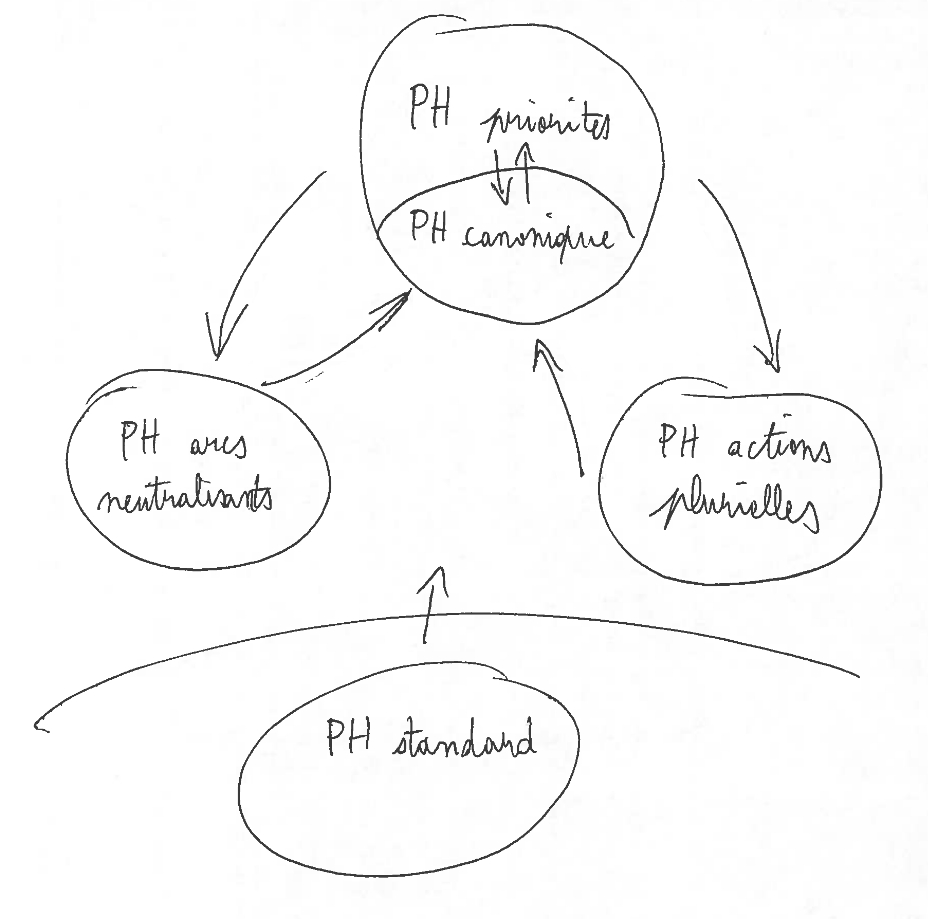
\includegraphics[height=.5\textheight]{figs/PH1.png}
% \end{center}

\setbeamercovered{transparent}

\begin{center}
\scalebox{.8}{
\begin{tikzpicture}
  \path[use as bounding box] (-5.2,-4) rectangle (5.2,3.5);
  \planPHstandard
  \planPHp
  \planPHan
  \planPHmult
  \planPHcanonique
  
  \uncover<2->{
    \path[draw, very thick, bend right=10] (-0.2,2.2) edge[->] (-.2,1.6);
    \path[draw, very thick, bend left=10] (0.2,2.2) edge[<-] (.2,1.6);
  }
  
  \uncover<3->{
    \path[draw, very thick, bend right=10] (-2,1.8) edge[->] (-3,.5);
    \path[draw, very thick, bend right=10] (-2,0) edge[->] (-1,1.1);
  }
  
  \uncover<4->{
    \path[draw, very thick, bend left=10] (2,1.8) edge[<-] (3,.5);
    \path[draw, very thick, bend left=10] (2,0) edge[<-] (1,1.1);
  }
  
  \uncover<5->{
    \planPHstandardligne
    \path[draw, very thick, bend left=10] (0,-1.9) edge[->] (0,-.8);
  }
\end{tikzpicture}
}
\end{center}

Toutes les sémantiques développées sont équivalentes
\begin{itemize}
  \item Importantes possibilités d'expression
  \item Au prix d'une complexité parfois exponentielle
  \item Toujours traduisibles en forme canonique
\end{itemize}

\end{frame}



\setbeamercovered{transparent}

\begin{frame}[c]
  \frametitle{Traductions depuis et vers d'autres modèles discrets}

% \begin{center}
% \hspace*{-1cm}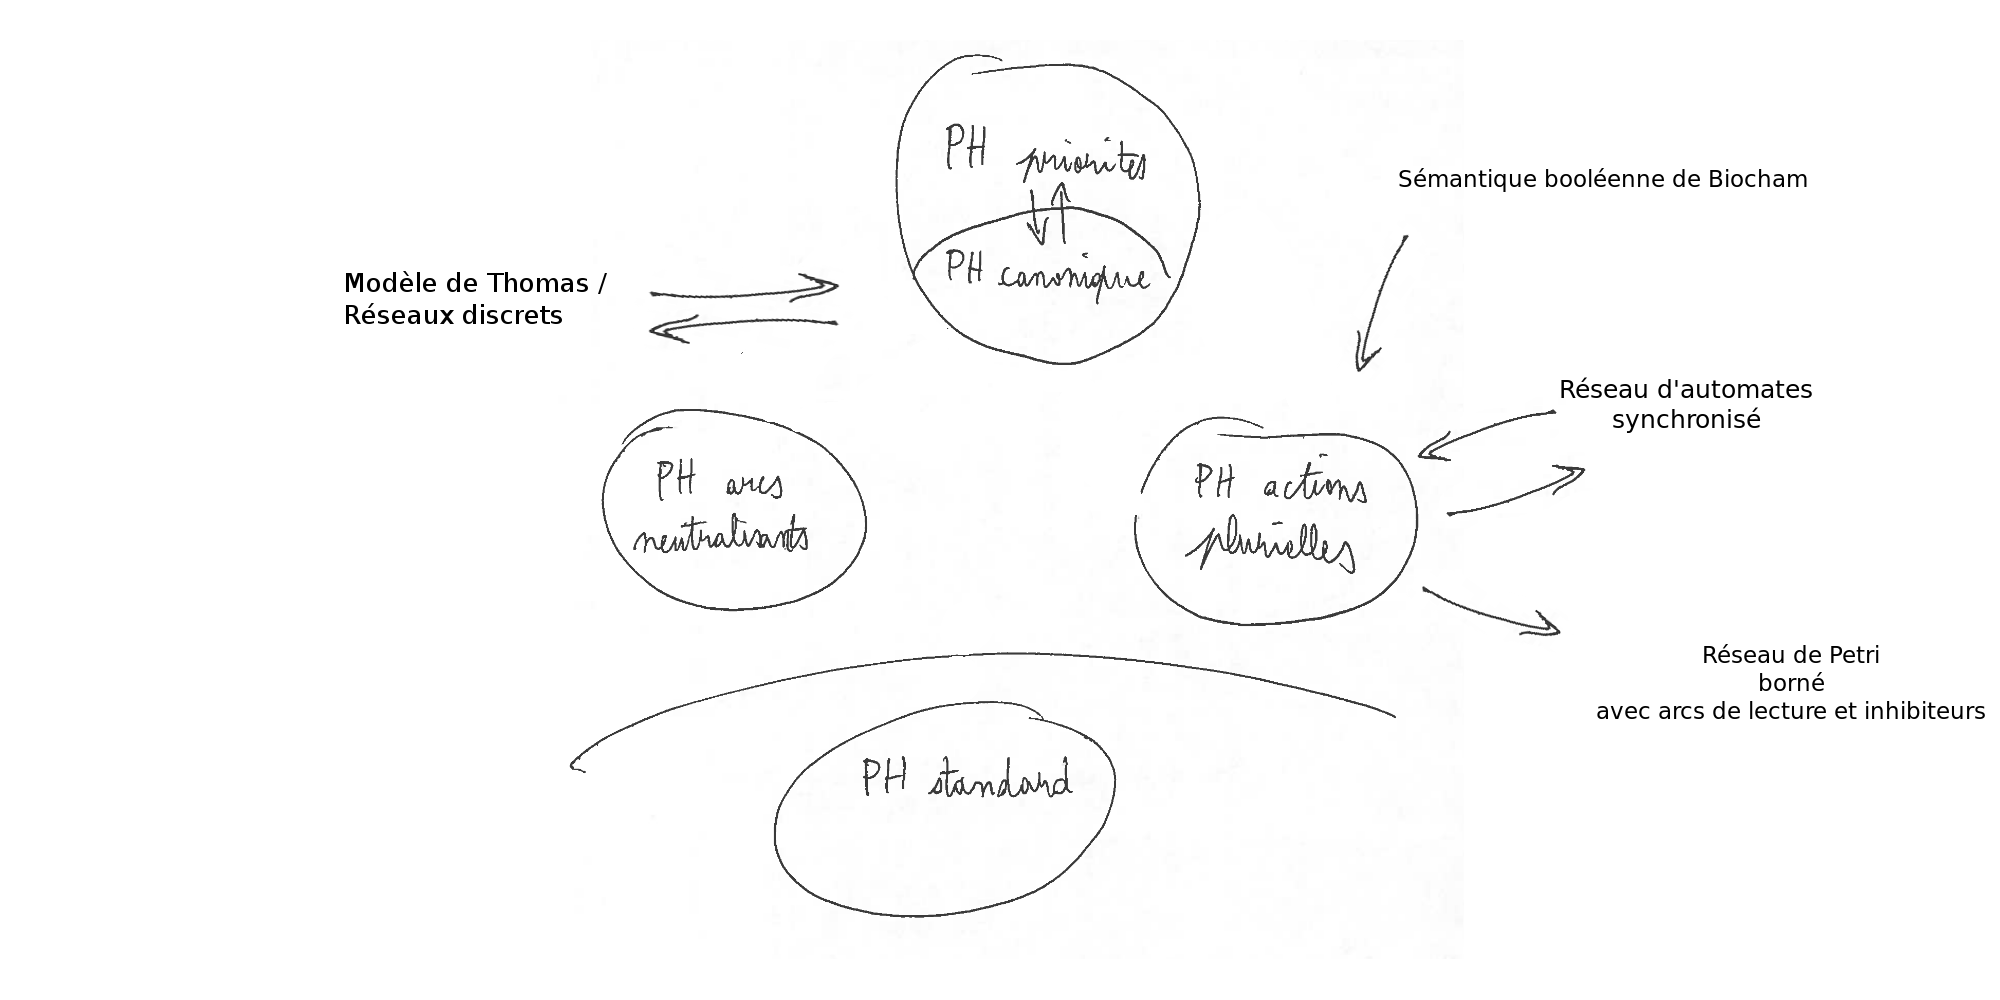
\includegraphics[height=.6\textheight]{figs/PH2.png}
% \end{center}

\begin{center}
\scalebox{.7}{
\begin{tikzpicture}
  \path[use as bounding box] (-5.2,-4) rectangle (5.2,3.5);
  \planPHstandard
  \planPHp
  \planPHan
  \planPHmult
  \planPHcanonique
  \planPHstandardligne
  
  \uncover<2->{
    \draw[thick, draw=black, fill=gray!10] (-4.5,2.5) ellipse (1.4 and .6)
      node[text width=4cm, align=center] {\small Modèle de Thomas\\Réseaux discrets};
    \path[draw, very thick, bend left=5] (-3.3,2.5) edge[->] (-1.5,1.4);
    \path[draw, very thick, bend right=5] (-3.4,2.3) edge[<-] (-1.6,1.2);
  }
  
  \uncover<3->{
    \draw[thick, draw=black, fill=gray!10] (6,2) ellipse (1.2 and .5)
      node[text width=4cm, align=center] {\small Automates\\synchronisés};
    \path[draw, very thick, bend left=5] (6,1.6) edge[->] (4.7,0.4);
    \path[draw, very thick, bend right=5] (5.7,1.7) edge[<-] (4.4,0.5);
  }
  
  \uncover<4->{
    \draw[thick, draw=black, fill=gray!10] (4.2,3.2) ellipse (1.7 and .5)
      node[text width=4cm, align=center] {\small Sémantique booléenne\\de Biocham};
    \path[draw, very thick, bend right=5] (4.2,2.8) edge[->] (3.7,0.6);
  }
  
  \uncover<5->{
    \draw[thick, draw=black, fill=gray!10] (6,-1.7) ellipse (1.7 and .5)
      node[text width=4cm, align=center] {\small Réseaux de Petri bornés\\avec arcs inhibiteurs};
    \path[draw, very thick, bend right=5] (5.7,-1.4) edge[<-] (4.2,-.6);
  }
\end{tikzpicture}
}
\end{center}

\begin{itemize}
  \item Équivalence avec les réseaux discrets / le modèle de Thomas
  \item Équivalence avec les réseaux d'automates synchronisés
  \item Traduction vers les réseaux de Petri (bornés) avec arcs inhibiteurs
  \item Traduction depuis la sémantique booléenne de Biocham.
\end{itemize}

\end{frame}

\setbeamercovered{invisible}

% Implémentation

\begin{frame}[c]
  \frametitle{Traduction en modèle de Thomas}
  \framesubtitle{\tcite{\cfpimrcmsb}}

\begin{itemize}
  \item Inférence du graphe des interactions, puis des paramètres
  \item Analyse exhaustive de la dynamique locale pour chaque régulateur
  \item Possibilité d'énumérer toutes les paramétrisations compatibles avec la dynamique
\end{itemize}

\bigskip
\tval{Complexité} :\\
\quad Linéaire dans le nombre de composants\\ %linear in the number of genes,\\
\quad Exponentielle dans le nombre de régulateurs de chaque composant %exponential in the number of regulators of one gene

\pause
\bigskip
\small
\begin{tabular}{r||c|c|c||c|c||c|c|}
\multicolumn{4}{c||}{Modèles} & \multicolumn{2}{c||}{Inférence du GI} & \multicolumn{2}{c|}{Inférence des paramètres}\\
\hline
\tval{Nom} & Sortes & Processus & Actions & $\Delta t$ & Arcs & $\Delta t$ & Paramètres\\
\hline
  \tval{\ex{egfr20}} & 22 & 152 & 399 & \tval{1s} & 50 & \tval{1s} & 191\\
\hline
  \tval{\ex{tcrsig40}} & 14 & 156 & 301 & \tval{1s} & 54 & \tval{1s} & 143\\
\hline
  \tval{\ex{tcrsig94}} & 39 & 448 & 1124 & \tval{13s} & 169 & $\infty$ & $2.10^9$\\
\hline
  \tval{\ex{egfr104}} & 89 & 748 & 2356 & \tval{4min} & 241 & \tval{1min 30s} & $1.10^6 / 2.10^6$\\
\hline
\end{tabular}

%S = Sortes \quad CS = Sortes coopératives \quad P = Processus \quad A = Actions

\footnotesize
\cmodels
\end{frame}


\section{Conclusion}
% Conclusion

\begin{frame}[c]
  \frametitle{Conclusion générale}

Les Frappes de Processus standard permettent une \tval{représentation atomique}\\
des réseaux de régulation biologique :
\begin{itemize}
  \item Analyse statique efficace existante
  \item Mais problèmes de décalage temporel
  \item Limites de modélisation
\end{itemize}

\medskip
\tval{Extensions des Frappes de Processus} pour augmenter l'expressivité :
\begin{itemize}
  \item Correction du décalage temporel \f expressivité strictement plus forte
  \item Possibilité de simuler des paramètres temporels
  \item Nouveaux liens avec d'autres formalismes (Thomas, RdP, etc.)
\end{itemize}

\medskip
Élargissement de l'\tval{analyse statique} à la forme canonique :
\begin{itemize}
  \item Analyse efficace de propriétés dynamiques
  \item Applicable aux différentes extensions au prix d'une traduction
  \item Nouveau type de propriétés : activation simultanée
\end{itemize}

% 
% 
% Process Hitting: an atomistic modeling with powerful static analysis
% 
% \medskip
% \begin{enumerate}[1.]
%   \item Stochastic parameters:
%     \begin{itemize}
%       \item To model systems with chronometric features
%       \item \tval{Continuous time}
%       \item But \tval{hard to analyze}
%     \end{itemize}
%   \item Classes of priorities:
%     \begin{itemize}
%       \item Allows to reproduce the same behaviors
%       \item Efficient \tval{static analysis}
%       \item But the translation to canonical form faces \tval{combinatorial explosion}
%     \end{itemize}
%   \item Neutralizing edges:
%     \begin{itemize}
%       \item Alternative to priorities
%       \item Closer to reality in some cases
%       \item \tval{Lighter translation} to canonical form
%     \end{itemize}
% \end{enumerate}
% 
% \vfill
% \Large
% \begin{flushright}
%   \tval{Thank you}\hspace{1cm}~
% \end{flushright}
% \vfill

\end{frame}

\setbeamercovered{invisible}



\begin{frame}[c]
  \frametitle{Ouvertures et perspectives}

Pistes d'\tval{exploitation} :
\begin{itemize}
  \item Modélisation et analyse de bases de données complètes
  \item Étude de comportements incontrôlables, de perturbations ponctuelles
  \item Recherche de propriétés intéressantes (attracteurs, oscillations...)
\end{itemize}

\medskip
Enrichissement de l'\tval{analyse statique} :
\begin{itemize}
  \item Raffinement pour réduire l'ensemble des cas non-conclusifs
  \item Utilisation de méthodes dérivées utilisant le graphe de causalité locale
  \item Développement de nouvelles propriétés (logiques temporelles, compteurs...)
\end{itemize}

\medskip
Enrichissement des \tval{capacités de représentation} :
\begin{itemize}
  \item Classes de priorités dynamiques
  \item Actions gardées ou portes logiques complexes
  \item Outils de vérification et correction (logique de Hoare)
\end{itemize}

\end{frame}



\begin{frame}[c]
  \frametitle{Collaborations}

Participation au projet \tval{ANR blanc BioTempo} (mars 2011 -- novembre 2014) :
\begin{center}
«~Représentations à l’aide de langage, de temps et de modèles hybrides\\
pour l’analyse de modèles incomplets en biologie moléculaire~»
\end{center}
Tâche 3 : Introduction de synchronisations\\
et de données chronométriques dans les modèles chronologiques

\bigskip
\bigskip
Stage doctoral de 3 mois (mars -- mai 2012) :\\
\tval{National Institute of Informatics} (Tokyo, Japon)\\
Invité dans l'équipe de \tval{Katsumi Inoue}
\begin{center}
«~Raisonnement automatisé et recherche d'hypothèses\\
pour la biologie des systèmes~»
\end{center}
Partenariat organisé par AtlanSTIC\\
participation financière de Centrale Initiatives



%\tval{Inoue Laboratory} (NII, Sokendai): Constraint Programming, Systems Biology

%\tval{MeForBio} (IRCCyN, ÉCN): Formal Methods for Bioinformatics

%\tval{AMIB} (LIX, Polytechnique): Algorithms and Models for Integrative Biology

% \bigskip\footnotesize
% \begin{center}
%   $\left.\text{\begin{tabular}{ccc}
%       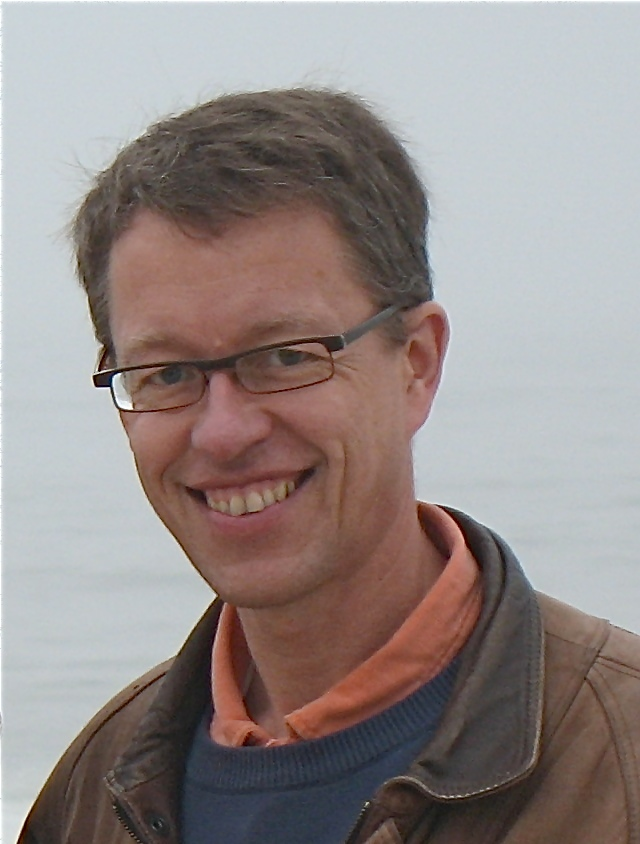
\includegraphics[height=1.5cm]{figs/Olivier.jpg}
%     & 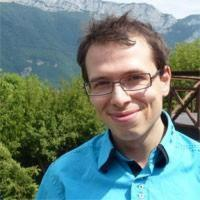
\includegraphics[height=1.5cm]{figs/Morgan.jpg} \\
%       \tval{Olivier ROUX} & \tval{Morgan MAGNIN} \\
%       Professeur \& chef d'équipe & Maître de conférences
%   \end{tabular}}\right\}$ %\text{\tval{MeForBio}}$%}
%   \parbox{2cm}{\tval{MeForBio}\\IRCCyN\\(Nantes, France)}
% 
%   \vspace*{3em}
%   $\left.\text{\begin{tabular}{c}
%     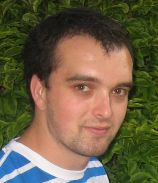
\includegraphics[height=1.5cm]{figs/Loic.jpg} \\ \tval{Loïc PAULEVÉ} \\ Chargé de recherche CNRS
%   \end{tabular}}\right\}$%\text{\tval{AMIB}}$
%   \parbox{1.5cm}{\tval{Bioinfo/AMIB}\\LRI\\(Orsay, France)}
%   \hspace*{3em}
%   $\left.\text{\begin{tabular}{c}
%     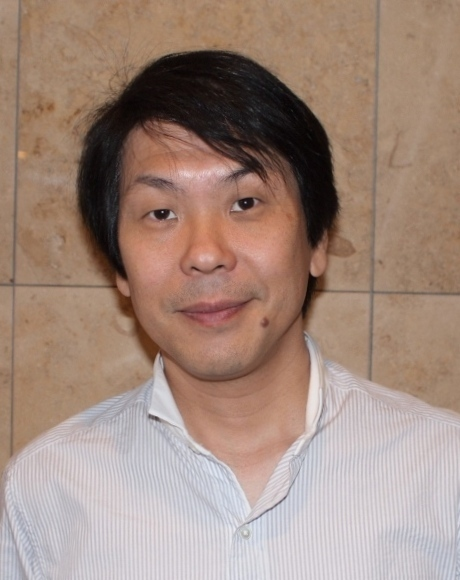
\includegraphics[height=1.5cm]{figs/Inoue-sensei.jpg} \\ \tval{Katsumi INOUE} \\ Professeur \& chef d'équipe
%   \end{tabular}}\right\}$%\text{\tval{Inoue Laboratory}}$
%   \parbox{1.5cm}{\tval{Inoue Lab.}\\NII\\(Tokyo, Japon)}
% \end{center}

\end{frame}



\begin{frame}[c]
  \frametitle{Contributions personnelles}

\small
\emphcolor{Chapitre de livre :}
\begin{itemize}
  \item Paulevé, Chancellor, \tval{Folschette}, Magnin, Roux :\\
    \tval{Analyzing Large Network Dynamics with Process Hitting},\\
    \textit{Logical Modeling of Biological Systems}, août 2014
\end{itemize}

\medskip
\emphcolor{Conférences et workshops :}
\begin{itemize}
  \item \tval{Folschette}, Paulevé, Magnin, Roux :\\
    \tval{Under-approximation of reachability in multivalued asynchronous networks},
    \begin{tikzpicture}
      \path[use as bounding box] (0,0) rectangle (0,.1);
      \path[grosarca, ->] (2,0.08) edge (.3,0.08);
      \path[grosarca, ->] (2,-3.45) edge (.3,-3.45);
      \path[grosarca] (2,0.08) edge (2,-3.45);
    \end{tikzpicture}\\
    CS2Bio'13, \textit{Electronic Notes in Theoretical Computer Science}, \vol 299, 2013\\
    \emphcolor{sélectionné pour un numéro spécial} de \textit{Theoretical Computer Science}
 \item \tval{Folschette}, Paulevé, Inoue, Magnin, Roux :\\
    \tval{Concretizing the process hitting into biological regulatory networks},
    \begin{tikzpicture}
      \path[use as bounding box] (0,0) rectangle (0,.1);
      \path[grosarcb, ->] (2,0.08) edge (0.3,0.08);
      \path[grosarcb, ->] (2,-0.9) edge (0.8,-0.9);
      \path[grosarcb, ->] (2,-3.15) edge (1.1,-3.15);
      \path[grosarcb] (2,0.08) edge (2,-3.15);
    \end{tikzpicture}\\
    CMSB'12, \textit{Lecture Notes in Computer Science}, 2012
  \item \tval{Folschette}, Paulevé, Inoue, Magnin, Roux :\\
    \tval{Abducing Biological Regulatory Networks from Process Hitting models},\\
    \textit{ECML-PKDD'12 / LDSSB'12}, 2012
\end{itemize}

\emphcolor{Soumissions de journaux en cours :}
\begin{itemize}
  \item \tval{Folschette}, Paulevé, Magnin, Roux :\\
    \tval{Sufficient Conditions for Reachability in Automata Networks with Priorities},\\
    \emphcolor{soumis} à un numéro spécial de \textit{Theoretical Computer Science}
  \item \tval{Folschette}, Paulevé, Inoue, Magnin, Roux :\\
    \tval{Constructing Biological Regulatory Networks from Process Hitting models},\\
    \emphcolor{en cours de révision} pour \textit{Theoretical Computer Science}
  \item Paulevé, \tval{Folschette}, Magnin, Roux :\\
    \tval{Analyses statiques de la dynamique des réseaux d'automates indéterministes},\\
    \emphcolor{soumis} à un numéro spécial de \textit{Technique et Science Informatiques}
\end{itemize}

\end{frame}



% 
% \begin{frame}[c]
%   \frametitle{Contributions personnelles}
% 
% \small
% \emphcolor{Chapitre de livre} avec Paulevé, Chancellor, Magnin, Roux :
% \begin{itemize}
%   \item \tval{Analyzing Large Network Dynamics with Process Hitting},\\
%     \textit{Logical Modeling of Biological Systems},
% %    éditeurs : Luis Farinas del Cerro et Katsumi Inoue,
%     2014%, ISBN 978-1-84821-680-8.
% \end{itemize}
% 
% \medskip
% \emphcolor{Workshop} avec Paulevé, Magnin, Roux :
% \begin{itemize}
%   \item \tval{Under-approximation of reachability in multivalued asynchronous networks},\\
%     CS2Bio'13,
%     %in: Proceedings of the fourth International Workshop on Interactions between Computer Science and Biology,
%     %éditeurs : Emanuela Merelli et Angelo Troina,
%     \textit{Electronic Notes in Theoretical Computer Science}, \vol 299, 2013\\
%     \emphcolor{sélectionné pour un numéro spécial} de \textit{Theoretical Computer Science}
%     %33--51, Springer Berlin Heidelberg, juin 2013, DOI 10.1016/j.entcs.2013.11.004.
%     %\emphcolor{Selected for a special issue in the journal \textit{Theoretical Computer Science}.}
% \end{itemize}
% 
% \emphcolor{Conférence et workshop} avec Paulevé, Inoue, Magnin, Roux :
% \begin{itemize}
%   \item \tval{Concretizing the process hitting into biological regulatory networks},\\ %\newline{}
%     CMSB'12, \textit{Lecture Notes in Computer Science}, %éditeurs : David Gilbert et Monika Heiner, %\newline{}
%     2012
%     %in: \textit{Computational Methods in Systems Biology}, éditeurs : David Gilbert et Monika Heiner, %\newline{}
%     %166--186, Springer Berlin Heidelberg, octobre 2012, DOI 10.1007/978-3-642-33636-2\_11.
%   \item \tval{Abducing Biological Regulatory Networks from Process Hitting models},\\
%     \textit{ECML-PKDD'12 / LDSSB'12}, %éditeurs : Oliver Ray et Katsumi Inoue,
%     2012
%     %24--35, septembre 2012.
% \end{itemize}
% 
% \emphcolor{Soumissions de journaux en cours :}
% \begin{itemize}
%   \item \tval{Folschette}, Paulevé, Magnin, Roux :\\
%     \tval{Sufficient Conditions for Reachability in Automata Networks with Priorities},\\
%     %version étendue de “Under-approximation of reachability in multivalued asynchronous networks”,
%     \emphcolor{soumis} à un numéro spécial de  de \textit{Theoretical Computer Science}% en avril 2014.
%   \item \tval{Folschette}, Paulevé, Inoue, Magnin, Roux :\\
%     \tval{Constructing Biological Regulatory Networks from Process Hitting models},\\
%     %extended version of “Concretizing the process hitting into biological regulatory networks”,
%     \emphcolor{en cours de révision} pour \textit{Theoretical Computer Science}
%   \item Paulevé, \tval{Folschette}, Magnin, Roux :\\
%     \tval{Analyses statiques de la dynamique des réseaux d'automates indéterministes},\\
%     \emphcolor{soumis} à un numéro spécial de \textit{Technique et Science Informatiques}
%     %editors: N.~Fatès and S.~Sené,
%     %\emphcolor{soumis} en avril 2014.
% \end{itemize}
% 
% \end{frame}

\section[x]{Merci pour votre attention}
% Merci !

\begin{frame}[c]

\vspace*{1cm}
\LARGE
\centering
\textbf{Merci pour votre attention}

\end{frame}


\appendix
\newcounter{finalframe}
\setcounter{finalframe}{\value{framenumber}}

\section[x]{Bibliographie}
% Bibliographie

\begin{frame}[c]
  \frametitle{Contributions personnelles}

\small
Chapitre de livre :
\begin{itemize}
  \item Loïc Paulevé, Courtney Chancellor, \emphcolor{Maxime Folschette}, Morgan Magnin et Olivier Roux :
    \emphcolor{Analyzing Large Network Dynamics with Process Hitting},
    \textit{Logical Modeling of Biological Systems},
    éditeurs : Luis Farinas del Cerro et Katsumi Inoue,
    août 2014, ISBN 978-1-84821-680-8.
\end{itemize}

\medskip
Conférences et workshops :
\begin{itemize}
  \item \emphcolor{Maxime Folschette}, Loïc Paulevé, Morgan Magnin et Olivier Roux :
    \emphcolor{Under-approximation of reachability in multivalued asynchronous networks},
    in: Proceedings of the fourth International Workshop on Interactions between Computer Science and Biology, éditeurs : Emanuela Merelli et Angelo Troina,
    \textit{Electronic Notes in Theoretical Computer Science}, \vol 299,
    33--51, Springer Berlin Heidelberg, juin 2013, DOI 10.1016/j.entcs.2013.11.004.
    %\emphcolor{Selected for a special issue in the journal \textit{Theoretical Computer Science}.}
  \item \emphcolor{Maxime Folschette}, Loïc Paulevé, Katsumi Inoue, Morgan Magnin et Olivier Roux :
    \emphcolor{Concretizing the process hitting into biological regulatory networks}, %\newline{}
    in: \textit{Computational Methods in Systems Biology}, éditeurs : David Gilbert et Monika Heiner, %\newline{}
    166--186, Springer Berlin Heidelberg, octobre 2012, DOI 10.1007/978-3-642-33636-2\_11.
  \item \emphcolor{Maxime Folschette}, Loïc Paulevé, Katsumi Inoue, Morgan Magnin et Olivier Roux :
    \emphcolor{Abducing Biological Regulatory Networks from Process Hitting models},
    in: \textit{ECML-PKDD 2012 Workshop on Learning and Discovery in Symbolic Systems Biology}, éditeurs : Oliver Ray et Katsumi Inoue,
    24--35, septembre 2012.
\end{itemize}

\end{frame}



\begin{frame}[c]
  \frametitle{Bibliography}

%\footnotesize
\small
\setlength{\parindent}{-1em}
\setlength{\parskip}{0.5em}

\tcitebullet Loïc Paulevé, Morgan Magnin, Olivier Roux. \ex{Refining dynamics of gene regulatory networks in a stochastic $\pi$-calculus framework}. In Corrado Priami, Ralph-Johan Back, Ion Petre, and Erik de Vink, editors: \textit{Transactions on Computational Systems Biology XIII}, volume 6575 of Lecture Notes in Computer Science, pages 171--191, 2011.

\tcitebullet Loïc Paulevé, Morgan Magnin, Olivier Roux. \ex{Static analysis of biological regulatory networks dynamics using abstract interpretation}. \textit{Mathematical Structures in Computer Science}, 2012.

%\tcitebullet Adrien Richard, Jean-Paul Comet, Gilles Bernot. \ex{R. Thomas' logical method}, 2008. Invited at \textit{Tutorials on modelling methods and tools: Modelling a genetic switch and Metabolic Networks}, Spring School on Modelling Complex Biological Systems in the Context of Genomics.

%\tcitebullet Adrien Richard, Jean-Paul Comet, Gilles Bernot. \textit{Modern Formal Methods and App.}, chapter \ex{Formal Methods for Modeling Biological Regulatory Networks}, pages 83--122, 2006.

%\tcitebullet Maxime Folschette, Loïc Paulevé, Katsumi Inoue, Morgan Magnin, Olivier Roux. \ex{Concretizing the Process Hitting into Biological Regulatory Networks}. In David Gilbert and Monika Heiner, editors, \textit{Computational Methods in Systems Biology X}, Lecture Notes in Computer Science, pages 166--186. Springer Berlin Heidelberg, 2012.

\tcitebullet Maxime Folschette, Loïc Paulevé, Morgan Magnin, Olivier Roux. \ex{Under-approximation of Reachability in Multivalued Asynchronous Networks}. In E. Merelli and A. Troina, editors, \textit{4th International Workshop on Interactions between Computer Science and Biology (CS2Bio’13)}, Electronic Notes in Theoretical Computer Science, Volume 299, 33–51. June 2013.

\tcitebullet Loïc Paulevé. PhD thesis: \ex{\textit{Modélisation, Simulation et Vérification des Grands Réseaux de Régulation Biologique}}, October 2011, Nantes, France.

%\tcitebullet Loïc Paulevé, Morgan Magnin, and Olivier Roux. \textit{Tuning Temporal Features within the Stochastic $\pi$-Calculus}. IEEE Transactions on Software Engineering, 37(6), pages 858--871, 2011.

%\tcitebullet Loïc Paulevé and Adrien Richard. \textit{Topological Fixed Points in Boolean Networks}. Comptes Rendus de l'Académie des Sciences - Series I - Mathematics, 348(15-16), pages 825--828, 2010.

%\tcitebullet Gilles Bernot, Franck Cassez, Jean-Paul Comet, Franck Delaplace, Céline Müller, Olivier Roux. \ex{Semantics of Biological Regulatory Networks}. \textit{Proceedings of the First Workshop on Concurrent Models in Molecular Biology}, Electronic Notes in Theoretical Computer Science 180(3), pages 3--14, 2007.

%\tcitebullet Adrien Richard. \ex{Negative circuits and sustained oscillations in asynchronous automata networks}. \textit{Advances in Applied Mathematics} 44(4), pages 378--392, 2010.

\tcitebullet Paul François, Vincent Hakim, Eric D Siggia. \ex{Deriving structure from evolution : metazoan segmentation}.
In \textit{Molecular Systems Biology}, Volume 3, Issue 1. 2007.

\end{frame}


\section{Analyse statique des Frappes de Processus standards}
% Exemples de structures abstraites (graphes de causalité locale)

\begin{frame}
  \frametitle{Static analysis: successive reachability}
  \framesubtitle{\tcite{\cpmrmscs}}

Successive reachability of processes:

\begin{columns}
\begin{column}{0.55\textwidth}

\begin{center}
\scalebox{0.75}{
\begin{tikzpicture}
  %\path[use as bounding box] (-1,-3) rectangle (7,2);
  \exatt

  \TState{1-5}{a_0,b_0,c_0,d_0}
  \TState{6}{a_0,b_0,c_1,d_0}
  \TState{7}{a_0,b_0,c_1,d_1}
  \TState{8}{a_0,b_1,c_1,d_1}
  \node<9>[process,very thick] (d_2) at (d_2.center) {};
  \TState{9}{a_0,b_1,c_1,d_2}

  \node<2>[objective] at (d_1.center) {1?};
  \node<2>[objective] at (d_2.center) {2?};

  \node<3>[objective] at (d_1.center) {1?};
  \node<3>[objective] at (b_1.center) {2?};
  \node<3>[objective] at (d_2.center) {3?};

  \node<4-8>[objective] at (d_2.center) {1?};

  %\node<3>[process,very thick] (d_1) at (d_1.center) {1?};
  %\node<3>[process,very thick] (b_1) at (b_1.center) {2?};
  %\node<3>[process,very thick] (d_2) at (d_2.center) {3?};

  %\node<4-8>[process,very thick] (d_2) at (d_2.center) {1?};

  \only<5>{\THit{a_0}{hlhit}{c_0}{.north}{c_1}}
  \path<5>[bounce,bend left,hlhit] \TBounce{c_0}{}{c_1}{.west};
  \only<6>{\THit{b_0}{hlhit}{d_0}{.west}{d_1}}
  \path<6>[bounce,bend left,hlhit] \TBounce{d_0}{}{d_1}{.south};
  \only<7>{\THit{c_1}{bend left=20pt,hlhit}{b_0}{.west}{b_1}}
  \path<7>[bounce,bend left,hlhit] \TBounce{b_0}{}{b_1}{.south};
  \only<8>{\THit{b_1}{hlhit}{d_1}{.west}{d_2}}
  \path<8>[bounce,bend left,hlhit] \TBounce{d_1}{}{d_2}{.south};
\end{tikzpicture}
}
\end{center}

\end{column}
\begin{column}{0.45\textwidth}

%\pause
~\\~\\
\begin{itemize}
  \item Initial state
    \\ \rex{\PHetat{a_1, b_0, c_0, d_0}} \pause
  \item Objectives
    \\ \rex{$[\ \Rsh d_1\ \PHconcat\ \Rsh d_2\ ]$} \pause
    \\\smallskip \rex{$[\ \Rsh d_1 \PHconcat\ \Rsh b_1 \PHconcat\ \Rsh d_2\ ]$} \pause
    \\\smallskip \rex{$[\ \Rsh d_2\ ]$} \pause
\end{itemize}

\end{column}
\end{columns}

\medskip
\begin{center}
\f Concretization of the objective = scenario

\ex{
$ \only<5>{\underline{\PHfrappe{a_0}{c_0}{c_1}}} \only<-4,6->{\PHfrappe{a_0}{c_0}{c_1}} \PHconcat %
  \only<6>{\underline{\PHfrappe{b_0}{d_0}{d_1}}}\only<-5,7->{\PHfrappe{b_0}{d_0}{d_1}} \PHconcat %
  \only<7>{\underline{\PHfrappe{c_1}{b_0}{b_1}}}\only<-6,8->{\PHfrappe{c_1}{b_0}{b_1}} \PHconcat %
  \only<8>{\underline{\PHfrappe{b_1}{d_1}{d_2}}}\only<-7,9->{\PHfrappe{b_1}{d_1}{d_2}}
$}
\end{center}
\end{frame}



\begin{frame}
  \frametitle{Over- and Under-approximations}
  \framesubtitle{\tcite{\cpmrmscs}}

Static analysis by abstractions:
\begin{fleches}
  \item Directly checking an objective sequence $R$ is hard
  \item Rather check the approximations $P$ and $Q$, where \tval{$P \Rightarrow R \Rightarrow Q$}:
\end{fleches}

\begin{center}
\scalebox{0.6}{
\figsa
}
\end{center}

\only<-7>{~}
\only<8->{
Polynomial w.r.t.~the number of sorts and \\exponential w.r.t.~the number of processes in each sort
\begin{fleches}
  \item Efficient for big models with few levels of expression
\end{fleches}
}
\end{frame}



\begin{frame}
  \frametitle{Under-approximation}

\def \tu {2}
\def \tub {3}
\def \tuf {4}

\begin{columns}
\begin{column}{0.48\textwidth}

\begin{center}
\scalebox{0.55}{
\begin{tikzpicture}
  \exatt
  \TState{-\tu}{a_1,b_1,c_1,d_0}
  \TState{\tub-}{a_0,b_1,c_0,d_0}
  \node[objective] (d_2) at (d_2.center) {?};
\end{tikzpicture}
}
\end{center}

\end{column}
\begin{column}{0.52\textwidth}

\vspace{1.5em}
\tval{Sufficient condition}:

\smallskip
\begin{itemize}
  \item no cycle
  \item \only<-\tu>{each objective has a solution} \only<\tub->{\sout{each objective has a solution}}
\end{itemize}
\begin{center}
  \only<\tu>{\Large\textcolor{darkgreen}{$R$ is \textbf{true}}} \only<\tuf>{\Large\textcolor{darkyellow}{\textbf{Inconclusive}}}
\end{center}

\end{column}
\end{columns}

\begin{center}%
%\vspace*{1cm}%
\scalebox{\scaleex}{%
\only<-\tu>{%
\scalebox{\scaleex}{%
\begin{tikzpicture}[aS]
  \path[use as bounding box] (.7,1) rectangle (5.8,2.5);

  \glclegend{}{$d_2$}{$\PHobj{d_0}{d_2}$}
\end{tikzpicture}
}
  \sauyes
}
\only<\tub->{
  \sauinconc
}}
\end{center}
\end{frame}



\begin{frame}
  \frametitle{Over-approximation}

\def \to {4}
\def \tob {5}
\def \tof {6}
\def \tokp {7}

\begin{columns}
\begin{column}{0.48\textwidth}

\begin{center}
\scalebox{0.55}{
\begin{tikzpicture}
  \exatt
  \TState{-\to}{a_1,b_0,c_0,d_1}
  \TState{\tob-}{a_1,b_1,c_1,d_0}
  \node[objective] (d_2) at (d_2.center) {?};
\end{tikzpicture}
}
\end{center}
\bigskip

\end{column}
\begin{column}{0.52\textwidth}

\tval{Necessary condition}:

\smallskip
\only<2->{
\only<3-\to>{\sout{There exists a traversal}}\only<2,\tob->{There exists a traversal}
with no cycle

\smallskip
\begin{itemize}
  \item \only<3-\to>{\sout{objective $\rightarrow$ follow one solution}}\only<1-2,\tob->{objective $\rightarrow$ follow one solution}
  \item solution $\rightarrow$ follow all processes
  \item process $\rightarrow$ follow all objectives
\end{itemize}
\begin{center}
  \only<\to>{\Large\textcolor{red}{$R$ is \textbf{false}}}\only<\tof->{\Large\textcolor{darkyellow}{\textbf{Inconclusive}}}
\end{center}
}

\end{column}
\end{columns}

\begin{center}
\scalebox{\scaleex}{
\only<1-\to>{
  \saono
}
\only<\tob->{
  \saoinconc
}}
\end{center}
\end{frame}


% 
% \begin{frame}[c]
%   \frametitle{Implementation \& Execution times}
% 
% \Pint\tval{: Existing free OCaml library}
% 
% \medskip
% \f Compiler + tools for Process Hitting models
% 
% \f Documentation \& examples: \lien{http://processhitting.wordpress.com/}
% 
% \pause
% \bigskip
% \medskip
% \tval{Computation time for various reachability analyses:}
% 
% \medskip
% \small
% \begin{tabular}{r||c|c|c|c||c|c|c|}
% \hline
% \tval{Model} & Sorts & Procs & Actions & States & Biocham$^1$ & libddd$^2$ & \Pint \\\hline
% \tval{\ex{egfr20}} & 35 & 196 & 670 & $2^{64}$ & [3s--$\infty$] & [1s--150s] & \tval{0.007s} \\\hline
% \tval{\ex{tcrsig40}} & 54 & 156 & 301 & $2^{73}$ & [1s--$\infty$] & [0.6s--$\infty$] & \tval{0.004s} \\\hline
% \tval{\ex{tcrsig94}} & 133 & 448 & 1124 & $2^{194}$ & $\infty$ & $\infty$ & \tval{0.030s} \\\hline
% \tval{\ex{egfr104}} & 193 & 748 &  2356 & $2^{320}$ &  $\infty$ & $\infty$ & \tval{0.050s}\\\hline
% \end{tabular}
% 
% \medskip
% \quad$^1$ Inria Paris-Rocquencourt/Contraintes\\
% \quad$^2$ LIP6/Move
% 
% \cmodels
% \end{frame}

% Recherche de points fixes par n-cliques

\begin{frame}[c]
  \frametitle{Static Analysis: Fixed Points}
  \framesubtitle{\tcite{\cpmrtcsb}}

\tval{Fixed point} = state where no action can be fired
\begin{fleches}
  \item avoid couples of processes bounded by an action
\only<1>{\\\smallskip~}
\only<2->{\item Hitless Graph \only<3->{\f \tval{n-cliques} = fixed points}}
\end{fleches}

\bigskip
\begin{columns}
\begin{column}{0.5\textwidth}

\begin{center}
\scalebox{0.7}{
\begin{tikzpicture}
\exdefb
\exdefbfrappes
\end{tikzpicture}
}
\end{center}

\end{column}
\begin{column}{0.5\textwidth}

\only<2->{
\begin{center}
\scalebox{0.7}{
\tikzstyle{current process}=[process,fill=red]
\begin{tikzpicture}[hitless graph]
\exdefb
\exdefbsf
\end{tikzpicture}
\tikzstyle{current process}=[process,fill=blue]
}
\end{center}
}

\end{column}
\end{columns}

\bigskip
\pause[6]
Exponential complexity w.r.t.~the number of sorts

\end{frame}


\setcounter{framenumber}{\value{finalframe}}

\end{document}
